%=========================================================================================================

\documentclass[12pt,a4paper]{article}

%% arquivo de definições de estilo documento
%==========================================================================================
% Pacotes

%% definições relacionadas a idioma
\usepackage[brazil]{babel}

%% codificação de caracteres
%% http://tex.stackexchange.com/questions/664/why-should-i-use-usepackaget1fontenc
%% http://tex.stackexchange.com/questions/44694/fontenc-vs-inputenc
\usepackage[T1]{fontenc}
\usepackage[utf8]{inputenc}    % usar se salvar com codificação UTF-8
%\usepackage[latin1]{inputenc}  % usar se salvar com codificação ISO

%% definições das margens
\usepackage[top=3cm,left=3cm,right=2cm,bottom=2cm]{geometry}

%% para inserir figuras em diversas extensões
\usepackage{graphicx}

%% controla o uso de Teorema, Definição, Exemplo, Demonstração, Exercício
\usepackage{amsthm}

%% todos os pacotes da AMS (American Mathematical Society), inúmeros símbolos
\usepackage{amsfonts,amssymb,amsxtra,empheq}  
\usepackage[mathscr]{eucal}

%% permite o uso de vírgula como separador decimal no ambiente matemático
\usepackage{icomma} 

%% permite o uso de comentários entre \begin{comment}...\end{comment}                 
\usepackage{comment}

%% cores em palavras, frases, etc. \textcolor{red}{text in red}
\usepackage{color}

%% permite a indentação do 1º paragráfo após um título de seção, capítulo
\usepackage{indentfirst}
%%%% recuo da primeira linha de cada parágrafo
\setlength{\parindent}{1.25cm}

%% permite a construção do texto colunas
\usepackage{multicol}

%% controla o espaçamento entre linhas
%\usepackage{setspace}
%%%% espaçamento 1.5 linha no texto \begin{spacing}{1.0}...\end{spacing}
%\onehalfspace   

%% permite desenhar
%% http://www.texample.net/tikz/
%\usepackage{tikz}
%\usetikzlibrary{decorations.pathreplacing}
%\usetikzlibrary{arrows,decorations.pathmorphing}
%\usetikzlibrary{shapes,backgrounds}  
  
%% para colocar a legenda indentada como formato da UFLA
\usepackage[format=hang, labelsep=endash]{caption}
%\usepackage[format=hang, labelsep=endash, singlelinecheck=false, margin={2cm,1cm}]{caption}
%% controla objetos flutuantes e permite definir novas classes
%% útil para criar a classe de fluantes 'program', para código
\usepackage{float}
%%%% algumas formas de denifir
%   \floatstyle{ruled}
%   \newfloat{Input}{tbp}{lop}[section]
%   \floatname{Input}{Program}

%% controla novos ambientes que listam índices, e.g. lista de anexos
\usepackage{listings}

%% texto em caixas
\usepackage{boxedminipage}

%% controle e definição de ambientes numerados
%% listas mais compactas, úteis para salvar espaço
%% http://tex.stackexchange.com/questions/62009/paralist-environment
\usepackage{paralist}

%% para rotacionar tabela \begin{sidewaystable}
\usepackage{rotating} 

%% rotacionar texto \begin{landscape}
\usepackage{lscape} 

%% para ter tabelas com linhas mescladas
\usepackage{multirow}

%% para inserir epigrafe
\usepackage{epigraph}

%% tabelas 
\usepackage{tabularx}

%% notas de rodapé
%\usepackage[symbol, hang, flushmargin]{footmisc} 

% controle e definições para tamanho de colunas em tabelas
\usepackage{array} 
%\newcolumntype{C}[1]{>{\centering\let\newline\\\arraybackslash\hspace{0pt}}m{#1}}
%\newcolumntype{R}[1]{>{\raggedleft\let\newline\\\arraybackslash\hspace{0pt}}m{#1}}
%\newcolumntype{R}{>{\raggedleft\let\newline\\\arraybackslash\hspace{0pt}}X}

\newcolumntype{L}[1]{>{\raggedright\let\newline\\\arraybackslash\hspace{0pt}}m{#1}}
\newcolumntype{C}[1]{>{\centering\let\newline\\\arraybackslash\hspace{0pt}}m{#1}}
%\newcolumntype{R}[1]{>{\raggedleft\let\newline\\\arraybackslash\hspace{0pt}}m{#1}}
\newcolumntype{R}{>{\raggedleft\let\newline\\\arraybackslash\hspace{0pt}}X}


\usepackage{tocbasic}
\usepackage{pdfpages}

% para a lista de figuras 
\DeclareTOCStyleEntry[
  entrynumberformat=\entrynumberwithprefix{\figurename},
  dynnumwidth,
  numsep=1em
]{tocline}{figure}
\newcommand\entrynumberwithprefix[2]{#1\enspace#2  -\hfill}

% para lista de tabelas
\DeclareTOCStyleEntry[
  entrynumberformat=\entrynumberwithprefix{\tablename},
  dynnumwidth,
  numsep=1em
]{tocline}{table}
\newcommand\entrynumberwithprefixd[2]{#1\enspace#2  -\hfill}

%==========================================================================================
% Definições

%% redefine o espaçamento entre linhas
\renewcommand{\baselinestretch}{1.2cm}
\def\onehalspacing{1.5}


%% permite leitura do caracter @ nas definições que seguem
\makeatletter

%%.....................................................
%% Sessões

%% definição do texto título da sessão
\renewcommand{\section}{\@startsection
{section}%                     % the name
{1}%                           % the level
{0mm}%                         % the indent
{-\baselineskip}%              % the before skip
{1.\baselineskip}%             % the after skip
{\noindent\normalsize\textbf}} % the style

%% definição do texto título da subsessão
\renewcommand{\subsection}{\@startsection
{subsection}%                  % the name
{2}%                           % the level
{0mm}%                         % the indent
{-\baselineskip}%              % the before skip
{0.001\baselineskip}%            % the after skip
{\noindent\normalsize}} % the style

%% definição do texto título da subsubsessão
\renewcommand{\subsubsection}{\@startsection
{subsubsection}%                  % the name
{2}%                           % the level
{0mm}%                         % the indent
{-\baselineskip}%              % the before skip
{0.001\baselineskip}%            % the after skip
{\noindent\normalsize\textbf}} % the style


%\makeatother


%% desabilita o uso do @
\makeatother

%%.....................................................
%% Sumário

%% sumário alinhado à esquerda
\usepackage{titletoc}
\def\distnumber{3.3em}

\titlecontents{section}       % set formatting for \section
[\distnumber]                 % adjust left margin
{\bfseries}                   % font formatting
{\contentslabel{\distnumber}} % section label and offset
{\hspace*{-\distnumber}}
{\normalfont\titlerule*[1pc]{.}\contentspage}

\titlecontents{subsection}    % set formatting for \subsection
[\distnumber]                 % adjust left margin
{\normalfont}                   % font formatting
{\contentslabel{\distnumber}} % section label and offset
{\hspace*{-\distnumber}}
{\normalfont\titlerule*[1pc]{.}\contentspage}

\titlecontents{subsubsection} % set formatting for \subsubsection
[\distnumber]                 % adjust left margin
{\bfseries}                   % font formatting
{\contentslabel{\distnumber}} % section label and offset
{\hspace*{-\distnumber}}
{\normalfont\titlerule*[1pc]{.}\contentspage}

\setcounter{tocdepth}{4}
\renewcommand{\baselinestretch}{1.5} % espaçamento entre linha
\numberwithin{equation}{section}     % numerar equação por seção

%%.....................................................
%% Flutuantes e equações

%% nomes
\renewcommand{\figurename}{Figura}
\renewcommand{\tablename}{Tabela}

%% profundidade de numeração
%\numberwithin{figure}{section}
%\numberwithin{table}{section}
%\numberwithin{equation}{section}

%%.....................................................
%% Paginação

\usepackage{fancyhdr}
\renewcommand{\headrulewidth}{0pt}
\fancyhf{}
\fancyhead[R]{\thepage}
\setlength{\headheight}{10pt}

%%.....................................................
%% Fontes

%% fonte para o texto
\usepackage{times}

%% fonte para ambiente matemático mais parecido com Times
\usepackage{txfonts}

%% fonte para ambiente de código (monospaced)
\usepackage[scaled=0.85]{beramono}

%%.....................................................
%% Referências e hyperlinks

\usepackage{hyperref} %transformas o sumário e as citações em hiperlinks
\hypersetup{
%    bookmarks=true,         % show bookmarks bar?
%    unicode=false,          % non-Latin characters in Acrobat's bookmarks
%    pdftoolbar=true,        % show Acrobat's toolbar?
%    pdfmenubar=true,        % show Acrobat's menu?
%    pdffitwindow=true,      % page fit to window when opened
  pdftitle={O seguro rural no Brasil},
  pdfauthor={Walef Machado de Mendonça},
  pdfsubject={Dissertação de Mestrado},
  pdfcreator={Walef Machado de Mendonça},
  pdfproducer={Walef Machado de Mendonça},
  %pdfkeywords={Verossimilhança, Curvatura, Método delta, van Genuchten},
%    pdfnewwindow=true,      % links in new window
  colorlinks=true,           % false: boxed links; true: colored links
  linkcolor=black,           % color of internal links
  citecolor=black,           % color of links to bibliography
  filecolor=red,             % color of file links
  bookmarksopen=false,
  urlcolor=cyan              % color of external linkss
}

% Para multiplas figuras
\usepackage[position=bottom]{subfig}
%\usepackage[labelsep=endash]{caption}
%\captionsetup[figure]{font=small,singlelinecheck=off}
%\captionsetup[figure]{format=hang,labelsep=endash,font=small,singlelinecheck=off, margin=1cm}
\captionsetup[subfigure]{textfont=small,singlelinecheck=off,justification=raggedright}

\usepackage[alf,bibjustif]{abntex2cite}
\usepackage{enumitem} % Para o enumerate
%%.....................................................
%% Comandos

\newcommand{\lin}{\noindent \rule[4mm]{\textwidth}{0.1ex}}

\renewcommand\UrlFont{\color{black}\rmfamily} 
\usepackage{url}
\DeclareUrlCommand\url{\def\UrlLeft{}\def\UrlRight{}}

%%  Inserindo os códigos Python ==================================
\usepackage{listings}

\definecolor{light_gray}{rgb}{0.97,0.97,0.97}
\definecolor{mymauve}{rgb}{0.58,0,0.82}
\definecolor{mygreen}{rgb}{0,0.6,0}
\lstset{
  basicstyle=\ttfamily,
  inputencoding = utf8,
  language = Python,
  backgroundcolor = \color{white},
  columns=fullflexible,
  breaklines=true,
  postbreak=\raisebox{0ex}[0ex][0ex]{\color{red}$\hookrightarrow$\space},
  keywordstyle=\color{black},      % keyword style
  stringstyle=\color{black},
  commentstyle=\color{black}
}



%==========================================================================================


%% para referencias bibliográficas no padrão ABNT
%\usepackage[abnt-substyle=UFLA,abnt-emphasize=bf,abnt-etal-list=3,abnt-and-type=e]{abntcite}

%=========================================================================================================
% Definições de conteúdo

%% título em português e inglês e caixa alta
\def\tesetitle{A distribuição espacial do seguro rural no Brasil}
%\def\tesetitleeng{Interpretable parametrization in nonlinear models}
\def\tesetitlecap{\expandafter\MakeUppercase\expandafter{\tesetitle}}

%% autor e abreviações
\def\teseauthor{Walef Machado de Mendonça}
\def\teseauthorcap{\expandafter\MakeUppercase\expandafter{\teseauthor}}
\def\teseauthorrev{Mendonça, Walef Machado}
\def\teseauthorcrv{MENDONCA, Walef Machado}

%% ano
\def\teseyear{2022}

%% orientador
\def\teseorientador{Patrícia de Siqueira Ramos}

%% palavras com infenização manual (não contidas no dicionário)
\hyphenation{ne-ces-s\'arias fa-zen-do pa-r\^{a}-me-tro a-va-li-ar vi-san-do pr\'o-prias
              Ge-nu-chten fi-ca-ram a-do-\c{c}\~ao in-ter-pre-t\'a-veis mo-no-mo-le-cu-lar
              re-pa-ra-me-tri-z\'a-lo}

\begin{document}
\pagestyle{empty}

%=========================================================================================================

%% inclui as capas, folhas de rosto, etc
%=========================================================================================================
% capa

\setcounter{page}{0}

	
%CAPA
\onehalfspacing
\thispagestyle{empty}
\begin{center}
	{\textbf{UNIVERSIDADE FEDERAL DE ALFENAS}}\\
	\vspace{6cm}
    {\textbf{\teseauthorcap}}\\
	\vspace{6cm}
    {\textbf{\tesetitlecap}} 
	%\vspace{7cm}\\
	\vfill
	\textbf{ALFENAS     / MG\\
		2022}
\end{center}

% página em branco
%\newpage\null\thispagestyle{empty}\newpage

%=========================================================================================================
% folha de rosto

\newpage
%\section*{}
\vspace{-0.7cm}
\centerline{\textbf{\teseauthorcap}}
\vspace{3cm}
\begin{singlespace}
\begin{center}
\textbf{\tesetitlecap}
\end{center}
\end{singlespace}
\vspace{3cm}
\begin{flushright}
\begin{minipage}{12cm}
\begin{quote}
\begin{singlespace}
Dissertação apresentada à Universidade Federal de Alfenas, como parte dos requisitos para obtenção do título de Mestre em Estatística Aplicada e Biometria. Área de concentração: Estatística Aplicada e Biometria. Linha de pesquisa: Modelagem Estatística e Estatística Computacional. 

\vspace{0.1cm}
\noindent Orientadora: Prof. Dra. \teseorientador
\end{singlespace}
\end{quote}
\end{minipage}
\end{flushright}


\begin{center}
\begin{singlespace}
%\noindent Orientador\\
%\noindent Prof. Dr. \teseorientador

\vfill

\textbf{ALFENAS / MG\\ \teseyear}
\end{singlespace}
\end{center}

%=========================================================================================================
% ficha catalográfica
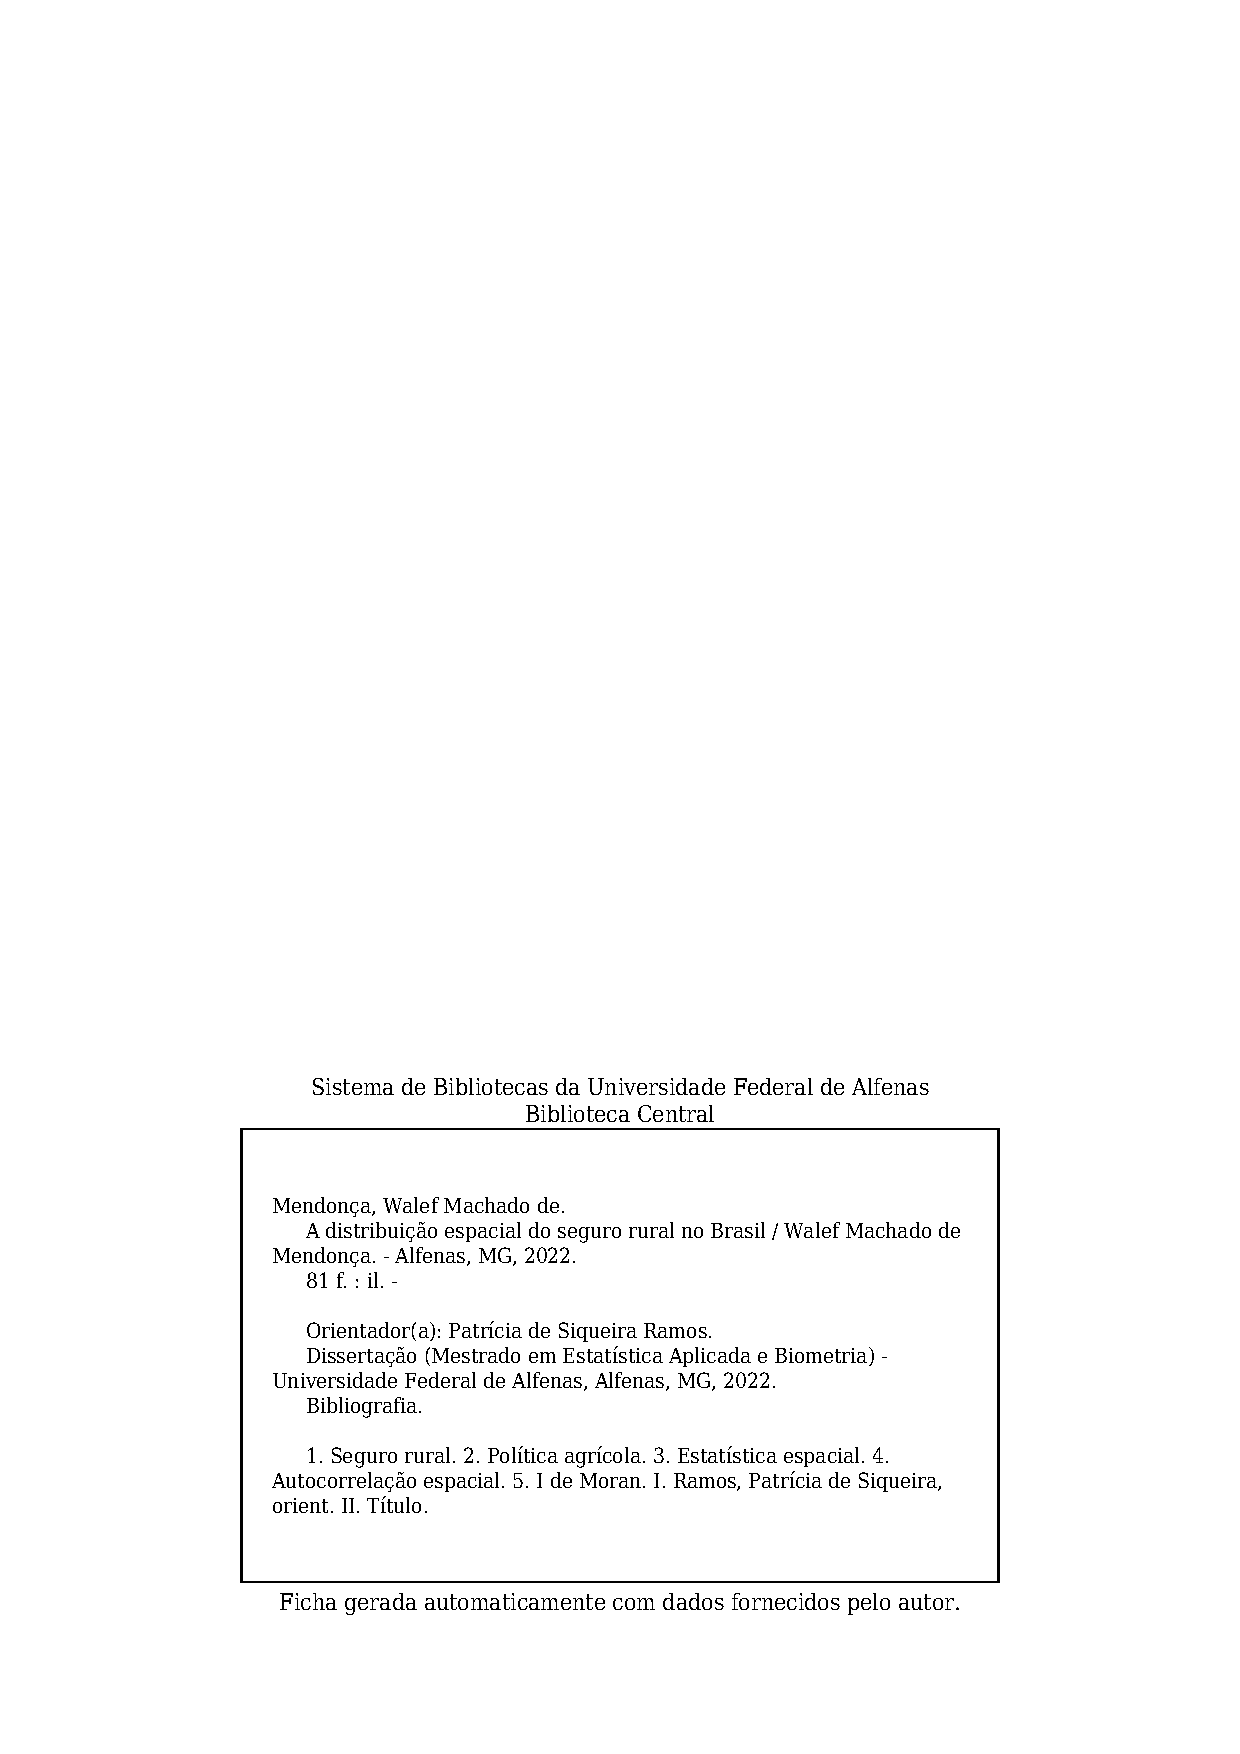
\includepdf[pages=1]{anexos/ficha_catalografica}

%\newpage
%\textcolor{white}{fantasma}

%\vfill
%\begin{center}
%\begin{singlespace}
%Dados Internacionais de Catalogação-na-Publicação (CIP) \\
%Sistema de Bibliotecas da Universidade Federal de Alfenas
%\vspace{-0.2cm}
%\end{singlespace}
%\end{center}
%\begin{center}
%\begin{boxedminipage}{12.8cm}
%\begin{singlespace}
%\begin{center}
%\hspace*{0.8cm}
%\begin{tabular}{p{11cm}}
%\vspace{0.5cm} \noindent{\teseauthorrev.}\\
%\hspace*{0.5cm} \tesetitle{} / \teseauthor.  -- Alfenas : UNIFAL, \teseyear.\\
%\hspace*{0.5cm} %\pageref{ultima} p. : il.
%\vspace{0.4cm}

%\hspace{0.5cm} Orientador: \teseorientador.\\
%\hspace{0.5cm} Dissertação (Mestrado em Estatística Aplicada e Biometria) -- Universidade Federal de Alfenas, \teseyear.\\
%\hspace{0.5cm} Bibliografia.

%\vspace{0.4cm}

%\hspace{0.8cm} .
%1. Análise espacial (Estatística). 2. Estatística agrícola. 3.
%Seguro rural. I. Ramos, Patrícia de Siqueira. II. Título. \\
%\multicolumn{1}{r}{}\\
%\multicolumn{1}{r}{}
%\end{tabular}
%\end{center}
%\end{singlespace}
%\end{boxedminipage}
%\vspace{0.2cm}
%\begin{singlespace}
%Ficha Catalográfica elaborada por -- \\
%Bibliotecária-Documentalista --
%\end{singlespace}
%\end{center}
%\pagebreak[4]

%=========================================================================================================
% página de aprovação
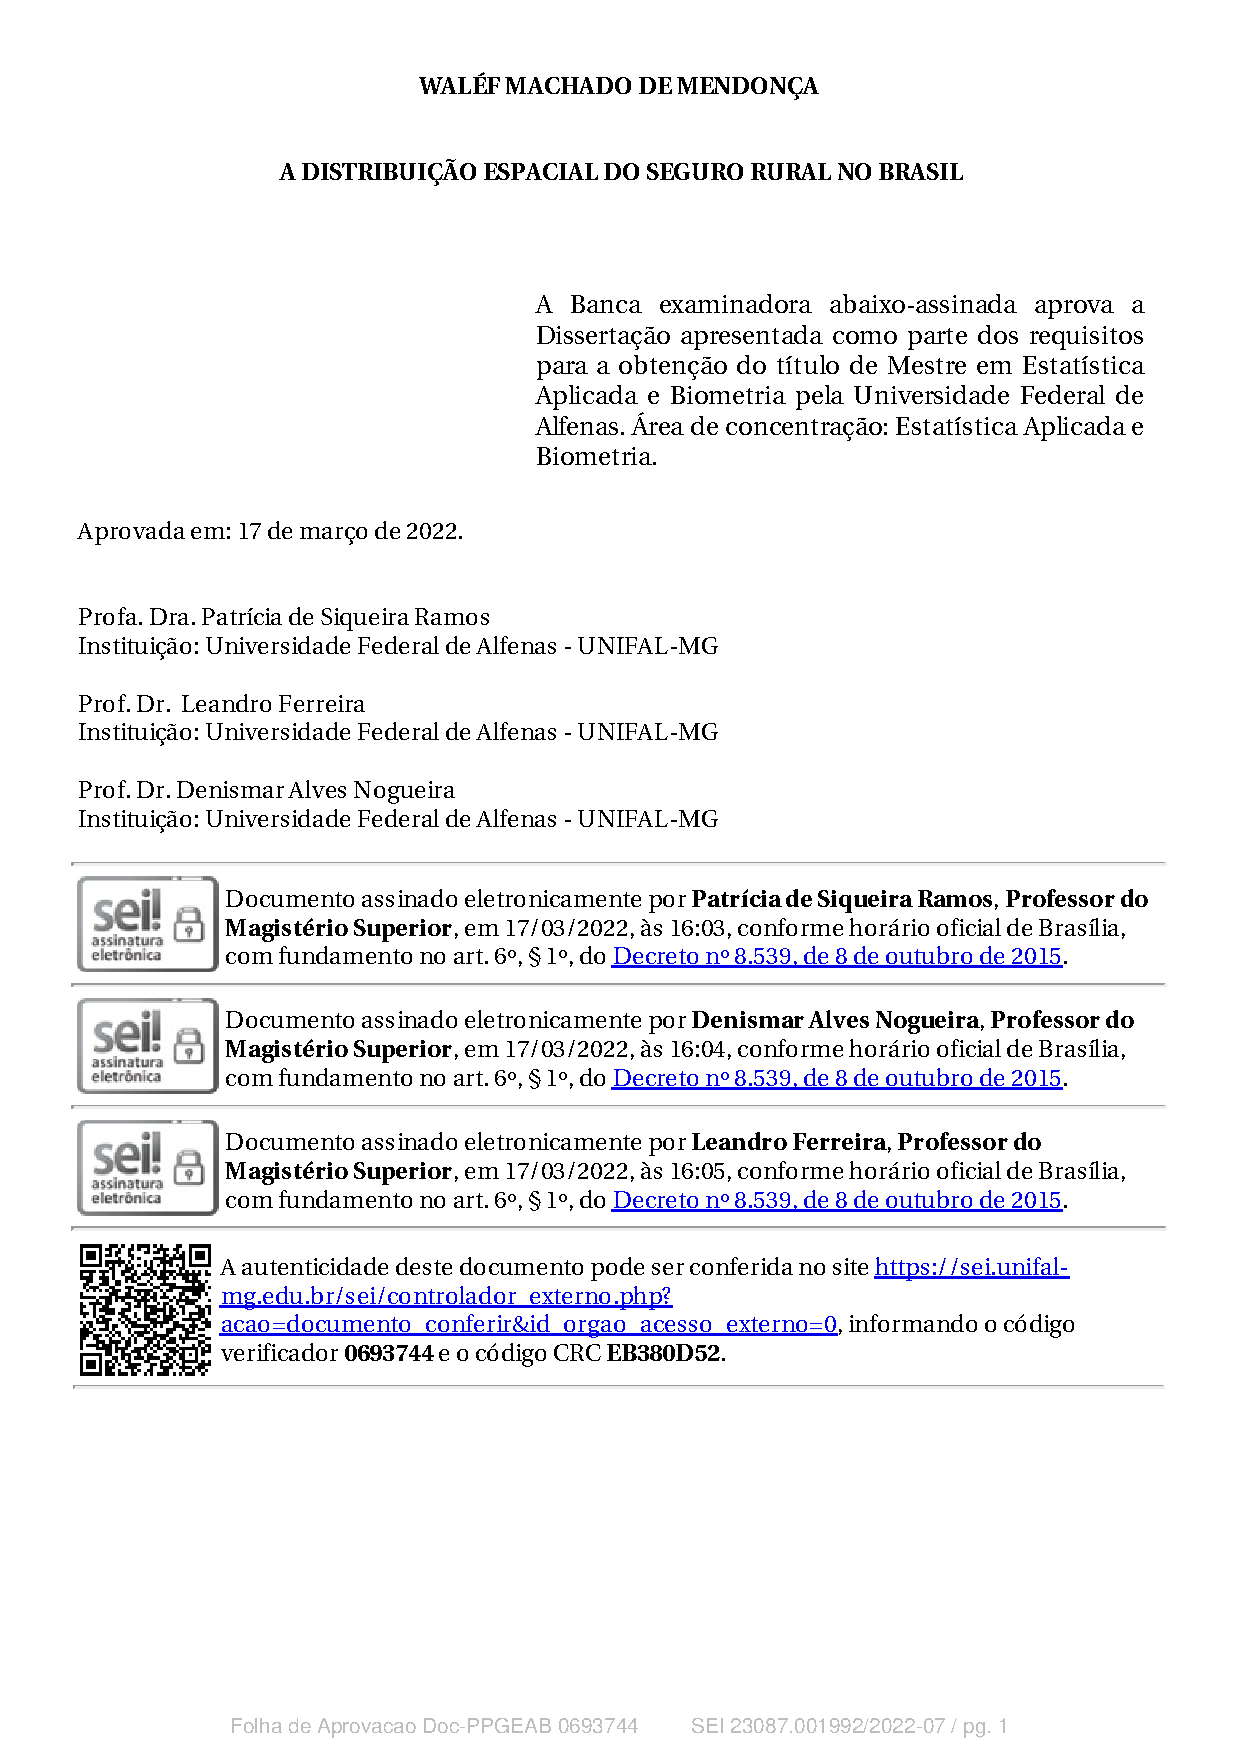
\includepdf[pages=1]{anexos/aprovacao_walef}

%\newpage
%\section*{}
%\vspace{-0.7cm} \centerline{\textbf{\teseauthorcap}}
%\vspace{1.4cm}
%\begin{singlespace}
%\begin{center}
%\textbf{\tesetitlecap}
%\end{center}
%\end{singlespace}
%\vspace{0.5cm}

%\begin{flushright}
%\begin{minipage}{9.6cm}
%\begin{quote}
%\begin{singlespace}
%A Banca examinadora abaixo-assinada, aprova a Dissertação apresentada como parte dos requisitos para obtenção do título de Mestre em Estatística Aplicada e Biometria pela Universidade Federal de Alfenas. Área de concentração: Estatística Aplicada e Biometria. Linha de pesquisa: Modelagem Estatística e Estatística Computacional.
%\end{singlespace}
%\end{quote}
%\end{minipage}
%\end{flushright}
%\vspace{1cm}

%\noindent\begin{tabular}{ll}
%Aprovado em XX de XXXX de 2022. \\
%\\
%\\
%Prof. Dra. \teseorientador & Assinatura:\\
%Instituição: Universidade Federal de Alfenas \\
%\\
%Prof. Dr. Leandro Ferreira & Assinatura:\\
%Instituição: Universidade Federal de Alfenas\\
%\\
%Prof. Dr. Denismar Alves Nogueira & Assinatura:\\
%Instituição: Universidade Federal de Alfenas\\
%\\


%\end{tabular}
%\begin{center}
%\begin{singlespace}
%%\vspace{0.8cm}
%\centerline{Prof. Dra. \teseorientador}
%\centerline{Orientadora}
%\vfill
%{\textbf{ALFENAS - MG\\ \teseyear}}
%\end{singlespace}
%\end{center}

% página em branco
%\newpage\null\thispagestyle{empty}\newpage

%=========================================================================================================
% dedicatória
\section*{}
\vspace{20cm}
\begin{flushright}

\textit{
\hspace{8cm} Aos meus pais, Adelvando e Dionísia, e a
\hspace{7cm} minha tia Cleonice, por todo amor e cuidado.}
\hspace{15cm}\textbf{Dedico este trabalho a vocês.}
\end{flushright}

% página em branco
%\newpage\null\thispagestyle{empty}\newpage

%===============================================================================
% agradecimentos

\newpage
\begin{center}
\textbf{AGRADECIMENTOS}
\end{center}
\vspace{0.5cm}

A maior parte dos ensinamentos que eu adquiri não foram através da análise de dados, sentado na frente de um computador, ou lendo pesquisas acadêmicas -- apesar de ter feito muito isso --, mas sim através da convivência com pessoas fantásticas cujas contribuições merecem algumas palavras de agradecimento. 

Nestes quase $7$ anos de graduação e pós-graduação na Universidade Federal de Alfenas eu tive o privilégio de estudar e trabalhar com pessoas que transformaram minha maneira de compreender o mundo e tornaram minha vida muito mais rica. 

Sou muito grato a todos os bons professores que pude conhecer na Unifal, tanto na graduação quanto no mestrado. Pude aprender um com cada um deles. 

Agradeço especialmente aos professores e amigos Patrícia Ramos e Lincoln Frias que, pacientemente, me acompanharam e apoiaram desde o início da graduação e que nunca deixarão de ser uma grande fonte inspiração em minha vida.

Agradeço também a generosidade dos professores Leandro Ferreira e Denismar Alves Nogueira. Os comentários e sugestões realizados durante o exame de qualificação e durante a defesa da dissertação contribuíram de forma decisiva para lapidar e direcionar o sentido do trabalho, além de proporcionarem reflexões para trabalhos futuros. 

Agradeço aos amigos que fiz na Unifal: Alice Duarte, Iris Rodrigues, Matheus Saraiva, Marcos Taroco, Poliana Benelli e Taylor Fidelis. O apoio dessas pessoas marcou profundamente minha formação intelectual e as minhas percepções com relação aos desafios da vida acadêmica. 

Sou muito grato também a todos os colegas que pude conhecer durante o mestrado. Agradeço especialmente o Giovani Festa e a Rafaela Gomes que tanto contribuíram para o meu aprendizado durante esses últimos dois anos. 

Não poderia deixar de agradecer também o constante apoio dos meus amigos Francisco Domingueti, Marcio Aloisio e Suzane Petruci. Nestes anos, que reforçaram a importância da proximidade espacial em todos os nossos relacionamentos, a presença dessas pessoas formaram os alicerces mais decisivos, através do apoio, compreensão, e orientações em todos os sentidos da minha vida.

Por fim, vale destacar que o presente trabalho foi realizado com apoio da Coordenação de Aperfeiçoamento de Pessoal de Nível Superior - Brasil (CAPES) - Código de Financiamento 001 

%===============================================================================
% epigrafe

\newpage
\section*{}
\vspace{16cm}


 
\setlength{\epigraphrule}{0pt}
\epigraph{
``Humans are good at discerning subtle patterns that are really there, but equally so at imagining them when they altogether absent.''}{Carl Sagan (1985)}

\setlength{\epigraphrule}{0pt}
\epigraph{
``In the face of ambiguity, refuse the temptation to guess''}{Tim Peters (2004)}


% página em branco
%\newpage\null\thispagestyle{empty}\newpage

%===============================================================================


%=========================================================================================================

\newpage
\thispagestyle{empty}

%% inclui resumo e abstract geral
%=========================================================================================================
% Resumo

\begin{singlespace}
\begin{center}
\section*{RESUMO}
\end{center}
As atividades agropecuárias se inserem em um contexto de adversidades que as colocam em situação diferenciada em relação aos riscos enfrentados pelos produtores. Tais atividades demandam grandes investimentos, o que faz com que sua atratividade esteja relacionada às formas existentes de gerenciamento de riscos. Uma das formas usuais de gerenciamento de risco neste setor é a contratação de seguro rural, uma vez que esta modalidade de seguro possibilita a recuperação da capacidade financeira do produtor na ocorrência de sinistros. Dessa forma, o objetivo da presente pesquisa é analisar a distribuição e a dinâmica espacial de variáveis relacionadas às apólices de seguro rural contratadas nos municípios brasileiros no período de 2006 a 2019. Para tanto, a dissertação foi dividida em dois artigos. No primeiro, o objetivo é avaliar a evolução das variáveis relacionadas ao seguro rural de forma individual. Para esse fim, inicialmente foi realizada uma análise descritiva da evolução das variáveis de apólices de seguro rural. Em seguida, foi empregada a Análise Exploratória de Dados Espaciais (AEDE), com o objetivo de identificar a existência de dependência espacial nas variáveis. Os resultados indicam que as maiores concentrações de apólices de seguro rural estão situadas nas regiões Sul e Centro-Oeste. Além disso, apesar de haver um aumento nas contratações de seguro rural, há também uma tendência de maior concentração espacial das apólices ao longo do período analisado. No segundo artigo, o objetivo é investigar a distribuição espacial do seguro rural nos municípios brasileiros no período de 2006 a 2019. Para alcançar tal objetivo, foi utilizada a Análise de Componentes Principais (ACP), com objetivo de reduzir a dimensionalidade dos dados. Os escores do primeiro componente principal foram  utilizados na Análise AEDE para investigar a presença de padrões de distribuição espacial de dados multivariados de seguro rural. Os resultados apontam que as maiores concentrações de apólices de seguro rural estão situadas nas regiões Sul e Centro-Oeste e há uma tendência de aumento na dependência espacial do seguro rural ao longo do período analisado. Em ambos os artigos foram utilizados dados dos Censos do seguro rural, compilados pelo Ministério da Agricultura, Pecuária e Abastecimento (MAPA) e dados com atributos geográficos do território disponíveis no endereço eletrônico do Instituto Brasileiro de Geografia e Estatística (IBGE).\\
\newline
\noindent {Palavras-chave:} Seguro rural. Política agrícola. Estatística espacial. Autocorrelação espacial. I de Moran.
\end{singlespace}


%=========================================================================================================
% Abstract

\newpage
\begin{singlespace}
\begin{center}
\section*{ABSTRACT}
\end{center}
Agricultural activities are inserted in a context of adversities that place them in a different situation in relation to the risks faced by producers. Such activities demand large investments, which makes their attractiveness related to existing forms of risk management. One of the most common forms of risk management in this sector is the contracting of Rural Insurance, since this type of insurance makes it possible to recover the producer's financial capacity in the event of accidents. Thus, the objective of this research is to analyze the distribution and spatial dynamics of variables related to rural insurance policies contracted in Brazilian municipalities from 2006 to 2019. For this purpose, the dissertation was divided into two articles. In the first, the objective is to evaluate the evolution of variables related to rural insurance individually. For this purpose, a descriptive analysis of the evolution of rural insurance policy variables was initially carried out. Then, the Exploratory Analysis of Spatial Data (ESDA) was used in order to identify the existence of spatial dependence in the variables. The results indicate that the highest concentrations of rural insurance policies are located in the South and Center-West regions. In addition, despite an increase in rural insurance contracts, there is also a trend towards greater spatial concentration of policies over the period analyzed. In the second article, the objective is to investigate the spatial distribution of rural insurance in Brazilian municipalities in the period from 2006 to 2019. To achieve this objective, Principal Component Analysis (PCA) was used in order to reduce the size of the data. The scores of the first principal component were and used for the ESDA to investigate the presence of spatial distribution patterns of multivariate rural insurance data. The results show that the highest concentrations of rural insurance policies are located in the South and Center-West regions and there is a tendency for an increase in the spatial dependence of rural insurance over the period analyzed. Both articles used data from the rural insurance Census, compiled by the Ministry of Agriculture, Livestock and Supply (MAPA) and data with geographic attributes of the Brazilian territory available on the website of the Brazilian Institute of Geography and Statistics (IBGE).\\
\newline
\noindent {Keywords:} Rural insurance. Agricultural policy. Spatial statistics. Spatial autocorrelation. Moran’s I

\end{singlespace}


%=========================================================================================================
% Sumário

\newpage


\begin{center}
\renewcommand{\listfigurename}{LISTA DE FIGURAS}
\begin{spacing}{1.4}
\listoffigures
%{
%\let\oldnumberline\numberline%
%\renewcommand{\numberline}{\figurename~\oldnumberline}
%\listoffigures 
%}
\thispagestyle{empty}
\end{spacing}
\end{center}

\newpage

\begin{center}
\renewcommand{\listtablename}{LISTA DE TABELAS}
\begin{spacing}{1.4}
%\listoftables
{
\let\oldnumberline\numberline%
\renewcommand{\numberline}{\tablename~\oldnumberline}
\listoftables 
}
\thispagestyle{empty}
\end{spacing}
\end{center}

\newpage

\begin{center}
\renewcommand{\contentsname}{\normalsize{SUMÁRIO}}
\begin{spacing}{1.4}
\tableofcontents
\thispagestyle{empty}
\end{spacing}
\end{center}


\newpage
\pagestyle{fancy}

\section{INTRODUÇÃO GERAL}

O agronegócio brasileiro tem se mostrado o único ramo da economia a apresentar crescimento no decorrer dos últimos anos \cite{guia_20}. Segundo cálculos realizados pelo Cepea (Centro de Estudos Avançados em Economia Aplicada), da Esalq/USP, em parceria com a CNA (Confederação da Agricultura e Pecuária do Brasil), o PIB do agronegócio brasileiro segue em expansão. Em 2019, a parcela do agronegócio brasileiro foi de  $20,5\%$  do PIB nacional. Já em 2020, o setor agropecuário brasileiro alcançou a participação de $26,6\%$ do PIB. Em valores monetários, o PIB do País totalizou R\$ $7,45$ trilhões em 2020, e a participação do agronegócio chegou a quase R\$ $2$ trilhões. 

Ainda segundo o relatório do Cepea, até o segundo trimestre de $2021$, o PIB do agronegócio brasileiro já havia acumulado um aumento de $9,81\%$ em relação ao mesmo período no ano anterior. Além disso, o relatório aponta que, ao se considerar o atual desempenho da economia brasileira, a participação do agronegócio nacional deve ficar em torno de $30\%$ do PIB em $2021$ \cite{cepea21}. 

Segundo dados dos censos agropecuários, entre $2006$ e $2017$, tanto a área total quanto a produção agrícola e pecuária vivenciaram crescimento. Neste período, houve um acréscimo de cerca de $5,8\%$ na área total dos estabelecimentos agropecuários (IBGE, 2019). De acordo com o Guia de Seguros Rurais, elaborado pela Comissão Nacional de Política Agrícola da Confederação da Agricultura e Pecuária do Brasil (CNA) e pelo Ministério da Agricultura, Pecuária e Abastecimento (MAPA), esse resultado advém do crescimento da área plantada das principais culturas e, de maiores investimentos em equipamentos e tecnologias \cite{guia_20}.

Dada a relevância do setor agropecuário na economia brasileira, é necessário destacar que este ramo possui características muito específicas com relação à dimensão dos riscos aos quais está sujeito \cite{burgo05}. Alguns riscos mais relevantes se devem, principalmente, às instabilidades climáticas e ameaças sanitárias que podem afetar a produção. Há também riscos devidos à razões de mercado, como variações das taxas de câmbio e juros, ou a condições ligadas ao ambiente de negócios, tais como, alterações em marcos regulatórios e em políticas públicas. Todos esses fatores geram variações na renda do setor e, mesmo em anos de crescimento das safras, eventos climáticos de alcance regional podem atingir os produtores, e causar perdas expressivas. Dessa forma, é necessário que sejam empregadas políticas de apoio à gestão de riscos \cite{brasil21}. 

Uma gestão de riscos apropriada tem potencial de afetar de forma positiva a estabilidade da renda do produtor e sua própria permanência no setor agropecuário. O gerenciamento de riscos agropecuários pode ocorrer de diversas maneiras, no entanto, a contratação de seguro é uma das medidas mais comuns. O seguro rural é uma importante ferramenta de mitigação de riscos e proteção da renda. Esta modalidade de seguro atua no sentido de amenizar as perdas e possibilitar a recuperação da capacidade financeira do produtor rural em caso de ocorrência de sinistros \cite{brasil19b}.  

Nesse sentido, este estudo tem  o intuito de fornecer informações para o debate de aperfeiçoamentos no sistema de seguro rural brasileiro, de forma a contribuir para uma agricultura mais eficiente e com menores riscos para o produtor rural. Para tanto, a presente pesquisa foi dividida em dois artigos. No primeiro deles, o intuito é realizar uma análise exploratória da evolução das variáveis relacionadas ao seguro rural entre os anos de $2006$ e $2019$. Para esse fim, foi realizada uma análise descritiva da evolução das variáveis de apólices de seguro rural. 

O segundo artigo, por sua vez, tem como objetivo investigar a distribuição espacial de dados multivariados do seguro rural nos municípios brasileiros entre os anos de $2006$ e $2019$. Para tanto, busca-se investigar se, no Brasil, as variáveis de seguro rural se distribuem de forma aleatória no espaço ou se há padrões de distribuição espacial. Além disso, por meio da análise da distribuição espacial do seguro rural no período, busca-se identificar se há regiões que tiveram alterações significativas no número de contratações de seguro. 

Para alcançar tais objetivos, o segundo artigo faz uso da Análise de Componentes Principais (ACP), com objetivo de reduzir a dimensionalidade dos dados e incorporar aos escores do primeiro componente principal informação das variáveis originais. Para mais, utiliza-se a Análise Exploratória de Dados Espaciais (AEDE), aplicada aos escores do primeiro componente principal, com o objetivo de investigar a presença de padrões de distribuição espacial.

Em ambos os artigos, foram utilizados dados dos Censos do seguro rural, compilados pelo Ministério da Agricultura, Pecuária e Abastecimento (MAPA) e dados com atributos geográficos do território brasileiro disponíveis no endereço eletrônico do Instituto Brasileiro de Geografia e Estatística (IBGE).

\newpage
\section{REFERENCIAL TEÓRICO}

O objetivo dessa seção é fazer uma apresentação do sistema de seguro rural e como ele se estruturou no Brasil. Por fim, são apresentados aspectos da análise espacial e da análise multivariada. 

\subsection{O SEGURO RURAL}

O gerenciamento de riscos agropecuários pode ser efetuado de diversas formas, no entanto, a contratação de seguro rural é uma das formas mais usuais. Essa modalidade de seguro é um dos mais importantes instrumentos de política agrícola, pois possibilita que o produtor rural se proteja e mantenha sua capacidade financeira no caso de ocorrência de perdas decorrentes, principalmente, de fenômenos climáticos adversos \cite{susep21_g}. Não obstante, o seguro rural é mais abrangente e cobre não só as atividades agrícolas, mas também oferece cobertura para a pecuária, para o patrimônio do produtor, seus produtos, o crédito para comercialização desses produtos e até mesmo oferece seguro de vida aos produtores \cite{cnsp16_g}. 

Desse modo, o objetivo do seguro rural é proporcionar coberturas que, ao mesmo tempo, atendam ao produtor e a sua produção, à geração de garantias a seus financiadores, investidores, parceiros de negócios, ou seja, todos interessados na maior diluição possível dos riscos das atividades agropecuárias. Dessa forma, o seguro rural propicia um ambiente mais favorável ao desenvolvimento das atividades agropecuárias pois proporciona a garantia do fluxo de renda, favorece um aumento da área plantada, facilita a obtenção de financiamento e possibilita o compartilhamento do risco da agropecuária com outros agentes e setores econômicos \cite{susep21_g}. 

No entanto, é importante destacar que a adesão ao seguro rural no Brasil ainda é muito baixa. Segundo dados do Ministério da Agricultura e Pecuária e Abastecimento, em 2018, apenas $42.376$ produtores rurais brasileiros adotaram o seguro como forma de gerenciar os riscos agropecuários \cite{brasil21}. Ao se considerar os dados do Censo Agropecuário de 2017, que apontam a existência de cerca de  $5.073.324$ de estabelecimentos  agropecuários no Brasil, é possível depreender que o percentual de estabelecimentos que utilizam seguro rural é consideravelmente limitado \cite{ibge19}.

A baixa adesão ao seguro rural se deve a diversos problemas relacionados ao funcionamento do mercado. Destacam-se problemas como os elevados investimentos e custos administrativos, a possibilidade de riscos catastróficos, a forte influência do risco moral e da seleção adversa na formação das carteiras, como fatores que limitam a eficiência da iniciativa privada na oferta de produtos \cite{brasil19b}. Segundo Ozaki (2010), outro fator que atua no sentido de limitar a atuação das seguradoras no ramo do seguro rural é a qualidade e quantidade de informações disponíveis. 

Nesse contexto, as próximas seções apresentam uma breve discussão dos modelos de seguro rural implantados em outros países, como Estados Unidos, Canadá e Espanha, e o modelo que vem se  desenvolvendo no Brasil.


\subsubsection{O seguro rural em outros países}

Ao analisar as principais experiências internacionais, Ferreira e Ferreira (2009) comparam o desenvolvimento do seguro rural no Brasil com as experiências desse ramo de seguro nos Estados Unidos e no Canadá. Tanto no Brasil quanto nos outros países analisados, Ferreira e Ferreira (2009) apontam que o maior desafio da atuação do setor público é encontrar uma forma de fomentar o seguro rural que não crie distorções na produção e estimule a perda de produtividade. No entanto, segundo Ferreira e Ferreira (2009), a participação do governo é fundamental e deve garantir a sustentabilidade do seguro rural no caso de ocorrência de eventos catastróficos de forma a assegurar a estabilidade social dos agricultores e demais participantes do sistema. Além disso, destaca-se que o grande obstáculo, para a atuação do setor público, é ser capaz de conservar a renda dos agricultores sem comprometer o orçamento público, de maneira que os programas de seguro rural sejam autossustentáveis \cite{ferreira09_g}.  

Segundo Fornazier, Souza e Ponciano (2012), ao analisar as experiências e modelos de seguro rural adotados no Brasil, Espanha e EUA, mesmo entre os países desenvolvidos, foi necessário muitos anos para estabelecer os atuais modelos. A Espanha levou 25 anos para desenvolver seu atual modelo de seguro agrícola e, nos EUA, o desenvolvimento do atual modelo de seguro rural levou cerca de quase 70 anos \cite{ozaki06_g}.

% Em países onde os recursos públicos são escassos, como o Brasil, é pouco provável que ocorra alguma forma de subsídio direto como nos EUA, ao contrário, salienta-se a utilização de incentivos indiretos. Esse é o caso da Argentina, onde a Oficina de Riesgo Agropecuario (ORA) considera que os efeitos do clima, os rendimentos, os custos e a variabilidade de preços são fundamentais para um diagnóstico e manejo adequado do risco agrícola. Assim, o governo Argentino desenvolveu um modelo de Manejo Integrado do Risco Agropecuário que combina as seguintes estratégias: i) avaliação orientada para a sistematização e análise da informação necessária para obter conclusões precisas sobre o risco; ii) redução do risco pela minimização do impacto previamente avaliado (REDPA, 2004). 

% Em função desse enfoque a ORA tem como missão as seguintes atividades: i) gerar, atualizar, e publicar os Mapas de Riesgo Agro-Climáticos, baseados no tratamento sistemático de variáveis climáticas e seus impactos sobre a atividade agropecuária; ii) publicar mensalmente indicadores sobre os fenômenos climáticos de grande escala a exemplo do fenômeno El Niño Oscilação Sul 12 ; iii) desenvolver e oferecer ferramentas de análise de risco econômico por meio dos Portafolios Eficientes 13 ; iv) construir, publicar e promover a adoção dos Portafolios Óptimos como uma estratégia de redução do risco baseada na diversificação de atividades; v) difundir informação atualizada da evolução de preços e conscientizar os atores da importância dos riscos de mercado e das vantagens de adotar um esquema de coberturas; vi) desenvolver novas áreas técnicas para estudo de outros riscos relacionados, a exemplo do risco em atividades florestais; vii) analisar e promover o desenvolvimento de novas opções de comercialização para o setor agrícola; viii) implementar um plano de ação dirigido a expandir o mercado de seguros agropecuários de modo de alcançar o maior número de produtores, nas distintas zonas do país e nas diferentes atividades agropecuárias; e ix) promover a assistência técnica e assessorar a implementação de políticas relacionadas com o manejo do risco agropecuário e o desenvolvimento do mercado de seguros aos Governos Provinciais que solicitem (REDPA, 2004).

% VIEIRA JUNIOR, Pedro Abel \textit{et al.}. Dimensões e perspectivas do Seguro Rural: o caso brasileiro e algumas experiências internacionais. 2008.

Nesse sentido,  a literatura aponta que é necessário que o poder público interfira no mercado, ou atuando diretamente como seguradora, ou criando programas que estimulem o mercado de produtos de seguro rural. No Brasil, um dos mecanismos adotados foi o programa de subvenção ao prêmio de seguro rural, que será discutido mais adiante. 

\subsubsection{O seguro rural no Brasil}

%Primeiro seguro rural e primeiras "iniciativas" de seguro rural
No Brasil, as primeiras iniciativas de implementar o seguro rural ocorreram em meados da década de $1930$ e desenvolveram-se principalmente nas esferas estaduais. Em $1939$, o Estado de São Paulo determinou a criação de um seguro obrigatório contra o granizo na produção de algodão \cite{maia11}. Segundo Silva, Teixeira e Santos (2014), os resultados do seguro para a proteção da lavoura algodoeira em São Paulo influenciaram a criação de novos programas como a Carteira de Seguro Agrícola contra Granizo para a Viticultura, criada em $1948$, e a Carteira de Seguro Agrícola contra Geada para Horticultura instituída em $1964$

O trabalho de Silva, Teixeira e Santos (2014) também destaca o seguro para granizo, criado no final da década de $1940$ no Instituto Rio-Grandense do Arroz (Irga), e o seguro criado pela Associação dos Fumicultores do Brasil (Afubra), que buscava indenizar com recursos próprios os produtores de fumo nos estados de Santa Catarina e Rio Grande do Sul.

No âmbito federal, em $1948$, foi criado o Instituto de  Resseguros do Brasil (IRB), para diminuir os danos de eventos adversos e garantir maior estabilidade aos produtores rurais \cite{silva14}. Além disso, também foi criada pelo Governo Federal, em $1954$, a Companhia Nacional de Seguro Agrícola (CNSA) e o Fundo de Estabilidade do Seguro Agrário. Ademais, Maia,  Roitman e de Conti (2011) evidenciaram que a estruturação e gestão dos seguros da CNSA ficaram sob responsabilidade do IRB. Contudo, as atividades da CNSA foram encerradas em $1996$, devido, segundo Gemignani (2000), ao insucesso em difundir o seguro rural de forma a possibilitar sua exploração econômica \cite{maia11, silva14}.

Em $1966$ e $1967$, são instituídos o Decreto-Lei nº $73$ e o Decreto nº $60.459$, que estabelecem as bases legais para as atividades de seguro e a criação do Sistema Nacional de Seguros Privados (SNSP). O decreto de $1967$ também criou o Fundo de Estabilidade do Seguro Rural (FESR), cujos recursos eram geridos pelo IRB e o objetivo principal era assegurar a estabilidade das operações de seguro e fornecer uma cobertura adicional para os riscos de sinistro \cite{silva14}

A Resolução nº $5$ do Conselho Nacional de Seguros Privados, instituída em $1970$, teve um importante papel na definição das modalidades de seguros agrários. Nesta Resolução, foi definido o seguro agrícola, que fornece cobertura contra perdas decorrentes de fenômenos meteorológicos, doenças e pragas, o seguro pecuário que fornece cobertura para morte de animais causadas por doenças ou acidentes, assim como, o seguro de benfeitorias e produtos agropecuários. Por fim, a Resolução nº $5$ também estabelece o seguro de crédito, que cobre incapacidade de pagamentos de compradores dos produtos agropecuários \cite{silva14}.

%Criação do proagro
Apesar das diversas ações do Governo Federal, o seguro rural se desenvolveu de forma lenta e restrita à uma pequena parcela da produção, o que motivou a criação do Programa de Garantia da Atividade Agropecuária (Proagro), através da Lei nº $5.969$, de $11$ de dezembro de $1973$ \cite{silva14}. Inicialmente, sob a responsabilidade do Banco Central, o Proagro passou a vincular o seguro rural às operações de crédito agropecuário e utilizou emissões monetárias para pagamentos de sinistros. Segundo Maia, Roitman e De Conti (2011), o sistema de financiamento do Proagro gerou déficits que motivaram diversas modificações no Programa, sendo ainda um dos mais importantes instrumentos para a gestão de riscos na agricultura no Brasil \cite{maia11}.

%Criação do PSR
A partir de $2003$, o Governo Federal passou a adotar uma política de subvenção por meio do Programa de Subvenção ao Prêmio do Seguro Rural (PSR), instituído por meio da Lei nº $10.823$ de $19$ de dezembro de $2003$ e do Decreto nº $5.121$ de $2004$ \cite{brasil18}. Este programa busca, assim como ocorre em países europeus e nos Estados Unidos, conceder subvenção econômica ao valor do prêmio do seguro rural contratado com seguradoras autorizadas.

\subsubsection{Programa de Subvenção ao Prêmio do Seguro Rural}

Segundo o Decreto nº $5.121$ de $2004$, o PSR tem a finalidade de subsidiar parte do prêmio do seguro rural, de forma a assegurar a função do seguro rural como mecanismo de estabilidade da renda do produtor, além de suscitar a aplicação das tecnologias adequadas para os empreendimentos agropecuários \cite{guia_20}. Tal política do governo busca tornar o seguro rural mais acessível aos agricultores, dividindo os custos de aquisição da apólice entre o governo e os produtores. 

A operacionalização do PSR é feita pelo Ministério da Agricultura, Pecuária e Abastecimento (MAPA), envolve os produtores rurais, que devem fazer a contratação do seguro rural diretamente com as seguradoras habilitadas pela Superintendência de Seguros Privados (Susep) e cadastradas no MAPA. Desta forma, para obter os recursos do programa, os produtores devem contratar a apólice e requerer a subvenção do governo federal. O governo federal, por sua vez, repassa para as seguradoras habilitadas, um percentual do prêmio do seguro contratado, resultando da redução do valor a ser pago pelo produtor rural \cite{silva14}.

O valor concedido como subvenção ao prêmio do seguro rural leva em conta algumas características como a modalidade do seguro, o tipo de cultura e o tipo de cobertura. As técnicas de execução e prioridades da política do PSR são estabelecidas pelo Comitê Gestor Interministerial do Seguro Rural (CGSR). Com o objetivo de fiscalizar a gestão do programa, este comitê é formado pelo MAPA, que é responsável pela coordenação, e por representantes do Ministério da Economia (ME) e da Superintendência de Seguros Privados (Susep) \cite{brasil21_2} 

Em análise à evolução do PSR, Macedo, Pacheco e Do Espírito Santo (2013) apontam que, ao longo do período de 2006 a 2010, a agenda da política agropecuária brasileira vivenciou uma evolução qualitativa, através da introdução do PSR. No entanto, os recursos destinados à subvenção do prêmio de seguro rural no orçamento federal ainda eram inferiores aos necessários para a cobertura de percentuais da produção agropecuária similares aos alcançados em outros países. Dessa forma, os recursos federais disponibilizados precisavam ser aperfeiçoados, para que alcançassem taxas representativas de cobertura no seguro rural \cite{macedo13_g}. 

Ao investigar a participação do PSR na universalização do acesso ao seguro rural, Silva, Teixeira e Santos (2014) apontam que os dados podem levar à falsa conclusão de que as metas de ampliação do seguro pelo PSR foram atingidas em nível nacional no período de 2005 a 2012. Não obstante, quando os dados foram desagregados por região, observou-se uma concentração das subvenções na região Sul desde a implantação do PSR. Desse modo, os objetivos do programa foram cumpridos de forma parcial, pois, apesar de ter ocorrido uma ampliação do seguro rural, esta ampliação ocorreu de forma concentradora \cite{silva14}. 

Em face da relevância do setor agrícola para a economia brasileira, é possível compreender que o seguro rural e o PSR são importantes ferramentas de gestão de risco e que contribuem para uma agricultura mais eficiente e com menores riscos para o produtor rural. O PSR, em especial, opera como uma forma de estimular a aquisição das apólices de seguro rural, buscando induzir o uso de tecnologias apropriadas e modernizando a gestão do empreendimento agropecuário. 

\subsubsection{O zoneamento agrícola}

Conforme apresentado no Guia de Seguros Rurais (2020), o PSR tem como condicionalidade, para o recebimento da subvenção, o cumprimento dos indicadores do zoneamento agrícola de risco climático (ZARC). O ZARC faz um levantamento do período de plantio das culturas por município e leva em consideração características como o tipo de solo e o clima da região. Dessa forma, o ZARC busca evitar que eventos climáticos adversos ocorram durante as fases em que as culturas se encontram mais vulneráveis e, com isso, minimizar as perdas agrícolas \cite{guia_20}.

Como apresentado por Rossetti (2001), o  zoneamento agrícola de risco climático (ZARC) é um projeto que busca o desenvolvimento de estudos de regionalização dos eventos climáticos adversos no Brasil, com objetivo de minimizar as perdas da produção agrícola. Além disso, o zoneamento agrícola busca disponibilizar ao produtor rural métodos para mitigar os riscos climáticos. Segundo Rossetti (2001), os resultados demonstraram que o Zoneamento tem beneficiado o setor agropecuário brasileiro, principalmente no que diz respeito à redução das perdas provocadas por eventos climáticos e ao aumento da produtividade das lavouras zoneadas.

Dessa forma, o zoneamento agrícola integra uma ferramenta relevante para o gerenciamento dos riscos pelo produtor e pelas seguradoras. Desse modo, a concessão da subvenção ao prêmio de seguro pelo programa PSR se dá apenas quando há o cumprimento, pelo produtor rural, das recomendações estabelecidas pelo zoneamento agrícola de risco climático do MAPA. Nas situações em que não há o zoneamento de risco climático realizado pelo MAPA para alguma região ou cultura, a seguradora pode empregar zoneamentos de outras instituições oficiais de pesquisa que considerem critérios probabilísticos na determinação das datas de plantio e riscos das culturas \cite{santos16}. 

% Dependência espacial
Ao analisar a correlação espacial de dados de produtividade das culturas de milho e soja no Estado do Paraná entre 1990 e 2002, Ozaki (2008) aponta que há um padrão de dependência espacial nos dados e, dessa forma, as unidades seguradas não podem ser consideradas espacialmente independentes. Além disso, Ozaki (2008) destaca que, a presença de dependência espacial implica em sérias consequências no mercado de seguros agrícolas, pois o risco de insolvência das seguradoras frente aos segurados é grande, na ocorrência de um evento climático extremo.  Nesse sentido, portanto, as seguradoras devem se atentar a estratégias que possibilitem uma diversificação geográfica e a concentração de riscos em determinadas regiões deve ser evitada \cite{ozaki08_g}. 

Outro estudo que buscou analisar a dependência espacial do seguro rural no Brasil no ano de 2017, foi apresentado por Biazoli, Ramos e Frias (2020). Segundo os autores, foi possível observar que as apólices de seguro rural não se distribuíam de forma aleatória pelo território brasileiro e foi possível detectar a formação de aglomerados espaciais do seguro rural para nos estados da região Sul do Brasil. % \cite{biazoli20_g}

\subsection{ANÁLISE ESPACIAL}  
	
A análise espacial consiste em um conjunto de métodos capazes de mensurar propriedades e relacionamentos de acordo com a localização espacial de determinado fenômeno, buscando incorporar o espaço à análise. Dessa forma, antes de partir para a modelagem, é comumente  realizada a análise exploratória dos dados, buscando identificar os padrões de dependência espacial no fenômeno em questão \cite{camara04_g}.

A análise espacial é capaz de incorporar alguns fenômenos como a dependência espacial e a heterogeneidade espacial. A ocorrência da dependência espacial pode ser retratada pela Primeira Lei da Geografia, ou Lei de Tobler. Esta lei, enunciada em $1970$ pelo geógrafo Waldo Tobler, diz que tudo depende de tudo, mas coisas próximas estão mais relacionadas entre si do que coisas mais distantes. Dessa forma, a dependência espacial corresponde no fato de que o valor de uma variável em uma determinada região depender do valor desta mesma variável em regiões geograficamente próximas \cite{almeida12_g}.
	
Ainda segundo Almeida (2012), processos temporais possuem relações diferentes dos processos espaciais. Nos processos temporais, o valor de uma variável qualquer no tempo $t$ é influenciado pelo valor da variável no tempo $t-1$, mas o inverso não ocorre. Diferentemente desse tipo de processo, nos  processos espaciais têm-se a multidirecionalidade nas relações entre as regiões, ou seja, o valor da variável na região $i$ depende do valor na região $j$, e a região $j$ depende da região $i$ em relação ao valor da mesma variável.
	
%Heterogeneidade Espacial
	
Outro fenômeno espacial que deve ser incorporado à análise, é a heterogeneidade espacial. Tal fenômeno refere-se à variação nos relacionamentos entre as variáveis ao longo do espaço. Em geral, podem-se esperar diferentes relacionamentos em cada uma das unidades espaciais, ou seja, podem haver diferentes respostas, dependendo da localidade ou da escala espacial adotada no estudo. 
	
Faz-se necessário destacar que os dados espaciais apresentam alguns problemas que podem ser prejudiciais à análise. Além da heterogeneidade espacial e da dependência espacial, pode-se mencionar problemas como a falácia ecológica, o problema da unidade de área modificável, o efeito de beirada e a influência de \textit{outliers} espaciais. 
	
Segundo Almeida (2012), a falácia ecológica refere-se aos erros que ocorrem ao deduzir o comportamento do indivíduo através da análise de dados agregados. Almeida (2012) argumenta que há razões para inferir, ainda que parcialmente, comportamentos individuais por meio de dados agregados. Uma situação possível é quando alguns comportamentos individuais são influenciados pelo comportamento do grupo. No entanto, via de regra, as conclusões a respeito de comportamento individual devem se basear primordialmente em dados individuais. 

A ausência de dados individuais, ou o fato de unidades agregadas serem o foco da análise, torna necessário a utilização de informações espaciais agregadas. O uso dessas informações pode conduzir ao problema de unidade de área modificável, ou MAUP (do inglês \textit{modifiable areal unit problem}). Esse problema diz respeito às consequências ocasionadas pelas diversas maneiras de se delimitar as regiões em análise. 
	
Segundo Haining (2003), o MAUP apresenta dois efeitos distintos: efeito de escala e partição. O primeiro deles se relaciona à escala da análise, ou seja, ao número de subáreas em que a região de estudo foi particionada. O número de partições determina também o tamanho de cada unidade espacial nas quais os eventos são observados podendo influenciar o resultado de estatísticas. O segundo efeito diz respeito a forma das partição das unidades, ou seja, como as  áreas estão divididas, mantendo-se constante o número de áreas.
	
Por sua vez, o efeito de beirada ocorre em virtude da possibilidade da dependência espacial ir além das fronteiras da área de estudo, de forma que o valor da variável analisada possa depender de unidades espaciais que não a compõe \cite{anselin88_g}. Segundo Almeida (2012), este efeito afeta a  inferência estatística de modelos de processos espaciais. Além disso, por terem um menor número de regiões vizinhas, as regiões da fronteira também oferecem menos informações para a construção de valores médios, como por exemplo, as defasagens espaciais.
	
Como forma de mitigar o efeito beirada, Griffith (1983) propôs a criação de vizinhos artificiais para as regiões de fronteira através de suas replicações do mapa. Porém, como destacado por Darmofal (2006) a dúvida consiste em saber se tais vizinhos artificiais realmente apresentam interação espacial com a região. Outra solução apontada por Almeida (2012), seria estender a área de estudos, considerando adicionalmente uma zona ao longo de toda a fronteira.
	
%Outliers e pontos de alavancagem
A existência de \textit{outliers} espaciais ocorre em razão da dissimilaridade dos valores de uma variável em relação ao conjunto de valores dessa mesma variável das regiões vizinhas (HAINING, 2003). No caso, os \textit{outliers} espaciais são definidos como valores extremos com relação a suas localizações geográficas. 

Os \textit{outliers} espaciais, assim como os pontos de alavancagem, podem emergir do processo de obtenção dos dados, ou podem realmente sinalizar a presença de valores extremos e retratar atributos reais do fenômeno em estudo. Dessa forma, a existência de \textit{outliers} espaciais deve demandar uma investigação mais diligente \cite{almeida12_g}.
	
\subsubsection{Matriz de ponderação espacial} \label{W_matrix_2}
	
A matriz de ponderação espacial, ou matriz de pesos espaciais, tem como propósito representar estruturas espaciais decorrentes das interações de um fenômeno em estudo \cite{almeida12_g}.
Cada entrada em uma matriz de ponderação espacial representa a conexão entre duas regiões e é denominada peso espacial. A matriz de ponderação espacial, com dimensão $n \times n$, geralmente é denotada por $\boldsymbol{W}$: 
	
\begin{align*}
	\boldsymbol{W} =
    \left[
    \begin{array}{cccc}
        w_{11} & w_{12} & \dots & w_{1n} \\
        w_{21} & w_{22} & \dots &w_{2n} \\
        \vdots & \vdots & \ddots & \vdots \\
        w_{n1} & w_{n2} & \dots & w_{nn}\\
    \end{array}
    \right],
\end{align*}
	
\noindent em que $n$ é o número de regiões analisadas. Cada elemento $w_{ij}$ descreve uma medida de vizinhança entre as áreas $i$ e $j$ \cite{camara04_g}.
	
Existem dois problemas relacionados à determinação da matriz de ponderação espacial a ser utilizada. O primeiro está relacionado ao fato de que, muitas vezes a escolha da matriz $\boldsymbol{W}$ é arbitrária, pois não existe teste formal para sua escolha. O segundo problema, está relacionado a sensibilidade dos resultados à escolha da matriz. Portanto, a definição da matriz de ponderação espacial tem grande importância e deve levar em consideração uma fundamentação teórica \cite{almeida12_g}. 
	
É comum a utilização de atributos físicos e geográficos para estabelecer distâncias entre as regiões. Geralmente são utilizados critérios como a vizinhança, o tempo de deslocamento  ou a distância geográfica entre as unidades. Porém, é possível que as distâncias entre as regiões busquem representar mais aspectos socioeconômicos do que geográficos, como no caso de modelos espaciais aplicados a políticas públicas \cite{tyszler06_g}. 

Uma matriz de ponderação espacial por contiguidade leva em consideração, em sua definição, as fronteiras físicas em comum entre duas regiões. Na matriz de ponderação por contiguidade binária às regiões que apresentam relação de vizinhança, é atribuído ao elemento correspondente na matriz o valor $1$, caso contrário, é atribuído o valor $0$. Formalmente, tem-se:
	
\[
w_{ij} = 
	\begin{cases}
    	\text{1,} & \quad\text{se $i$ e $j$ são contíguos}, \\
	    \text{0,} & \quad\text{se $i$ e $j$ não são contíguos.}\\
	\end{cases}
\]
\\
	
Além disso, por convenção, assume-se que  $w_{ij} =  0$, para todo $i = j$, ou seja, uma região não é considerada vizinha de si mesma. O conceito de fronteira geográfica pode apresentar diferentes definições ao se observar um mapa. Como forma de ilustrar as definições de fronteira, comumente, utiliza-se o movimento de peças em um tabuleiro de xadrez \cite{almeida12_g}. 

Algumas das diferentes convenções de contiguidade são apresentadas na Figura \ref{contiguidade_2}. São representadas três diferentes convenções: rainha (\textit{queen}), torre (\textit{rook}) e bispo (\textit{bishop}). Na convenção de tipo rainha, além das regiões que fazem fronteira com a região $A$, os vértices são considerados vizinhos. Na convenção torre, apenas as regiões que fazem fronteira com a região são consideradas vizinhas de $B$. Na convenção bispo, apenas os vértices são considerados vizinhos da região $C$.
	
\begin{figure}[H]
	\centering
    \caption{Convenções de contiguidade$\quad\quad$}\label{contiguidade_2}
	\small
	\subfloat[Rainha\label{fig_queen_2}]{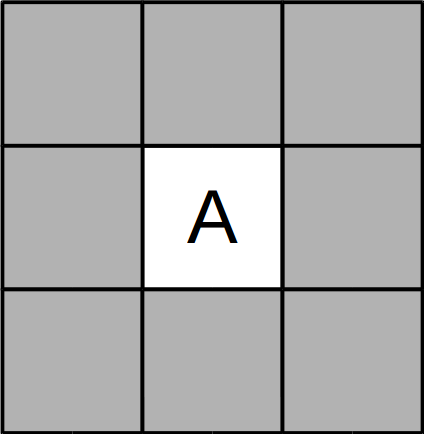
\includegraphics[width=0.15\textwidth]{figuras/cont_queen.png}}\hspace{0.2cm}
	\subfloat[Torre\label{fig_rook_2}]{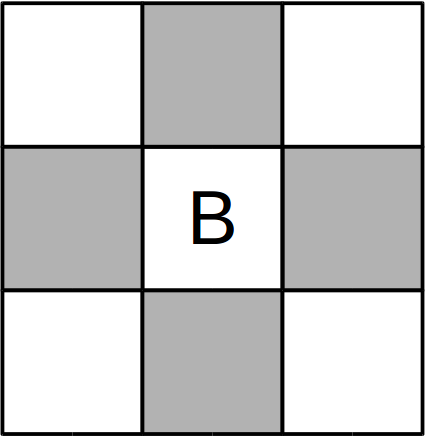
\includegraphics[width=0.15\textwidth]{figuras/cont_rook.png}}\hspace{0.2cm}
	\subfloat[Bispo\label{fig_bishop_2}]{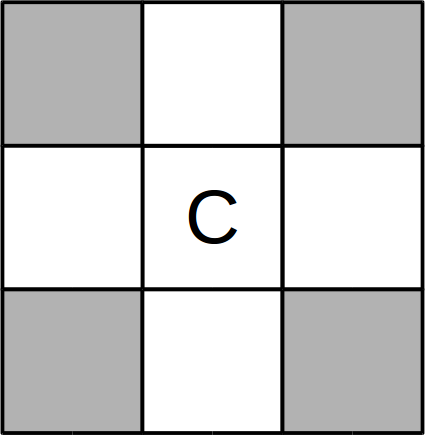
\includegraphics[width=0.15\textwidth]{figuras/cont_bishop.png}}\\
    %\small \textsuperscript {Fonte: Elaboração própria}
    \parbox{\dimexpr\linewidth-8.3cm}{\raggedright
    \strut \textsuperscript{Fonte: Elaboração própria}\strut}
\end{figure}
	
Faz-se necessário salientar que a matriz de contiguidade binária é simétrica, ou seja, se duas regiões quaisquer $i$ e $j$ compartilham fronteiras físicas, tanto $w_{ij}$ quanto $w_{ji}$ serão iguais a $1$. Dessa forma, a influência gerada pela região $i$ em $j$ será observada na relação entre $j$ e $i$, o que ilustra a presença de multidirecionalidade da influência no espaço. Vale ressaltar que, se for realizada a normalização nas linhas da matriz de ponderação espacial (divisão de cada elemento pela soma da linha), a matriz resultante não será necessariamente simétrica.
	
As matrizes que utilizam as distâncias geográficas, como critério para a definição dos pesos, consideram que duas regiões próximas geograficamente apresentam maior interação espacial. Dentre as matrizes com essa definição, a matriz dos $k$ vizinhos mais próximos é uma das mais utilizadas. Na Equação \ref{W_prox}, $d_i(k)$ representa a menor distância em relação a região $i$ para que $i$ tenha exatamente $k$ vizinhos \cite{almeida12_g}.
	
\begin{align}
	w_{ij} = 
	\begin{cases}
    	\text{$1,$} & \quad\text{se $d_{ij} < d_i(k)$} \\
	    \text{$0,$} & \quad\text{se $d_{ij} > d_i(k)$}.\\
	\end{cases}
	\label{W_prox}
\end{align}
	
De acordo com Almeida (2012), a matriz de pesos espaciais gerais de Cliff e Ord  estabelece que, duas regiões que compartilham maior extensão de fronteira apresentam uma maior interação entre si, além de considerar o fator de distância entre as regiões. Ambas as informações são utilizadas no cálculo dos pesos da matriz, sendo esses definidos pelo comprimento relativo da fronteira comum entre as regiões, ajustados pela distância inversa entre elas. Os pesos espaciais da matriz de pesos gerais são expressos da seguinte maneira:
	
\begin{align*}
	w_{ij} = \frac{f_{ij}^\phi}{d_{ij}^\delta},
\end{align*}
	
\noindent em que $f_{ij}$ é a proporção da fronteira comum entre as observações $i$ e $j$ no perímetro de $i$, e $\phi$ e $\delta$ são parâmetros a serem definidos. Tal matriz de pesos espaciais não necessariamente será simétrica. Ao levar em consideração a proporção do perímetro total da região $i$ que é comum a região $j$ em regiões de diferentes perímetros, tal proporção também seria distinta.
	

\subsubsection{Análise exploratória de dados espaciais}

A análise exploratória de dados espaciais (AEDE) busca descrever a distribuição espacial das observações de forma a captar seus padrões de associação espacial e verificar a existência de \textit{clusters} espaciais. Além do mais, a AEDE possibilita analisar a presença de diferentes regimes espaciais ou outras formas de instabilidade, assim como, possibilita a identificação de observações atípicas, ou como são também denominadas, \textit{outliers} espaciais \cite{almeida12_g}.

Segundo Messner \textit{et al.}. (1999, p. 427), utilizar metodologias exploratórias de dados espaciais se justifica pois, “a percepção humana não é suficientemente rigorosa para determinar agrupamentos significativos e, de fato, tende a ser viesada para achar padrões, mesmo em dados espaciais aleatórios.” Dessa forma, por meio dessas metodologias, é possível aplicar indicadores de associação espacial globais ou locais para identificar os diferentes regimes espaciais em um conjunto de dados.

A Figura \ref{autocorrelacao_2}	apresenta exemplos de padrões de autocorrelação espacial. O padrão de autocorrelação positiva pode ser visualizado na Figura \ref{autocor_pos_2}. Neste padrão de autocorrelação, valores semelhantes estão localizados próximos uns dos outros. Na Figura \ref{autocor_null_2}, é exibida uma autocorrelação nula, o que indica que há aleatoriedade da distribuição espacial dos valores da variável. Por fim, na Figura \ref{autocor_neg_2}, é apresentado um padrão de autocorrelação negativa, indicando que valores dissimilares se encontram próximos uns dos outros. 
 
\begin{figure}[H]
	\centering
	\caption{Padrões de autocorrelação espacial}
	\small
	\subfloat[Positiva\label{autocor_pos_2}]{
\includegraphics[width=0.15\textwidth]{figuras/autocor_pos.png}}\hspace{0.2cm}
	\subfloat[Nula\label{autocor_null_2}]{
\includegraphics[width=0.15\textwidth]{figuras/autocor_null.png}}\hspace{0.2cm}
	\subfloat[Negativa\label{autocor_neg_2}]{
\includegraphics[width=0.15\textwidth]{figuras/autocor_neg.png}}\\
	%\small \textsuperscript {Fonte: Elaboração própria}
	\parbox{\dimexpr\linewidth-8.3cm}{\raggedright
    \strut \textsuperscript{Fonte: Elaboração própria}\strut}
	\label{autocorrelacao_2}
\end{figure}
	
Nos exemplos da Figura \ref{autocorrelacao_2}, os dados estão apresentados no formato de grades regulares. Entretanto, as regiões em estudo, geralmente, são compostas por polígonos irregulares. Este fato torna a identificação visual, principalmente dos padrões de autocorrelação nula e negativa, mais difícil. Dessa forma, torna-se necessário a utilização de testes estatísticos para a identificação dos padrões de autocorrelação espacial. 
	
\subsubsection{Autocorrelação espacial global}

Umas das estatísticas capazes de identificar padrões de autocorrelação espacial é o coeficiente \textit{I} de Moran. Este coeficiente foi proposto em 1948 e é um dos principais indicadores de autocorrelação espacial global \cite{almeida12_g}. Tal coeficiente é expresso como uma medida de auto-covariância na forma de produto cruzado. Formalmente, a estatística é expressa por:
	
\begin{align}\label{IMoran_g}
    I = \dfrac{n}{S_0} \dfrac{\displaystyle\sum_{i=1}^{n} \displaystyle\sum_{j=1}^{n} w_{ij} z_i z_j}{\displaystyle\sum_{i=1}^{n} z_i^2}
\end{align}
	
\noindent em que $z_i$ denota o valor da variável de interesse padronizada na região $i$, $n$ representa o número de regiões e $S_0$ é a soma de todos os pesos espaciais da matriz $\boldsymbol{W}$ \cite{almeida12_g}.
	
O \textit{I} de Moran pode ser calculado matricialmente pela seguinte forma:
	
\begin{align*}
	I = \dfrac{n}{S_0} \dfrac{z'\boldsymbol{W}z}{z'z},
\end{align*}
	
\noindent em que $\boldsymbol{W}z$ equivale aos valores médios da variável padronizada nas regiões vizinhas, de acordo com a matriz $\boldsymbol{W}$.

O coeficiente \textit{I} de Moran é utilizado para testar a existência de autocorrelação espacial e tem como hipótese nula do teste a aleatoriedade espacial. Além disso é necessário destacar que, como demostraram Cliff e Ord (1981), o \textit{I} de Moran não é centrado em $0$, mas sim, em seu valor esperado $-[1/(n-1)]$, que é o valor que seria obtido caso a distribuição espacial fosse aleatória. Sendo assim, valores da estatística \textit{I} de Moran entre o valor esperado e $1$ apontam para a presença de autocorrelação espacial positiva e, valores entre $-1$ e o valor esperado, indicam a existência de autocorrelação espacial negativa. 
	
A presença de autocorrelação espacial positiva pode ser interpretada como uma indicação de que, no geral, as regiões que apresentam valores acima da média na variável de interesse tendem a ter ao seu redor regiões que também apresentam valores acima da média desta variável e, regiões com valores abaixo da média tendem a estar circundadas por regiões que também apresentam valores abaixo da média. Em contrapartida, a presença de autocorrelação espacial negativa indica dissimilaridade entre os valores da variável e suas localizações. Ou seja, regiões com valores altos (acima da média) da variável estão rodeadas por regiões com baixos valores (abaixo da média) e vice versa \cite{almeida12_g}. 
	
Depois de calculado o valor da estatística \textit{I} de Moran, é imprescindível realizar uma verificação se a correlação espacial encontrada é significativa. A inferência sobre o \textit{I} de Moran pode ser realizada pela associação do índice a uma distribuição estatística, geralmente, a distribuição normal. No entanto, a forma mais usual é a utilização de um teste de pseudo-significância, sem pressupostos em relação à distribuição, conhecido como teste de permutação aleatória. Nesta abordagem, são geradas diferentes permutações dos valores associados às regiões, sendo que cada permutação produz um novo arranjo espacial com os valores redistribuídos entre as áreas. Com os coeficientes obtidos na situação observada e sobre os arranjos provenientes das permutações aleatórias, tem-se uma distribuição empírica do \textit{I} de Moran \cite{camara04_g}.

\subsubsection{Diagrama de dispersão de Moran}
	
O diagrama de dispersão de Moran, exemplificado na Figura \ref{dispersaomoran_2}, consiste em outra forma de visualizar os regimes espaciais dos dados em questão. Em seu eixo horizontal, são representados os valores padronizados da variável de interesse. No eixo vertical são apresentados os valores da defasagem espacial da variável. Se a matriz de ponderação espacial for do tipo de contiguidade binária e com normalização nas linhas, os valores de defasagem espacial correspondem às médias da variável nos vizinhos das respectivas áreas.

\begin{figure}[H]
	\centering
	\caption{Diagrama de dispersão de Moran com dados fictícios.}\label{dispersaomoran_2}
	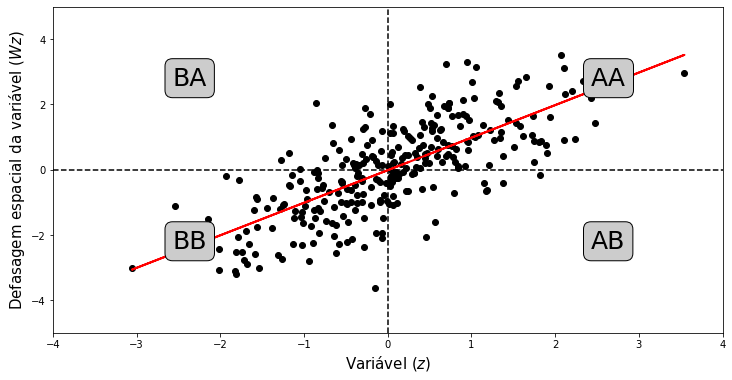
\includegraphics[width=0.7\textwidth]{figuras/moran_scatter.png}\\
	\parbox{\dimexpr\linewidth-5cm}{\raggedright
    \strut \textsuperscript{Fonte: Elaboração própria com dados simulados.}\strut}
\end{figure}

O diagrama de dispersão de Moran se divide em quatro quadrantes , como mostrado na Figura \ref{dispersaomoran_2}. No primeiro quadrante, o diagrama de Moran apresenta as observações do tipo Alto-Alto (AA), que representa as regiões que têm valor da variável em estudo acima da média, com regiões vizinhas que também possuem valores acima da média. Por sua vez, o segundo quadrante apresenta as observações do tipo Baixo-Alto (BA), que são as regiões com valores da variável analisada abaixo da média, rodeadas por regiões que possuem valores acima da média. Já o terceiro quadrante contém as observações chamadas de Baixo-Baixo (BB), que contempla regiões com valores abaixo da média, cujas regiões vizinhas também têm valores abaixo da média. Por fim, o quarto quadrante abrange as regiões do grupo  Alto-Baixo (AB), e compreende as regiões com valor alto, rodeadas por vizinhos de valores baixos para a variável.

\subsubsection{Autocorrelação espacial local}
	
Um indicador com a capacidade de detectar padrões locais de autocorrelação espacial é o $I_i$ de Moran local \cite{almeida12_g}. Este indicador foi proposto por Anselin em $1995$ e é uma estatística com capacidade de detectar padrões locais de autocorrelação espacial estatisticamente significativos. Ainda segundo Anselin (1995), um indicador que é capaz de identificar padrões locais de autocorrelação espacial é chamado \textit{``local indicator of spatial association} (LISA)". Esta classe de indicadores deve satisfazer dois critérios: 


\begin{enumerate}[leftmargin=1.8cm, label=\alph*)]
    \item o indicador deve ser capaz de indicar \textit{clusters} espaciais estatisticamente significativos para cada observação;
	\item o somatório dos indicadores locais, calculados para todas as regiões, deve equivaler ao indicador de autocorrelação espacial global para as mesmas regiões.
\end{enumerate}


Um exemplo de indicador do tipo LISA é o $I_i$ de Moran local. Este indicador decompõe o $I$ de Moran global em quatro categorias: Alto-Alto (AA), Baixo-Baixo (BB), Alto-Baixo (AB) e  Baixo-Alto (BA). Essas categorias são equivalentes aos quadrantes do diagrama de dispersão de Moran (Figura \ref{dispersaomoran_2}). O $I_i$ de Moran local para a variável padronizada $z_i$, observada na regão $i$, pode ser expressa como 
	
\begin{align*}
	I_i = z_i \sum_{j}^{} w_{ij} z_j.
\end{align*}

O cálculo de $I_i$ é realizado englobando apenas as regiões vizinhas de $i$, definidas por meio da matriz de pesos espaciais. Como o cálculo do $I_i$ é realizado para cada uma das $n$ observações, o que gera uma grande quantidade de informação, uma forma mais eficiente de visualizar o conjunto de estatísticas geradas é apresentá-las em um mapa de \textit{clusters}. Este mapa exibe uma combinação do diagrama de dispersão de Moran (Figura \ref{dispersaomoran_2}) com a significância do local $I_i$ \cite{almeida12_g}. 

	
%A Figura \ref{lisa_ex_2} apresenta um exemplo de um mapa de \textit{clusters} \textit{LISA}. A variável utilizada foi o número de apólices de seguro rural contratadas nos municípios do Brasil no ano de $2019$. O mapa da Figura \ref{lisa_ex_2} demonstra a classificação em quatro categorias de associação espacial estatisticamente significativas. 
	
%\begin{figure}[H]
%	\centering
%	\caption{Mapa de \textit{clusters LISA} para apólices contratadas de seguro rural no ano de 2019}
%	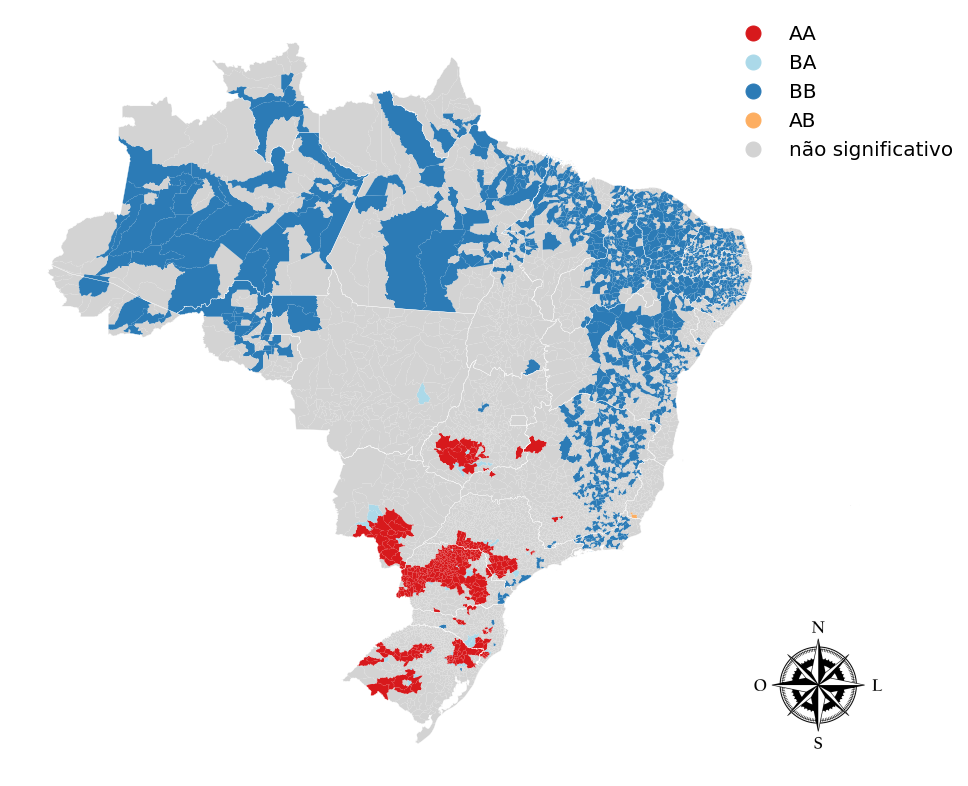
\includegraphics[width=0.6\textwidth]{figuras/map_lisa_ex.png}
%	\parbox{\dimexpr\linewidth-1.5cm}{\raggedright
%    \strut \textsuperscript{Fonte: Elaboração própria}\strut}
%    \label{lisa_ex_2}
%\end{figure}
	
%É necessário destacar que, ambas as estatísticas de autocorrelação espacial local, $G_i$ e $I_i$, apresentam vantagens e desvantagens. Com relação ao $G_i$, uma vantagem é a capacidade  de estabelecer uma definição mais clara de \textit{clusters} com valores altos  (\textit{hot spots}) ou \textit{clusters} com valores baixos (\textit{cool spots}). No entanto, este indicador traz a desvantagem de não ser capaz de indicar uma situação de associação espacial de valores dissimilares. Por sua vez, o $I_i$ é capaz de indicar autocorrelação negativa e possui a capacidade de revelar \textit{outliers} globais \cite{darmofal06_g}.


\subsection{ANÁLISE MULTIVARIADA}
	
Em uma pesquisa, os dados obtidos são considerados multivariados quando cada unidade amostral possui diversas variáveis aleatórias. A análise multivariada se caracteriza por um conjunto de métodos estatísticos que são utilizados para analisar as variáveis como um todo, levando-se em conta, por exemplo, a sua estrutura de correlação. Os métodos de análise multivariada possibilitam a realização de  uma avaliação muito mais ampla do conjunto de dados, permitindo encontrar padrões que, possivelmente, não seriam revelados ao se analisar cada variável separadamente \cite{mingoti10}. 
	
Segundo Hair \textit{et al.} (2009), os métodos multivariados podem ser divididos como métodos de dependência e interdependência. Se o estudo envolver variáveis com uma estrutura de dependência previamente identificada, aconselha-se que se faça uso de técnicas de dependência, tais como regressão múltipla, regressão logística ou análise discriminante. Entretanto, se não haver uma distinção preliminar entre quais variáveis são dependentes e independentes, aconselha-se que o uso de técnicas de interdependência, como análise fatorial e análise de agrupamento.
	
	
A representação de dados multivariados se dá através de matrizes. Uma amostra aleatória que contenha $n$ unidades amostrais ou observações, contendo valores de $p$ variáveis observadas, dá origem a uma matriz de dados $X$ com dimensão $n$ (linhas) por $p$ (colunas):
	
\begin{align}\label{X_2}
    X_{n \times p} =
	\left[
	\begin{array}{cccc}
	    X_{11} & X_{12} & \dots & X_{1p} \\
	    X_{21} & X_{22} & \dots & X_{2p} \\
	    \vdots & \vdots & \ddots & \vdots \\
	    X_{n1} & X_{n2} & \dots & X_{np}\\
	\end{array}
	\right],
\end{align}
	
\noindent em que cada unidade amostral é representada por uma linha da matriz de dados $X$, sendo um vetor com $p$ elementos (variáveis), e cada variável é representada por uma coluna de $X$, sendo um vetor com $n$ elementos \cite{everitt11}.
	
A representação de dados multivariados em uma matriz como apresentada na forma da definição (\ref{X_2}) pode não ser muito informativa, principalmente se o tamanho amostral $n$ for grande e houver um número abundante de variáveis $p$. Desse modo, torna-se relevante a utilização de medidas resumo dos dados amostrais, calculando-se a média, mediana, desvio padrão, por exemplo, de forma a sintetizar as informações dos dados da amostra \cite{ferreira11_g}.  
	
A média amostral, muito utilizada como uma medida de tendência central, torna-se o vetor de médias amostral no caso multivariado de dimensão $p \times 1$, onde cada elemento $\bar{X}_{i}$, com $i = 1,2,\cdots,p $, é a média de uma variável:
	
\begin{align*}
	\bar{X} = \left[
	\begin{array}{c}
    	\bar{X}_1\\
	    \bar{X}_2\\
	    \vdots\\
	    \bar{X}_p\\
    \end{array}
	\right].
\end{align*}
	
Como medida de dispersão dos dados, no caso multivariado, utiliza-se, no lugar da variância amostral, a matriz de covariâncias amostral $\boldsymbol{S}$ de dimensão $p \times p$. Em sua diagonal principal, estão as variâncias de cada uma das $p$ variáveis, enquanto os elementos fora da diagonal principal são as covariâncias entre as variáveis. A matriz de covariâncias amostral é simétrica, ou seja,  $S_{ij}$ $=$ $S_{ji}$.
	
	
\begin{align*}
	S =
	\left[
	\begin{array}{cccc}
    	S_{11} & S_{12} & \dots & S_{1p} \\
	    S_{21} & S_{22} & \dots & S_{2p} \\
	    \vdots & \vdots & \ddots & \vdots \\
	    S_{p1} & S_{p2} & \dots & S_{pp} 
	\end{array}
	\right].
\end{align*}        
	
A correlação também pode ser usada como uma medida de associação entre duas variáveis. Os valores do coeficiente de correlação variam entre $-1$ e $1$. Valores próximos de $1$ indicam que as variáveis estão fortemente correlacionadas de forma positiva, ou seja, grandes valores de uma estão associados a grandes valores da outra. Já valores próximos de $-1$ indicam que as variáveis estão fortemente correlacionadas de forma negativa, o que indica que grandes valores de uma estão associados a pequenos valores da outra. A matriz de correlações amostral é dada por 
	
\begin{align}
	R =
	\left[
	\begin{array}{cccc}
    	1      & r_{12} & \dots  & r_{1p} \\
	    r_{21} & 1 & \dots  & r_{2p} \\
	    \vdots & \vdots & \ddots & \vdots \\
	    r_{p1} & r_{p2} & \dots  & 1\\
	\end{array}
	\right].
	\label{def_matriz_corr_2}
\end{align}        
	
\noindent em que $r_{ij} = \frac{S_{ij}}{\sqrt{S_{ii} S_{jj}}}$ \cite{ferreira11_g}.  
	
\vspace{0.15cm} % só pra dar um espacinho :)
	
Outras estatísticas descritivas, como a matriz de somas de quadrados e produtos e a matriz de correlações, podem ser consideradas, dependendo do objetivo de estudo \cite{ferreira11_g}.
	
Assim como ocorre na análise univariada, as técnicas de estatística multivariada podem ser divididas em dois grupos, as técnicas exploratórias e as técnicas de inferência estatística. O primeiro grupo constitui-se de técnicas que não dependem do conhecimento da forma matemática da distribuição de probabilidade que gerou os dados amostrais. Além disso, o uso dessas técnicas permite a identificação de padrões em dados multivariados, fazendo com que possuam grande apelo prático. São exemplos de técnicas exploratórias: análise de componentes principais, análise fatorial exploratória e análise de agrupamento. Por outro lado, o grupo de técnicas de inferência estatística tem como objetivo a estimação de parâmetros, testes de hipóteses, análise de regressão multivariada etc.  Portanto, as técnicas de inferência fazem uso da amostra para realizar inferências sobre a população de onde essa amostra foi extraída \cite{mingoti10}.
	
\subsubsection{Análise de componentes principais} \label{ACP} 
	
A análise de componentes principais (ACP) tem como objetivo, explicar a estrutura de covariâncias das $p$ variáveis, $X^T = [X_1 \quad X_2 \quad \dots \quad X_p]$, por meio de combinações lineares das variáveis originais. Os componentes principais são as $p$ combinações lineares obtidas, $Y^T = [Y_1 \quad Y_2 \quad \dots \quad Y_p]$, e não sendo correlacionados entre si. Os componentes principais são ordenados de forma que suas primeiras combinações lineares já contabilizem a maior parte da variância presente em todas as variáveis originais, consequentemente, podendo ser usados para fornecer uma redução das dimensões dos dados \cite{mingoti10, everitt11}.
	
Vários critérios podem ser adotados para selecionar o número de componentes, de forma que grande parte da variância total seja explicada por um pequeno conjunto das novas variáveis. Com  uma grande quantidade de variação das variáveis originais explicada pelos $(k)$ primeiros componentes principais, ocorre uma simplificação da estrutura de covariâncias das variáveis originais. A ACP pode ser utilizada como uma ferramenta para auxiliar em outras técnicas, como ocorre em problemas de multicolinearidade na regressão linear, por exemplo \cite{ferreira11_g}.
	
O primeiro componente principal $Y_1$ é a combinação linear
\begin{align*}
	Y_1 = a_{11}X_1 + a_{12}X_2 + \dots + a_{1p}X_p,
\end{align*}
cuja variância amostral é a maior dentre todas as outras combinações lineares. O vetor de coeficientes referente ao $j$-ésimo CP é representado por $\boldsymbol{a}_j= [a_{j1} \quad a_{j2} \quad \dots \quad a_{jp}]$. É importante usar uma restrição nos valores desses coeficientes, como $\boldsymbol{a}_1^T\boldsymbol{a}_1 = 1$, ou seja, a soma dos quadrados desses valores deve ser igual a $1$. Isso deve ser feito porque a variância de $Y_1$ poderia crescer de forma ilimitada apenas aumentando os coeficientes $\boldsymbol{a}_1$. A variância amostral de $Y_1$ é dada por $\boldsymbol{a}_1^T S\boldsymbol{a}_1$, sendo $\boldsymbol{S}$ a matriz de covariâncias amostral das $X$ variáveis e $\boldsymbol{a}_1$ é o autovetor da matriz $S$ associado ao maior autovalor $\lambda$ dessa matriz \cite{everitt11}. A obtenção de autovalores $\lambda$ e autovetores $\boldsymbol{e}$ de uma matriz quadrada $p \times p$ são tais que $\boldsymbol{A}\boldsymbol{e} = \lambda\boldsymbol{e}$. Para maiores detalhes, consultar Ferreira (2011).
	
Ainda de acordo com os autores, o segundo componente principal, $Y_2$, definido como a combinação linear
\begin{align*}
	Y_2 = a_{21}X_1 + a_{22}X_2 + \dots + a_{2p}X_p,
\end{align*}
ou seja, $Y_2 = \boldsymbol{a}_2^T\boldsymbol{X}$, em que $\boldsymbol{a}_2^T = [a_{21} \quad a_{22} \quad \dots \quad a_{2p}]$ e $\boldsymbol{X}^T = [X_{1} \quad X_{2} \quad \dots \quad X_{p}]$, que possui a maior variância sujeito às condições
\begin{align*}
	\boldsymbol{a}_2^T\boldsymbol{a}_2 = 1,\\
	\boldsymbol{a}_2^T\boldsymbol{a}_1 = 0,
\end{align*}
em que a segunda condição garante que $Y_1$ e $Y_2$ são não correlacionados. Todos os componentes são obtidos de forma similar.
	
O vetor de coeficientes que define o $j$-ésimo componente principal, $\boldsymbol{a}_j$, é o autovetor de $\boldsymbol{S}$ associado com o seu $j$-ésimo maior autovalor. A variância do $j$-ésimo componente principal é dada por $\lambda_j$, sendo  $\lambda_1, \lambda_2, \dots, \lambda_p$ os autovalores de $\boldsymbol{S}$ sujeitos à restrição $\boldsymbol{a}_j^T\boldsymbol{a}_j = 1$ \cite{everitt11}.
	
A proporção da variância total de $\boldsymbol{X}$ explicada pelo $j$-ésimo componente principal é definida por
\begin{align*}
	\dfrac{Var(Y_j)}{\textrm{Variância total de } X} = \dfrac{\lambda_j}{\textrm{traço}(\boldsymbol{S})} = \dfrac{\lambda_j}{\displaystyle\sum_{i=1}^{p}\lambda_i}.
\end{align*}
	
%Além disso, as variâncias total e generalizada de $\boldsymbol{X}$ podem ser descritas pelas variâncias total e generalizada de $\boldsymbol{Y}$:
%\begin{align*}
%	\textrm{traço}(\boldsymbol{S}) = \displaystyle\sum_{i=1}^{p}\lambda_i = S_1^2 + S_2^2 + \dots + S_p^2 \quad \textrm{ e} \quad |\boldsymbol{S}| = \prod_{i=1}^{p}\lambda_i.
%\end{align*}
	
%Dessa forma, os vetores $\boldsymbol{X}$ e $\boldsymbol{Y}$ são equivalentes em relação a essas duas medidas de variação. Além disso, sempre o primeiro componente principal tem a maior proporção de explicação da variância total de $\boldsymbol{X}$ \cite{mingoti10}.
	
De acordo com Everitt e Hothorn (2011), os primeiros $k$ componentes, em que $k < p$, explicam uma proporção da variância total,
	
\begin{align*}
    \dfrac{\displaystyle\sum_{j=1}^{k}Var(Y_j)}{\textrm{Variância total de } X} = \dfrac{\displaystyle\sum_{j=1}^{k}\lambda_j}{\textrm{traço}(\boldsymbol{S})} = \dfrac{\displaystyle\sum_{j=1}^{k}\lambda_j}{\displaystyle\sum_{j=1}^{p}\lambda_j}.
\end{align*}
	
Os componentes principais podem ser obtidos a partir da matriz de covariâncias amostrais $S$ ou a partir da matriz de correlações amostrais $R$. A extração dos componentes da matriz de covariâncias deve ser preferido quando as variáveis originais estão na mesma escala, o que é raro ocorrer. Extrair os componentes, como os autovetores de $R$ é equivalente a calcular os componentes das variáveis originais para, em seguida, padronizar cada um para ter variância igual a $1$ \cite{everitt11}.
	
Ainda segundo Everitt e Hothorn (2011), os componentes principais são variáveis aleatórias que podem ser observadas apenas a partir da observação de um vetor aleatório $\boldsymbol{X}$. Os escores dos CPs são obtidos pela substituição dos valores observados de $\boldsymbol{X}$ em cada um dos componentes $Y_j$. Se os CPs forem obtidos a partir da matriz de covariâncias $S$, os escores $Y^*_{ji}$ dos $k$ componentes para cada observação $i$ são dados por:  
	
\begin{align*}
	Y^*_{1i} & =\boldsymbol{a}_1^T\boldsymbol{X}_i\\
	Y^*_{2i} & =\boldsymbol{a}_2^T\boldsymbol{X}_i\\
	&\vdots\\
	Y^*_{ki} & =\boldsymbol{a}_k^T\boldsymbol{X}_i.
\end{align*}
	
Estes são geralmente utilizados na condução de análises estatísticas de dados ou simplesmente para ordenação, identificando aquelas observações que possuem os maiores ou menores valores globais dos componentes \cite{mingoti10}.


%=========================================================================================================
%111111111111111111111111111111111111111111111111111111111111111111111111111111111111111111111111111111111
% Capítulo 1

\newpage
\pagenumbering{arabic}
\pagestyle{fancy}

\setlength{\parindent}{1.25cm}
\setlength{\parskip}{0ex}

%% reinicia contadores de página e demais ambientes
\setcounter{page}{32}
\setcounter{section}{0}
\setcounter{figure}{0}
\setcounter{table}{0}
\setcounter{equation}{0}

%% definições de título
\def\titlecapa{O seguro rural no Brasil: evolução e distribuição regional}
\def\titlecapA{\expandafter\MakeUppercase\expandafter{\titlecapa}}
\addcontentsline{toc}{section}{\hspace*{\distnumber}ARTIGO 1 -- \titlecapa}

%%.....................................................
%% inclui título
\begin{center}
\noindent
%\begin{minipage}[t]{0.2\textwidth}
\textbf{ARTIGO 1 - }
%\end{minipage}
%\begin{minipage}[t]{0.8\textwidth}
%\begin{flushleft}
\textbf{\titlecapA} 
%\end{flushleft}
%\end{minipage}
\end{center}
\vspace{0.8cm}

%%.....................................................
%% inclui resumo e abstract

%\begin{center}
\noindent\textbf{RESUMO} 
\vspace{0.8cm}
%\end{center}
%\vspace{1cm}
\begin{singlespace}
\noindentAs atividades agropecuárias se inserem em um contexto de adversidades que as colocam em situação diferenciada em relação aos riscos enfrentados pelos produtores. Tais atividades demandam grandes investimentos, o que faz com que sua atratividade esteja relacionada às formas existentes de gerenciamento de riscos. Uma das formas mais usuais de gerenciamento de risco neste setor é a contratação de Seguro Rural, uma vez que esta modalidade de seguro possibilita a recuperação da capacidade financeira do produtor na ocorrência de sinistros. Nesse sentido, o objetivo do trabalho é avaliar a distribuição e a dinâmica espacial de variáveis relacionadas às apólices de Seguro Rural contratadas nos municípios brasileiros no período de 2006 a 2019. Além disso, busca-se investigar a existência de dependência espacial e a presença de agrupamentos com grande número de apólices de Seguro Rural. Para tanto, utiliza-se os dados dos Censos do Seguro Rural, compilados pelo Ministério da Agricultura, Pecuária e Abastecimento (MAPA) e Análise Exploratória de Dados Espaciais (AEDE). Os resultados apontam que as maiores concentrações de apólices de Seguro Rural estão situadas nas regiões Sul e Centro-Oeste. Além disso, apesar de haver um aumento nas contratações de Seguro Rural, há também uma tendência de maior concentração espacial das apólices ao longo do período analisado. \\
\newline
\noindent {\textbf{Palavras-chave}}: Seguro rural. Política agrícola. Estatística espacial. Autocorrelação espacial. I de Moran.
\end{singlespace}

\vspace{1cm}
%\begin{center}
\noindent\textbf{ABSTRACT}
\vspace{0.8cm}
%\end{center}
\begin{singlespace}
\noindent   \noindent Agricultural activities demand large investments. Therefore, the context of adversities, in which these activities are inserted, presents a risk scenario that encourages producers to search for existing forms of risk management. One of the most common forms of risk management in this sector is the contracting of Rural Insurance, since this type of insurance makes it possible to recover the financial capacity of the producer in the event of claims. In this sense, the objective of this work is to evaluate the evolution and the spatial dynamics of variables related to Rural Insurance policies contracted in Brazilian municipalities from 2006 to 2019. For this, data were taken from the Rural Insurance Census, compiled by the Ministry of Agriculture, Livestock and Supply. The results indicate that the highest concentrations of Rural Insurance policies are located in the South, Southeast and Midwest regions. In addition, despite an increase in Rural Insurance contracts, there is also a trend of greater spatial concentration of policies over the analyzed period. \\ 
\newline
\noindent {\textbf{Keywords}}:  Rural insurance. Agricultural policy. Agricultural risk management. Subvention.

\end{singlespace}

%%.....................................................
%% inclui capítulo

\newpage
\section{INTRODUÇÃO}

O setor agropecuário brasileiro tem se destacado nas últimas décadas por seu crescimento proveniente da aplicação de novas tecnologias ao clima tropical e a incorporação de novas áreas de terras \cite{brasil19a}. Segundo dados dos censos agropecuários, entre $2006$ e $2017$, tanto a área total quanto a produção agrícola e pecuária vivenciaram crescimento. Neste período houve um acréscimo de cerca de $5,8\%$ na área total dos estabelecimentos agropecuários \cite{ibge19}. Com relação à sua participação no PIB, em 2019, a parcela do agronegócio brasileiro foi de  $20,5\%$  do PIB nacional. Já em 2020, o setor agropecuário brasileiro alcançou a participação de $26,6\%$ do PIB. Em valores monetários, o PIB do País totalizou R\$ $7,45$ trilhões em 2020, e a participação do agronegócio chegou a quase R\$ $2$ trilhões \cite{cepea21}. 

Dada a relevância do setor agropecuário na economia brasileira, é necessário destacar que este ramo apresenta características muito específicas com relação à magnitude dos riscos aos quais está sujeito \cite{burgo05}. Alguns riscos mais relevantes se devem, principalmente, às instabilidades climáticas e ameaças sanitárias, que podem afetar a produção, ou à razões de mercado, como variações das taxas de câmbio e juros, ou a condições ligadas ao ambiente de negócios, tais como, alterações em marcos regulatórios e em políticas públicas. Todos esses fatores geram variações na renda do setor, que devem ser enfrentadas por meio de políticas de apoio à gestão de riscos \cite{brasil21}. 

Uma gestão de riscos apropriada tem potencial de afetar de forma positiva a estabilidade da renda do produtor e sua própria permanência no setor agropecuário. O gerenciamento de riscos agropecuários pode ocorrer de diversas maneiras, no entanto, a contratação de seguro é uma das medidas mais comuns. O seguro rural é uma importante ferramenta de mitigação de riscos e proteção da renda. Esta modalidade de seguro atua no sentido de amenizar as perdas e possibilitar a recuperação da capacidade financeira do produtor rural em caso de ocorrência de sinistros \cite{brasil19b}. 

Nesse sentido, o presente trabalho tem por objetivo, avaliar a distribuição espacial do seguro rural nos municípios brasileiros entre 2006 e 2019. Para tanto, busca-se investigar se, no Brasil, as variáveis de seguro rural se distribuem de forma aleatória no espaço ou se há padrões de distribuição espacial. Além disso, através da análise da distribuição espacial do seguro rural no período, busca-se identificar se há regiões que tiveram alterações significativas no número de contratações de seguro. Por fim, este estudo busca fornecer informações para o debate de aperfeiçoamentos no sistema de seguro rural brasileiro, de forma a contribuir para uma agricultura mais eficiente e com menores riscos para o produtor rural.

O trabalho está estruturado da seguinte forma: a próxima seção apresenta uma breve revisão de literatura sobre o seguro rural. A terceira seção apresenta os dados, os procedimentos de análise e recursos computacionais que serão utilizados. A quarta seção apresenta resultados e discussões. A última seção apresenta as considerações finais.

\section{UM PANORAMA DO SEGURO RURAL NO BRASIL}

No Brasil, as primeiras iniciativas de se instalar um sistema de seguro rural remontam à meados da década de $1930$ e desenvolveram-se principalmente nas esferas estaduais. Em $1939$, o Estado de São Paulo determinou a criação de um seguro obrigatório contra o granizo na produção de algodão \cite{maia11}. Segundo Silva, Teixeira e Santos (2014), os resultados do seguro para a proteção da lavoura algodoeira em São Paulo influenciaram a criação de novos programas como a Carteira de Seguro Agrícola contra Granizo para a Viticultura, criada em $1948$, e a Carteira de Seguro Agrícola contra Geada para Horticultura instituída em $1964$.

Além disso, Silva, Teixeira e Santos (2014) apontam em seu trabalho o seguro para granizo que foi criado no final da década de $1940$ no Instituto Rio-Grandense do Arroz (Irga), e o seguro criado pela Associação dos Fumicultores do Brasil (Afubra), que objetivava ressarcir com recursos próprios os produtores de fumo nos estados de Santa Catarina e Rio Grande do Sul.

Já no âmbito nacional, foi criado em $1948$, o Instituto de  Resseguros do Brasil (IRB), com o objetivo de reduzir os prejuízos de eventos adversos e assegurar uma maior estabilidade aos produtores rurais \cite{silva14}. Além disso, o Governo Federal criou, em $1954$, a Companhia Nacional de Seguro Agrícola (CNSA) e o Fundo de Estabilidade do Seguro Agrário. Para mais, Maia,  Roitman e de Conti (2011) evidenciaram que a estruturação e gestão dos seguros da CNSA ficaram, de início, sob responsabilidade do IRB. No entanto, segundo Gemignani (2000), as atividades da CNSA se encerraram em $1996$, em decorrência do insucesso em disseminar a adesão ao seguro rural de forma a possibilitar sua viabilidade econômica \cite{maia11, silva14}.

Na segunda metade da década de $1960$, são instituídos o Decreto-Lei nº $73$ ($1966$) e o Decreto nº $60.459$ ($1967$), que instituem os fundamentos institucionais para as atividades de seguro e a criação do Sistema Nacional de Seguros Privados (SNSP). O decreto de $1967$ também criou o Fundo de Estabilidade do Seguro Rural (FESR), cujos recursos inicialmente eram geridos pelo IRB e cujo objetivo principal era garantir a equilíbrio do sistema de seguro rural e fornecer uma cobertura adicional para os riscos de sinistro \cite{silva14}

% Até aqui Ok
Instituída em $1970$, a Resolução nº $5$ do Conselho Nacional de Seguros Privados teve uma função relevante na caracterização das modalidades de seguros agrários. Nesta Resolução, foi definido o seguro agrícola, que fornece cobertura contra perdas decorrentes de fenômenos meteorológicos, doenças e pragas, o seguro pecuário que fornece cobertura para morte de animais causadas por doenças ou acidentes, assim como, o seguro de benfeitorias e produtos agropecuários. Em suma, a Resolução nº $5$ também estabelece o seguro de crédito, que cobre incapacidade de pagamento de compradores dos produtos agropecuários \cite{silva14}.

A criação do Programa de Garantia da Atividade Agropecuária (Proagro), através da Lei nº $5.969$, de $11$ de dezembro de $1973$ ocorreu devido ao fato de que, apesar das diversas ações do Governo Federal, o seguro rural se desenvolveu de forma lenta e restrita à uma pequena parcela da produção \cite{silva14}. O Proagro inicialmente ficou sob a responsabilidade do Banco Central e passou a vincular o seguro rural às operações de crédito agropecuário. Por sua vez, o Banco Central utilizou emissões monetárias para pagamentos de sinistros. Segundo Maia, Roitman e De Conti (2011), o sistema de financiamento do Proagro gerou déficits que provocaram diversas alterações no Programa, que ainda permanece um dos mais importantes instrumentos para a gestão de riscos na agricultura no Brasil.

Instituído por meio da Lei nº $10.823$ de $19$ de dezembro de $2003$ e do Decreto nº $5.121$ de $2004$, o Programa de Subvenção ao Prêmio do Seguro Rural (PSR), passou a ser a política adotada pelo Governo Federal para o estímulo ao sistema de seguro rural no Brasil \cite{brasil18}. O PSR busca, assim como ocorre em países europeus e nos Estados Unidos, conceder subvenção econômica ao valor do prêmio do seguro rural contratado com seguradoras autorizadas \cite{maia11, silva14}.

Dessa forma, o PSR tem como finalidade subsidiar parte do prêmio do seguro rural, de modo a assegurar a responsabilidade do seguro rural como forma de garantir a estabilidade da renda do produtor, além de suscitar o aplicação das tecnologias adequadas para os empreendimentos agropecuários \cite{guia_20}. Tal política do governo busca tornar o seguro rural mais acessível aos agricultores, dividindo os custos de aquisição da apólice entre o governo e os produtores. 


\section{MATERIAL E MÉTODOS}\label{material_e_metodos}

%O objetivo dessa seção é apresentar os dados utilizados no trabalho, descrever a metodologia e os recursos computacionais utilizados na presente análise.

\subsection{DADOS}

% Fonte dos Dados 

Os dados de seguro rural utilizados neste trabalho foram obtidos no endereço eletrônico do Ministério da Agricultura, Pecuária e Abastecimento (MAPA) \cite{brasil21}. Foram utilizados dados com valores anuais a partir do ano de $2006$ até o ano de $2019$ (último ano disponível até então) para os dados municipais. Os dados agregados são provenientes do Atlas do Seguro Rural do MAPA e apresentam periodicidade anual a partir do ano de $2006$. Também foram utilizados dados que contém atributos geográficos, como a posição e o formato, do território brasileiro. Esses dados estão disponíveis no endereço eletrônico do Instituto Brasileiro de Geografia e Estatística \cite{ibge20}.

O conjunto de dados de seguro rural possui informação referente à localização geográfica da contratação do seguro rural. No entanto, foram detectadas algumas divergências relacionadas a distritos ou outras localidades, como fazendas e vilarejos, que foram apontados como o local referente à contratação do seguro. 

Para corrigir essas divergências, de forma a ter informações referentes apenas aos municípios brasileiros, as informações relacionadas às demais localidades foram acrescentadas aos municípios correspondentes. Para a identificação, foi feita uma busca de cada localidade que não tinha correspondência com os municípios brasileiros. Essa busca foi feita inicialmente no site \textit{google maps}, contendo, como termo de busca, o nome da localidade e o seu estado \footnote{Foi considerado que a informação referente aos Estados estava correta nos dados do MAPA}. Nos casos em que a informação do município ao qual a localidade pertencia estava disponível no resultado da pesquisa, o nome do município era utilizado em uma segunda busca no site \textit{Portal Cidades} do IBGE \footnote{\url{https://cidades.ibge.gov.br}}. O \textit{Portal Cidades} apresenta, na maioria dos casos, a divisão territorial e administrativa atualizada, de forma a possibilitar a correção das divergências nos dados. Nos casos em que a informação do município ao qual a localidade pertencia não estava disponível no resultado da pesquisa, o nome da localidade era utilizado como termo de busca de CEPs no site dos Correios \footnote{\url{https://buscacepinter.correios.com.br/app/localidade_logradouro/index.php}}. Para os casos em que não foi possível encontrar nenhum resultado com relação ao município correspondente, a localidade em divergência foi atribuída ao município geograficamente mais próximo \footnote{Os códigos utilizados na análise estão disponíveis no \textit{GitHub} e os link estão no Apêndice B.}.

% Editar essa parte!!!!!
%Variáveis total de apólices contratadas (TAC), soma da importância segurada (R\$ milhão) (SIS), soma dos prêmios (R\$ milhão) (SPR), total de subvenção (R\$ milhão) (TSB), soma das indenizações pagas (R\$ milhão) (SIP), taxa média aplicada às apólices (TMA) e número de apólices indenizadas (NAI).

%\subsection{ANÁLISE DOS DADOS} 

%Após uma análise exploratória dos dados, foi realizada a primeira parte da Análise Exploratória de Dados Espaciais (AEDE), onde os dados agregados por municípios serão apresentados por meio de mapas temáticos, de forma a ilustrar o padrão espacial das variáveis de seguro rural. No segundo passo da AEDE, o valor do \textit{I} de Moram global foi calculado e sua significância obtida por meio do pseudo valor-$p$, obtido a partir de $999$ permutações aleatórias. Neste estudo, foi considerado um nível de significância $\alpha = 0,05$. Foi adotada a matriz de pesos espaciais de contiguidade com a convenção rainha, considerando os vizinhos de primeira ordem. Tal matriz foi adotada por ser a mais utilizada na literatura em trabalhos semelhantes \cite{almeida12}. 

%Para a construção da matriz de pesos espaciais, foram retirados os municípios de Fernando de Noronha, que se constitui em um arquipélago pertencente ao estado de Pernambuco, e Ilhabela, arquipélago no litoral norte do estado de São Paulo. Estes municípios foram desconsiderados pois, além de se constituírem de ilhas, não possuem nenhuma apólice de seguro rural contratada durante os anos em análise. Uma vez definida a matriz, se o valor do \textit{I} de Moran global for significativo, a hipótese de aleatoriedade espacial deve ser rejeitada e há evidências de que há uma autocorrelação positiva \cite{almeida12}. 

%O terceiro passo da análise espacial das variáveis de seguro rural consistiu na obtenção dos mapas \textit{LISA}, de forma a identificar padrões locais de autocorrelação espacial e \textit{outliers} espaciais. Esses mapas ilustram cada uma das observações e indicam se seus valores foram considerados significativos em relação à estatística do I de Moran local \cite{almeida12, anselin95}. 

%\subsection{RECURSOS COMPUTACIONAIS}  

Esse estudo foi feito utilizando a linguagem de programação \textit{Python} \cite{python17}, através da interface \textit{Jupyter} \cite{jupyter17} \cite{perez07} \cite{kluyver19}; Além disso, foram utilizadas as seguintes bibliotecas: \textit{Pandas} \cite{mckinney10}, que é uma ferramenta  para análise e manipulação de dados; \textit{NumPy} \cite{walt11}, que é destinado a possibilitar a computação numérica com \textit{Python}; \textit{SciPy} (JONES et al., 2001); % rever essa citação 
\textit{Matplotlib} \cite{hunter07} e \textit{Seaborn} \cite{waskom14}, que são bibliotecas para criar visualizações  de dados em \textit{Python}; \textit{jenkspy}, para a utilização do algoritmo Fisher Jenks \cite{jenks77} e \textit{Geopandas} \cite{jordahl14}, que possibilita a construção dos mapas. 

\section{RESULTADOS E DISCUSSÃO}

\subsection{A EVOLUÇÃO DO SEGURO RURAL} 

Inicialmente, serão apresentados dados ilustrativos da trajetória do Seguro Rural no Brasil. Serão analisados dados anuais referentes ao número de apólices contratadas, ao número de apólices indenizadas, aos valores de subvenção, indenização e prêmio. Também serão apresentados dados referentes à participação das seguradoras e das principais culturas no número de apólices contratadas. Foram utilizados dados da Plataforma Atlas do Seguro Rural. É importante destacar que os valores referentes ao ano de $2021$ ainda não estavam consolidados na data do presente estudo.

%\subsubsection{Apólices contratadas}

Nesta seção, serão analisados dados anuais referentes às apólices de seguro rural contratadas e os respectivos valores de prêmio e subvenção. 

No gráfico da Figura \ref{apolices_produtores}, é possível observar a evolução do número de produtores e do número de apólices de seguro rural contratadas no período de $2006$ a $2020$. Durante o período analisado, cada produtor contratou, em média, $1,48$ apólices de seguro rural. O número de apólices contratadas tem um crescimento de cerca de $8,69$ vezes durante o período. Entre os anos $2014$ e $2015$, ocorre uma queda de $66,08\%$ nas apólices contratadas. Por sua vez, o número de produtores cresceu $6,36$ vezes entre $2006$ e $2020$.

\begin{figure}[H]
	\centering
	\caption{Número de produtores e apólices de seguro rural contratadas. Brasil $2006 - 2020$}
	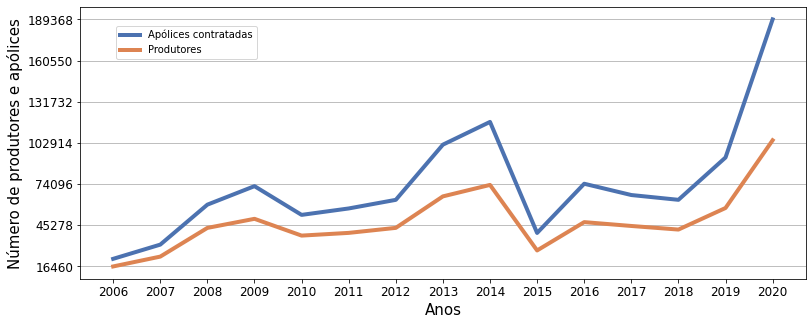
\includegraphics[width=0.8\textwidth]{figuras/apolices_produtores.png}\\
	%\small \textsuperscript {Fonte: Elaboração própria a partir de dados da Plataforma Atlas do Seguro Rural \cite{brasil21b}.}
    \parbox{\dimexpr\linewidth-3cm}{\raggedright
    \strut \textsuperscript{Fonte: Elaboração própria a partir de dados da Plataforma Atlas do Seguro Rural \cite{brasil21b}.}\strut}
    \label{apolices_produtores}
\end{figure}

É importante destacar que, no ano de $2021$, até o mês de junho, havia $66.928$ apólices contratadas \cite{brasil21}. Apesar do valor ser baixo se comparado ao ano de $2020$ ($189.368$ apólices), já é superior a $56,25\%$ dos anos anteriores. Padrão semelhante se observa com o número de produtores. No ano de $2021$, até o mês de junho haviam sido contabilizados $47.472$ produtores segurados \cite{brasil21b}.

%\subsubsection{Valores do prêmio e de subvenção ao prêmio de seguro rural}

O gráfico da Figura \ref{soma_ano_values} apresenta a evolução dos valores em milhões de reais de subvenção ao prêmio de seguro rural, prêmio pago pelo produtor e prêmio recebido pela seguradora entre $2006$ a $2020$. Observa-se que, com exceção do ano de $2014$, é possível notar uma tendência de crescimento dos valores de subvenção e prêmio pagos no período analisado. No ano de 2014, devido à contenções, o governo federal liberou apenas R\$ $400$ milhões dos R\$ $700$ milhões previstos para subsidiar o seguro rural. Esta contenção dos gastos governamentais pode ser um fator a ser considerado na queda dos valores do seguro rural ocorrida entre os anos de $2014$ e $2015$ \cite{andrade21}.

Em $2021$, até o mês de junho, o valor do prêmio pago à seguradora já havia alcançado R\$$1,25$ bilhões, o quarto maior valor registrado e cerca de $50,59\%$ maior que a média. O prêmio do produtor referente ao período de janeiro a junho de $2021$ já era equivalente a R$\$0,77$ bilhões, valor cerca de $69,67\%$ maior que a média do prêmio de responsabilidade do produtor. O valor concedido na forma de subvenção ao prêmio em $2021$ também é o quarto maior valor registrado, cerca de $25,96\%$ maior que a média dos valores de subvenção concedidos . Além disso, a partir do ano de $2016$, a parcela do prêmio sob responsabilidade do produtor passa a superar a parcela concedida pelo governo na forma de subvenção \cite{brasil21b}.

%\begin{figure}[H]
%	\centering
%	\caption{Valores do prêmio e de subvenção ao prêmio de seguro rural. Brasil $2006 - 2020$}
%	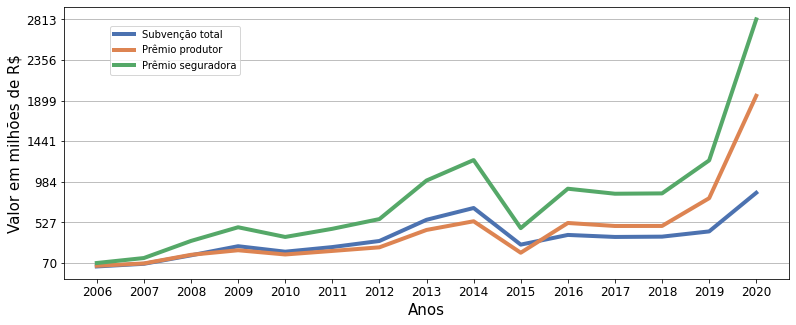
\includegraphics[width=0.8\textwidth]{figuras/soma_ano_values.png}\\
%	\small \textsuperscript {Fonte: Elaboração própria a partir de dados da Plataforma Atlas do Seguro Rural (Mapa, 2021).}
%    \label{soma_ano_values}
%\end{figure}

%\begin{figure}[H]
%	\centering
%	\caption{Soma da importância segurada (R\$ milhões). Brasil $2006 - 2020$}
%	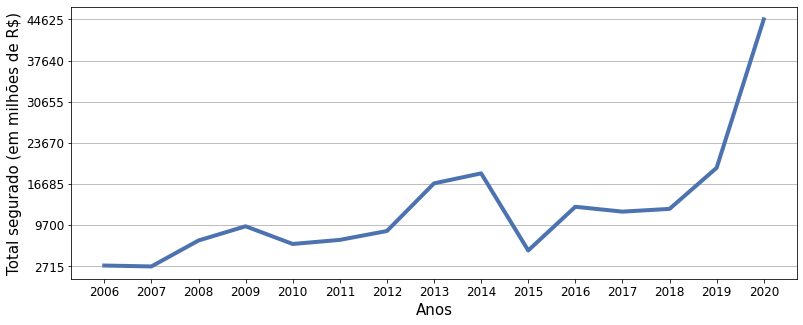
\includegraphics[width=0.8\textwidth]{figuras/total_segurado_mil.png}\\
%	\small \textsuperscript {Fonte: Elaboração própria a partir de dados da Plataforma Atlas do Seguro Rural (Mapa, 2021).}
%    \label{total_segurado_mil}
%\end{figure}

%\begin{figure}[H]
%	\centering
%	\caption{Total da área segurada em hectares. Brasil $2006 - 2020$}
%	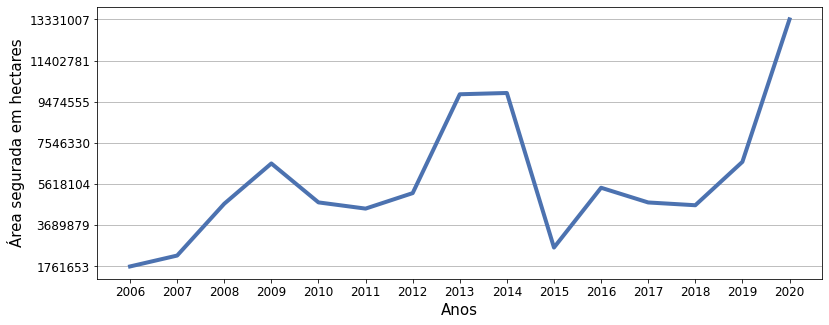
\includegraphics[width=0.8\textwidth]{figuras/area_segurada.png}\\
%	\small \textsuperscript {Fonte: Elaboração própria a partir de dados do Ministério da Agricultura, Pecuária e Abastecimento (MAPA).}
%    \label{area_segurada}
%\end{figure}

%\begin{figure}[H]
%	\centering
%	\caption{Número de apólices de seguro rural indenizadas. Brasil $2006 - 2019$}
%	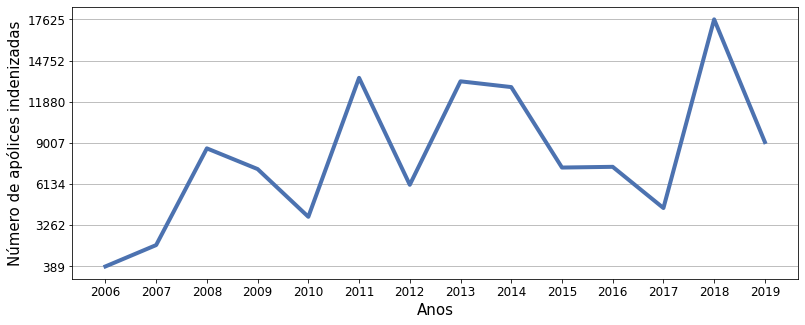
\includegraphics[width=0.8\textwidth]{figuras/apolices_indenizadas.png}\\
%	\small \textsuperscript {Fonte: Elaboração própria a partir de dados do Ministério da Agricultura, Pecuária e Abastecimento (MAPA)}
%    \label{apolices_indenizadas}
%\end{figure}

%\begin{figure}[H]
%	\centering
%	\caption{Valor das indenizações de seguro rural pagas (R\$ milhões). Brasil $2006 - 2019$}
%	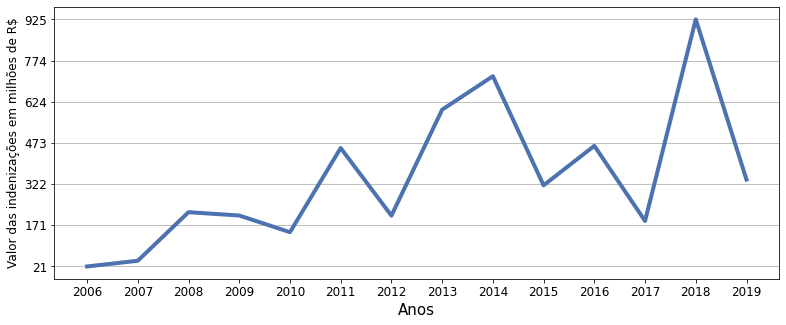
\includegraphics[width=0.8\textwidth]{figuras/valor_indenizacoes.png}\\
%	\small \textsuperscript {Fonte: Elaboração própria a partir de dados do Ministério da Agricultura, Pecuária e Abastecimento (MAPA)}
%    \label{valor_indenizacoes}
%\end{figure}

% variaveis_br
\begin{figure}[H]
	\centering
	\caption{Evolução das variáveis de seguro rural no Brasil}\label{variaveis_br}
	\small
	
	\subfloat[Valores do prêmio e de subvenção ao prêmio de seguro rural\label{soma_ano_values}]{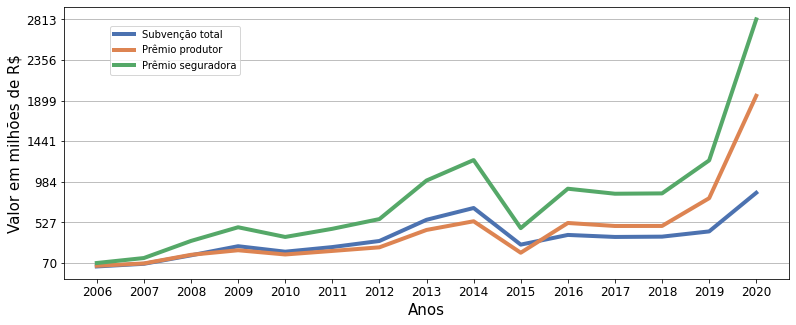
\includegraphics[width=0.45\textwidth]{figuras/soma_ano_values.png}}\hspace{0.1cm}
	\subfloat[Soma da importância segurada (R\$ milhões)\label{total_segurado_mil}]{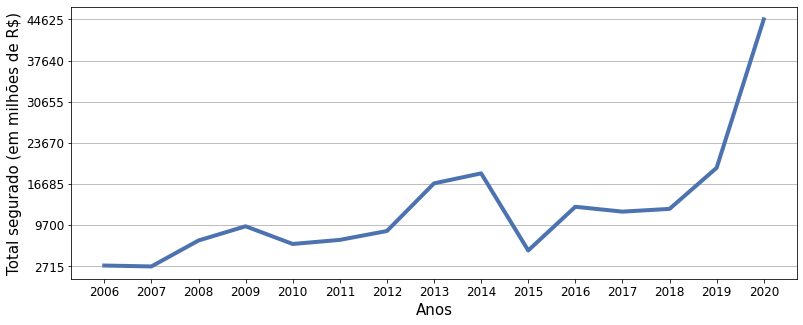
\includegraphics[width=0.45\textwidth]{figuras/total_segurado_mil.png}}\hspace{0.1cm}\\
	
	\subfloat[Total da área segurada em hectares.\label{area_segurada}]{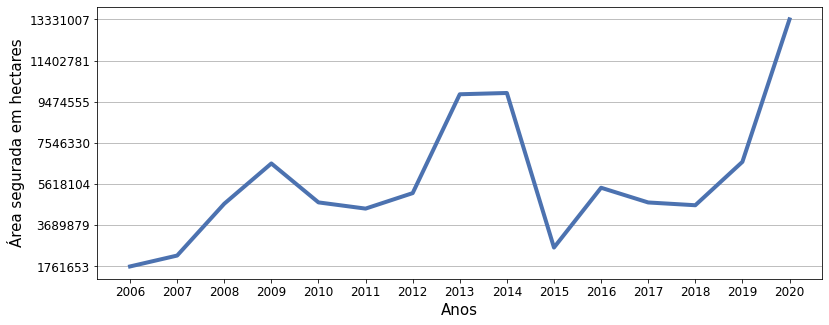
\includegraphics[width=0.45\textwidth]{figuras/area_segurada.png}}\hspace{0.1cm}
	\subfloat[Número de apólices de seguro rural indenizadas\label{apolices_indenizadas}]{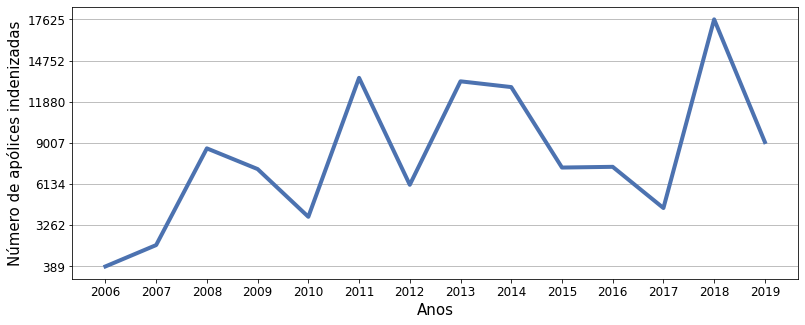
\includegraphics[width=0.45\textwidth]{figuras/apolices_indenizadas.png}}\\
	
	\subfloat[Valor das indenizações de seguro rural pagas (R\$ milhões)\label{valor_indenizacoes}]{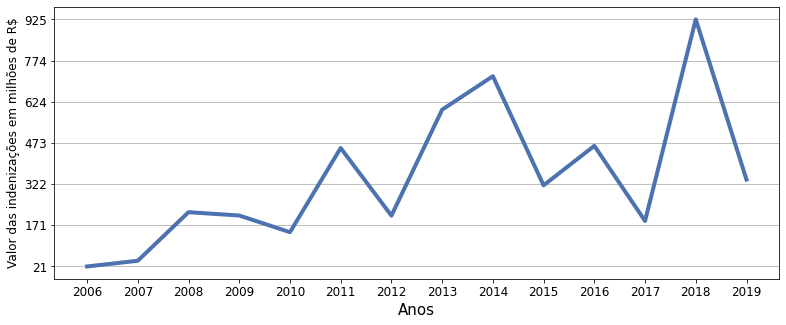
\includegraphics[width=0.45\textwidth]{figuras/valor_indenizacoes.png}}\hspace{0.1cm}
	\subfloat[Taxa média anual de contratação do prêmio de seguro rural\label{taxa_media}]{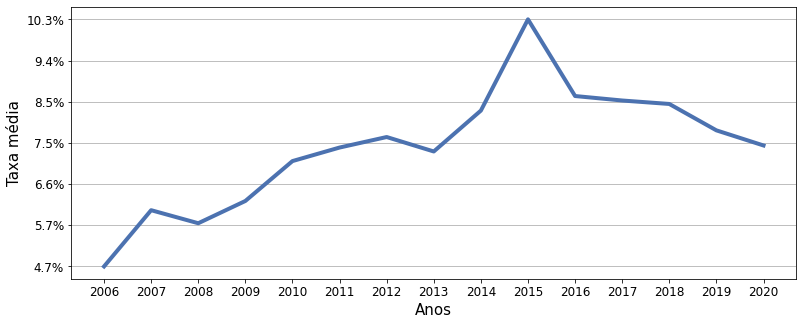
\includegraphics[width=0.45\textwidth]{figuras/taxa_media.png}}
	
	\parbox{\dimexpr\linewidth-2cm}{\raggedright
    \strut \textsuperscript{Fonte: Elaboração própria a partir de dados do Ministério da Agricultura, Pecuária e Abastecimento e da Plataforma
	Atlas do}\strut}\\
    \parbox{\dimexpr\linewidth-2cm}{\raggedright
    \strut \textsuperscript{Seguro Rural \cite{brasil21b}.}\strut}
\end{figure}

Os valores da soma da importância segurada em milhões de reais são apresentados no gráfico da Figura \ref{total_segurado_mil}. Observa-se que há crescimento dos valores segurados, com destaque para o crescimento entre os anos de $2019$ e $2020$, em que o os valores mais que duplicaram. Considerando o período entre $2006$ e $2020$, o crescimento da importância segurada foi de $15,55$ vezes o valor de $2006$. Também é possível observar que, entre os anos de $2014$ e $2015$, ocorreu uma queda de $70,68\%$ do valor segurado.  

Em $2020$, o Programa de Subvenção ao Prêmio do Seguro Rural (PSR) aplicou R\$ $880$ milhões, ou seja, o dobro do valor executado no ano de  $2019$. Para o ano de $2021$, a estimativa apresentada pelo Ministério da Agricultura e Abastecimento foi um aumento de R\$ $1$ bilhão a verba destinada ao PSR \cite{brasil21b}.

No ano de $2014$, o total segurado chegou a R$\$18.462,88$ milhões, no entanto, em $2015$ a soma da importância caiu para R$\$5.398,54$ milhões, o terceiro valor mais baixo do período. O valor mais alto ocorre no ano de $2020$, em que o valor segurado foi de R$\$45,7$ bilhões, o maior desde o início do programa em $2005$.

O valor da importância segurada alcançou $R\$14,4$ bilhões até o mês de junho de $2021$. Este valor é o quinto maior valor da série e já é maior que $25\%$ dos valores registrados nos anos anteriores \cite{brasil21b}. 

%\subsubsection{Área segurada em hectares}

A Figura \ref{area_segurada} apresenta o total da área segurada em hectares nos municípios do Brasil entre os anos de  $2006$ e  $2020$. É possível observar que, a área agrícola segurada no país praticamente dobrou entre $2019$ e $2020$, quando alcançou o maior valor, $13,7$ milhões de hectares, o que representou $20\%$ da área total agrícola do país. O aumento de área em relação a $2019$ é de $98\%$. O maior valor registrado em anos anteriores foi em $2014$, quando foram segurados $9,4$ milhões de hectares. No ano de $2021$, até o mês de junho, foram segurados cerca de $3,76$ milhões de hectares. Esse valor representa cerca de $71,76\%$ da área segurada em $2020$ \cite{brasil21b}. 

%\subsubsection{Indenizações}

Com relação ao número de indenizações,  o gráfico da Figura \ref{apolices_indenizadas} apresenta a evolução das apólices indenizadas ao longo do período analisado. O menor número de indenizações é $389$ em $2006$ e o maior valor ocorreu no ano de $2018$, sendo igual a $17.625$ indenizações. Durante o período, ocorre em média um número de $8.110$ apólices indenizadas por ano, sendo que o crescimento no número de apólices indenizadas foi de $23,31$ vezes entre $2006$ e $2019$. 

Os valores pagos como indenização entre os anos de $2006$ e $2019$ são apresentados no gráfico da Figura \ref{valor_indenizacoes} e variam entre R\$ $20.699.785,74$ em $2006$ e R\$ $924.988.210,45$ em $2018$. A média do valor das indenizações foi de R\$ $345.525.736,50$ no período analisado. 

%\begin{small}
%    \begin{table}[H]
%        \caption{Número de apólices de seguro rural indenizadas por regiões. Brasil $2006-2019$}\label{premio_regioes}
%         \input{../anexos/ap_indeniz_regioes.tex}
%    \end{table}
%\end{small}

%\subsubsection{Taxa média de contratação de seguro rural}

O gráfico apresentado na Figura \ref{taxa_media} mostra a trajetória da taxa de contratação do seguro rural. É possível constatar que a taxa se eleva, em média, de $4,7\%$ em $2006$ para $ 7,46\%$ em $2020$. Até o mês de junho de $2021$, o valor da taxa média havia alcançado $9,79\%$, o segundo maior valor da série, sendo superado pela taxa média cobrada em $2015$, que foi de $10,3\%$ \cite{brasil21b}.  

Segundo Santos e Silva (2017), espera-se que, à medida que o sistema de seguro rural se consolida, reduzam-se os preços das apólices devido aos ganhos de produtividade agropecuária e da redução de fatores de risco. Essas reduções podem ocorrer devido à adoção das orientações do zoneamento agrícola, de um maior conhecimento do histórico de eventos climáticos e dos sinistros ocorridos e, até mesmo em função da adoção de tecnologias, como o uso de irrigação etc. No entanto, essa redução das taxas não ocorreu no período analisado, como observado na Figura \ref{taxa_media}. 

%\begin{figure}[H]
%	\centering
%	\caption{Taxa média anual de contratação do prêmio de seguro rural. Brasil $2006 - 2020$}
%	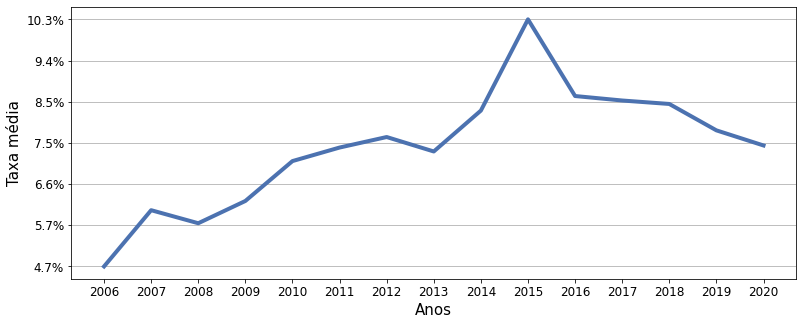
\includegraphics[width=0.8\textwidth]{figuras/taxa_media.png}\\
%	\small \textsuperscript {Fonte: Elaboração própria a partir de dados da Plataforma Atlas do Seguro Rural (Mapa, 2021).}
%   \label{taxa_media}
%\end{figure}

%\begin{small}
%\begin{table}[H]
%\caption{Taxa média de contratação do prêmio de seguro rural por regiões.  Brasil $2006-2020$}\label{tx_media_regioes}
% \input{../anexos/tx_media_regioes.tex}
%\end{table}
%\end{small}

%\subsubsection{Culturas}

A Figura \ref{percent_cult_apol} apresenta o percentual da participação das maiores culturas no número de apólices de seguro rural contratadas. A análise desse gráfico permite identificar que, com exceção de $2015$, a cultura da soja foi a que mais contratou seguro rural. Além disso, observa-se que o milho 2ª safra \footnote{Nesse caso o milho de 2ª safra é listado em separado devido aos distintos graus de risco em relação à 1ª safra \cite{santos17}.} tem cada vez mais aumentado sua participação no número de apólices contratadas. O milho 1ª safra, por sua vez, tem participação que varia entre $1,23\%$ e $16,46\%$, com média de  $6,16\%$ ao longo do período. A participação da cultura da maçã na contratação de seguro rural permanece relativamente estável ao longo do período, variando entre $8,79\%$ e $14,72\%$. 

\begin{figure}[H]
	\centering
	\caption{Percentual da participação das maiores culturas no número de apólices de seguro rural contratadas. Brasil $2006 - 2019$}
    	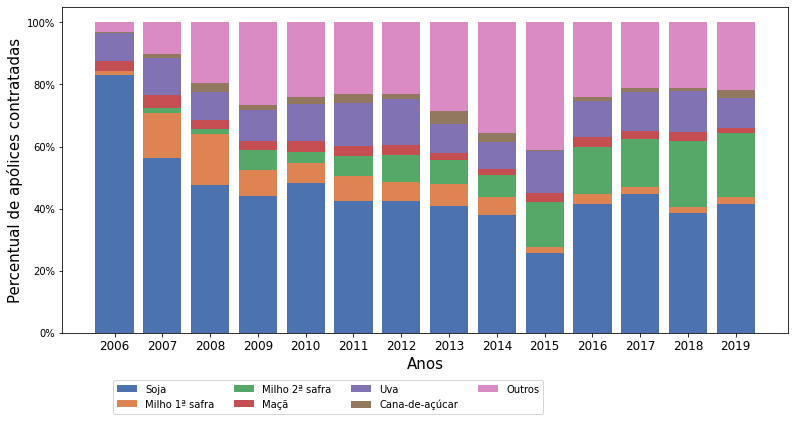
\includegraphics[width=0.8\textwidth]{figuras/percent_apolic_cult.png}\\
	%\small \textsuperscript {Fonte: Elaboração própria a partir de dados do Ministério da Agricultura, Pecuária e Abastecimento \cite{brasil21b}}
	\parbox{\dimexpr\linewidth-2.8cm}{\raggedright
    \strut \textsuperscript{Fonte: Elaboração própria a partir de dados do Ministério da Agricultura, Pecuária e Abastecimento \cite{brasil21b}.}\strut}
    \label{percent_cult_apol}
\end{figure}

A Tabela \ref{percent_culturas} apresenta a participação percentual de grupos de culturas em variáveis do seguro rural. É possível constatar que entre os anos de $2006$ e $2020$, as culturas de grãos foram responsáveis por $74,85\%$ das apólices contratadas, seguida das culturas de frutas com $14,74\%$ das apólices no período. Em terceiro lugar está a cultura de olerícolas, com cerca de $3,36\%$ de participação na contratação de apólices de seguro rural. Uma estrutura semelhante de participação percentual de grupos de culturas pode ser observada com relação à participação no valor total segurado. O grupo de cultura que mais se destaca é a dos grãos, com $74,88\%$ do total segurado, seguido das frutas e do café, com $9,55\%$ e $4,04\%$, respectivamente. 

\begin{small}
\begin{table}[H]
\caption{Participação percentual das culturas nos valores do seguro rural. Brasil $2006-2020$}\label{percent_culturas}
 \footnotesize
\vspace{0.05cm}
\begin{tabularx}{\textwidth}{lRRRRR}
    \hline \\[-1.9ex]	 
    Cultura    & \% das apólices & \% do total segurado & \% do premio total & \% de subvenção & Taxa média \\
    \hline \\[-1.9ex]	 
    Grãos      & 74,85\%         & 74,88\%              & 78,86\%            & 77,35\%         & 7,70\%     \\
    Frutas     & 14,74\%         & 9,55\%               & 13,14\%            & 16,07\%         & 9,17\%     \\
    Olerícolas & 3,36\%          & 2,74\%               & 3,17\%             & 2,85\%          & 7,64\%     \\
    Café       & 3,07\%          & 4,04\%               & 2,19\%             & 1,61\%          & 3,15\%     \\
    Cana       & 2,08\%          & 2,98\%               & 0,77\%             & 0,69\%          & 1,63\%     \\
    Pecuária   & 0,73\%          & 1,16\%               & 0,77\%             & 0,32\%          & 3,26\%     \\
    Floresta   & 0,30\%          & 3,51\%               & 0,42\%             & 0,35\%          & 1,60\%     \\
    Outros     & 0,88\%          & 1,13\%               & 0,68\%             & 0,75\%          & 4,64\%     \\ 
    \hline 
\end{tabularx}
%\vspace{0.5cm}
\small \textsuperscript{Fonte: Elaboração própria a partir de dados da Plataforma Atlas do Seguro Rural (Mapa, 2021).  }\\
\end{table}
\end{small}

Além disso, é possível observar na Tabela \ref{percent_culturas}, os percentuais de subvenção ao prêmio de seguro rural e os valores da taxa média de contratação do seguro. As taxas cobradas durante o período para a cultura de grãos foi de $7,70\%$, a taxa cobrada das culturas de frutas foi de $9,17\%$ e as olerícolas tiveram uma taxa média de contratação de $7,64\%$. Os percentuais de subvenção dessas culturas são, também, os mais altos: $77,35\%$ de subvenção para os grãos, $16,07\%$ para as culturas de frutas e $2,85\%$ para as olerícolas. Ou seja, os grupos de culturas com maior demanda pelo seguro, além de apresentarem os maiores valores de apólices, os maiores valores e maior ocorrência de sinistros, são também aqueles com maiores taxas médias. 

De acordo com  Santos e Silva (2017), este fato pode apontar para a possibilidade de dois fenômenos a serem melhor examinados. O primeiro diz respeito à situação em que as maiores taxas resultam do fato de que maiores subvenções são dadas a cultivos de maior risco. O segundo fenômeno possível é que as taxas sejam mais altas, principalmente no caso dos produtores que adotam o ZARC, com elevada tecnologia produtiva, alta produtividade e não têm estas características levadas em consideração como informação que contribui para a redução das taxas. Dessa forma, se por um lado o seguro agrícola não se consolida sem a subvenção dada pelo Estado, por outro, é possível que esse sistema de subvenção ao prêmio crie distorções no mercado de seguro rural. 

%\subsubsection{Seguradoras}

A Tabela \ref{seguradoras} exibe a distribuição das fatias de mercado das seguradoras entre $2006$ e $2020$. Apesar de as seguradoras passarem de cinco, em $2006$, para $16$ companhias aptas a operar com seguro rural em $2020$, é possível constatar que há uma concentração do mercado de seguro em um número reduzido de seguradoras. 

\begin{small}
\begin{table}[H]
\caption{Participação de mercado das seguradoras. Brasil $2006-2020$}\label{seguradoras}
 \footnotesize
\vspace{0.05cm}
\begin{tabularx}{\textwidth}{lRRRRRRR}
    \hline \\[-1.9ex]	 
    Seguradora         & Apólices        & \% do número de apólices  & Beneficiários  & \% dos beneficiários  & Área segurada (em mil ha)  & \% de área segurada   \\
    \hline \\[-1.9ex]	 
    Brasilseg         &  $410.892$      &  $37,23  $                &  $95.769$                    &  $26,85  $            &  $48.076,26$       & $55,31  $              \\
    Mapfre            &  $149.389$      &  $13,54  $                &  $49.274$                    &  $13,82  $            &  $7.309,17$        &  $8,41  $               \\
    Essor             &  $119.087$      &  $10,79  $                &  $38.995$                    &  $10,93  $            &  $4.603,47$        &  $5,30  $               \\
    Swiss Re          &  $91.410$       &  $8,28  $                 &  $34.483$                    &  $9,67  $             &  $7.870,31$        &  $9,06  $               \\
    Nobre             &  $82.500$       &  $7,48  $                 &  $29.053$                    &  $8,15  $             &  $2.747,88$        &  $3,16  $               \\
    Allianz           &  $66.983$       &  $6,07  $                 &  $21.210$                    &  $5,95  $             &  $5.387,98$        &  $6,20  $               \\
    Sancor            &  $49.567$       &  $4,49  $                 &  $22.516$                    &  $6,31  $             &  $3.210,37$        &  $3,69  $               \\
    Fairfax           &  $35.343$       &  $3,20  $                 &  $18.349$                    &  $5,14  $             &  $2.055,87$        &  $2,37  $               \\
    Porto Seguro      &  $26.306$       &  $2,38  $                 &  $6.152$                     &  $1,72  $             &  $259,33$          &  $0,30  $               \\
    Newe              &  $22.741$       &  $2,06  $                 &  $12.337$                    &  $3,46  $             &  $1.469,10$        &  $1,69  $               \\
    Tokio Marine      &  $19.808$       &  $1,79  $                 &  $11.263$                    &  $3,16  $             &  $1.722,64$        &  $1,98  $               \\
    Too               &  $14.844$       &  $1,35  $                 &  $9.768$                     &  $2,74  $             &  $1.163,48$        &  $1,34  $               \\
    Aliança do Brasil &  $7.200$        &  $0,65  $                 &  $3.294$                     &  $0,92  $             &  $593,19$          &  $0,68  $               \\
    Excelsior         &  $4.472$        &  $0,41  $                 &  $2.292$                     &  $0,64  $             &  $238,97$          &  $0,27  $               \\
    Sompo             &  $3.062$        &  $0,28  $                 &  $1.901$                     &  $0,53  $             &  $181,66$          &  $0,21  $               \\
    Itaú              &  $9$            &  $0,00  $                 &  $9$                         &  $0,00  $             &  $25,10$           &  $0,03  $               \\
    \hline \\[-1.9ex]
    \textbf{Total}    & \textbf{1.103.613} & \textbf{100  }         & \textbf{213.692}             & \textbf{100  }        & \textbf{86.914,79} & \textbf{100  }\\
	\hline 
\end{tabularx}
%\vspace{0.5cm}
\small \textsuperscript{Fonte: Elaboração própria a partir de dados da Plataforma Atlas do Seguro Rural (Mapa, 2021).}\\
\footnotesize{Nota: Valores acumulados $2006 -- 2020$}\\
\end{table}
\end{small}

Ao se analisar a participação no percentual do número de apólices de seguro rural, percebe-se que apenas as três maiores seguradoras (Brasilseg, Mapfre e Essor) concentram cerca de $61,56\%$ do mercado. Com relação ao percentual dos beneficiários, as três maiores seguradoras contam com cerca de $51,60\%$ dos beneficiários durante o período analisado. A concentração é ainda maior quando se analisa o percentual da área segurada, sendo que a  maior seguradora do ramo (Brasilseg) conta com um percentual de $55,31\%$ da área segurada em hectares. As três maiores seguradoras são responsáveis pelo seguro de $72,78\%$ da área segurada. 

%A próxima seção tem como objetivo apresentar os resultados da análise da distribuição espacial dos dados do seguro rural no Brasil. 

\subsection{A DISTRIBUIÇÃO REGIONAL DO SEGURO RURAL} 

Os gráficos apresentados na Figura \ref{variaveis_regioes} exibem a evolução, entre os anos de $2006$ e $2019$, das variáveis de seguro rural analisadas por regiões.

Na figura \ref{ap_contrat_regioes}, é possível observar a evolução do número de apólices contratadas nas regiões brasileiras. Na Figura \ref{ap_contrat_regioes}, observa-se que a região Sul se destaca das demais com relação ao número de apólices contratadas. O menor número de apólices contratadas na região Sul foi de $16.525$ apólices no ano de $2006$. O valor médio de apólices contratadas durante o período foi $44.166$ apólice. No ano de $2014$, foi registrado o maior número de apólices contratadas ($76.668$ apólices). 

% variaveis_regioes
\begin{figure}[H]
	\centering
	\caption{Evolução das variáveis de seguro rural por regiões. Brasil $2006 - 2019$}\label{variaveis_regioes}
	\small
	
	\subfloat[Número de apólices contratadas\label{ap_contrat_regioes}]{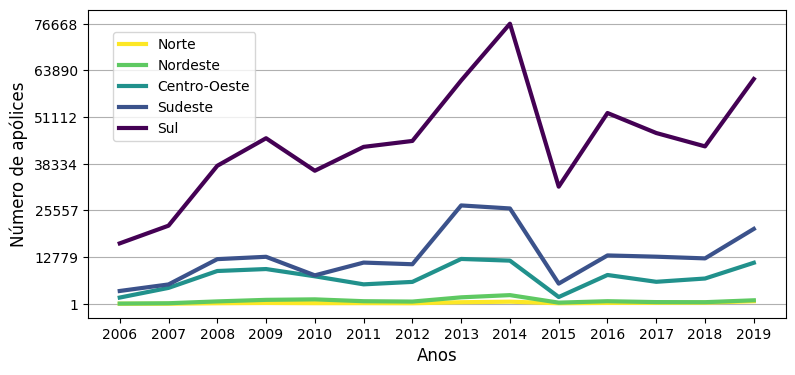
\includegraphics[width=0.45\textwidth]{figuras/ap_contrat_regioes.png}}\hspace{0.1cm}
	\subfloat[Total segurado (em milhões de R\$)\label{t_segurado_regioes}]{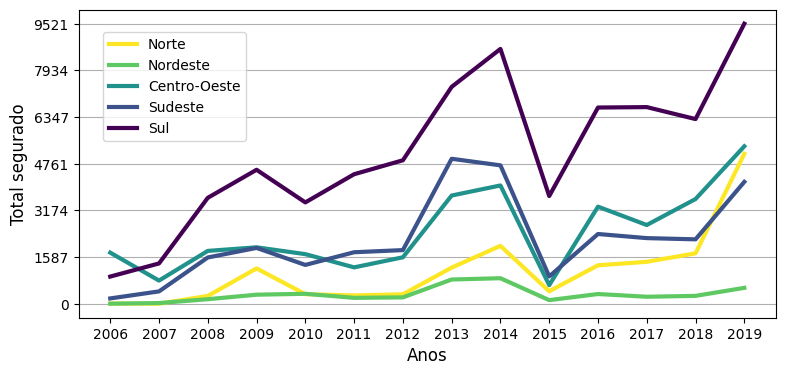
\includegraphics[width=0.45\textwidth]{figuras/t_segurado_regioes.png}}\\
	
	\subfloat[Valores de prêmio (em milhões de R\$)\label{soma_premio_regioes}]{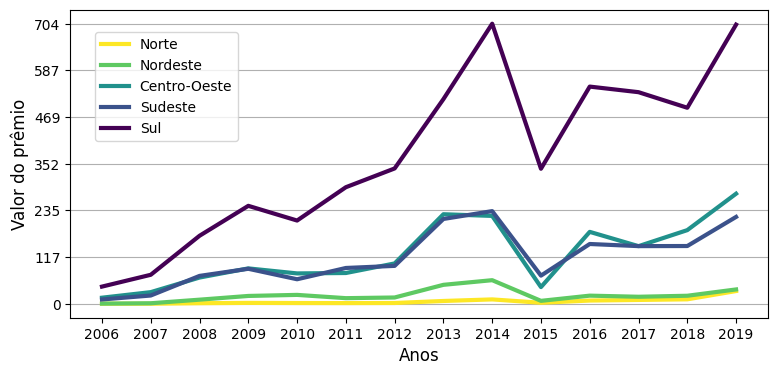
\includegraphics[width=0.45\textwidth]{figuras/soma_premio_regioes.png}}\hspace{0.1cm}
	\subfloat[Valores subvenção (em milhões de R\$)\label{t_subvencao_regioes}]{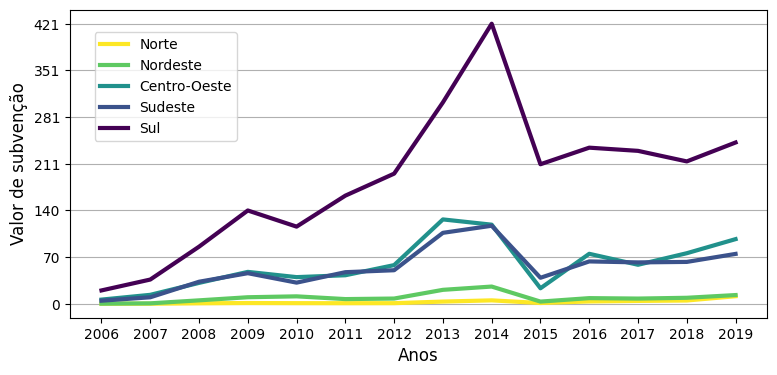
\includegraphics[width=0.45\textwidth]{figuras/t_subvencao_regioes.png}}\\
	
	\subfloat[Apólices indenizadas\label{ap_indeniz_regioes}]{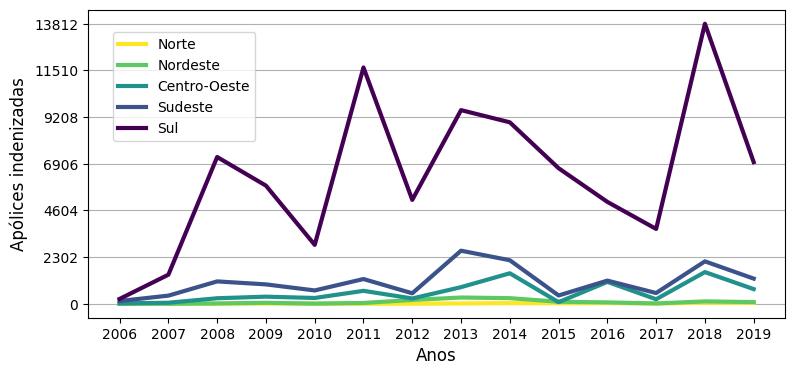
\includegraphics[width=0.45\textwidth]{figuras/ap_indeniz_regioes.png}}\hspace{0.1cm}
	\subfloat[Valor das indenizações (em milhões de R\$)\label{inde_pagas_regioes}]{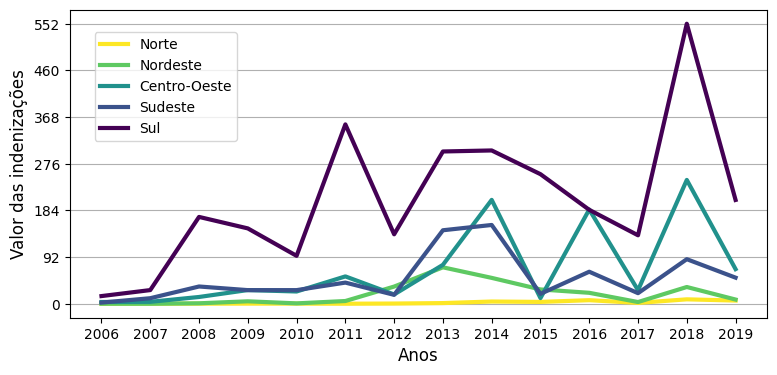
\includegraphics[width=0.45\textwidth]{figuras/inde_pagas_regioes.png}}\\
	
    \parbox{\dimexpr\linewidth-2cm}{\raggedright
    \strut \textsuperscript{Fonte: Elaboração própria a partir de dados do Ministério da Agricultura, Pecuária e Abastecimento \cite{brasil21b}}\strut}
\end{figure}

A segunda região com maior número de apólices contratadas é a região Sudeste (Figura \ref{ap_contrat_regioes}). Em média, na região Sudeste, foram contratadas $12.942$ apólices por ano, o maior valor registrado foi $26.913$ apólices contratadas em $2013$. A região Centro-Oeste é a terceira região com mais apólices contratadas, sendo que em média foram contratadas $7.225$  por ano e, em $2013$ foi registrado o maior número de apólices ($12.260$). Por fim, as regiões Norte e Nordeste, apresentaram respectivamente, em média, $240$ e $804$ apólices contratadas por ano.

A taxa de crescimento do número de apólices contratadas na região sul foi de $3,72$ vezes o valor inicial entre os anos $2006$ e $2019$. Por sua vez, durante o período analisado a região Sudeste teve um crescimento do número apólices de $5,87$ vezes e a região Centro-Oeste apresentou um crescimento do número de apólices de $6,66$ vezes. As regiões Norte e Nordeste apresentaram um crescimento médio anual igual a $0,14\%$ e $4,04\%$ respectivamente. 

Ao se analisar a evolução do total segurado nas regiões brasileiras apresentado na Figura \ref{t_segurado_regioes}, é possível observar que a região Sul se destaca com, em média, $5146,83$ milhões de valor segurado total. O maior valor foi registrado em $2019$ e foi igual a $9520,85$ milhões, o segundo maior valor foi igual a $8664,31$ milhões e foi registrado em $2015$. 

No início da série valores a região Centro-Oeste apresenta um maior valor total segurado do que a região Sul (5.355 milhões). Além disso, como é possível observar na Figura \ref{t_segurado_regioes}, a partir do ano de $2016$ a região Centro-Oeste supera a região Sudeste no valor total segurado. A região Norte apresentou, com relação ao total segurado, os valores de $120,35$ milhões em $2009$ e $197,01$ milhões em $2014$. 
Além disso, a região Norte apresenta o seu maior valor no ano de $2019$, com total segurado igual a $509,94$ milhões. Também é possível observar que há indícios de haver um crescimento do total segurado em todas as regiões. 

O total segurado na região Sul apresenta um crescimento de cerca de $10,27$ vezes entre os anos de $2006$ e $2019$. Na região Sudeste, o crescimento foi de $22,52$ vezes o valor registrado em $2006$. Por sua vez, o Centro-Oeste apresentou um crescimento de cerca de $3,07$ vezes o valor do total segurado durante o período. O valor do total segurado na região Norte cresceu $499.51$ vezes entre os anos $2006$ e $2019$. Por fim, no Nordeste, o valor total segurado apresentou um crescimento de $106,95$ vezes o valor inicial. 

Para mais, ao se analisar a Figura \ref{soma_premio_regioes} e \ref{t_subvencao_regioes}, é possível observar que as variáveis valores de prêmio e valores subvenção apresentam crescimento durante o período analisado. Também é possível observar que, com exceção das variáveis relacionadas à indenização, as variáveis apresentam uma queda entre os anos de $2014$ e $2015$.

É possível observar na Figura \ref{ap_indeniz_regioes}, que a região Sul se destaca quando se analisa o número de apólices indenizadas. Os valores variam de $237$ em $2006$ e $13812$ apólices indenizadas em $2019$. Em média, a região Sul teve cerca de $6364$ apólices indenizadas durante o período. Além disso, durante os anos analisados, houve um crescimento de $58,28\%$ no número de apólices de seguro rural indenizadas. A região Sudeste é a segunda região com maior número de apólices indenizadas, sendo que o menor número de apólices indenizadas na região Sudeste foi de $135$ e ocorreu em $2006$, com maior valor registrado em $2013$, equivalente a $2.616$. 

Ao longo dos anos analisados, a diferença entre o número de apólices na região Sul e Sudeste foi em média igual a $5.283$ apólices. A região Centro-Oeste foi responsável por, em média, $559,64$ apólices indenizadas. O maior número de apólices indenizadas na região Centro-Oeste foi registrado em $2018$ e foi igual a $1561$ apólices. As regiões Norte e Nordeste tiveram em média $15,57$ e $88,64$, respectivamente. 

Com relação ao valor das indenizações de seguro rural pagas, é possível observar na Figura \ref{inde_pagas_regioes}, que a região Sul é a que possui os maiores valores pagos como indenização. Em média, foram pagos R$\$205,66$ milhões como indenização. O maior valor foi equivalente a R$\$551,74$ milhões e foi registrado em $2018$ e o menor valor foi registrado no primeiro ano analisado, sendo equivalente a R$\$15.06$ milhões. 

A Tabela \ref{media_regioes} apresenta a média dos valores anuais das variáveis de seguro rural acumulados por regiões no Brasil no período de $2006$ e $2019$. Como é possível observar, que a região Sul se destaca das demais com os maiores valores das médias das variáveis. Com relação ao número de apólices contratadas, a segunda região com maior média da variável total de apólices contratadas é o Sudeste. No entanto, quando se analisa a média da soma da importância seguradas, a segunda região com maior média é a região Centro-Oeste. A região Centro-Oeste, também conta com maiores médias nas variáveis soma dos prêmios pagos, total da subvenção e soma das indenizações pagas com relação às regiões Norte, Nordeste e Sudeste. A região Sudeste apresenta a maior média anual do número de apólices indenizadas. 



\begin{small}
\begin{table}[H]
\caption{Média anual dos valores das variáveis de seguro rural por regiões. Brasil $2006-2019$}\label{media_regioes}
\begin{center}
\footnotesize
    \begin{tabular}{lrrrrr}
    \hline \\[-1.9ex]	
    Variável                                  & Norte   & Nordeste & Centro-Oeste & Sudeste  & Sul       \\
    \hline \\[-1.9ex]	
    Total de apólices contratada              &  240,14 &   803,57 &      7.225,36 &  12.941,5 &  44.166,14 \\
    Soma da importância segurada (R\$ milhão) &   111,5 &   319,82 &      2.428,79 &  2.178,54 &   5.146,84 \\
    Soma dos prêmios (R\$ milhão)             &    6,37 &    20,76 &       123,43 &   115,02 &    371,72 \\
    Total de subvenção (R\$ milhão)           &    2,66 &     9,25 &        58,25 &    53,52 &    186,56 \\
    Soma das indenizações pagas (R\$ milhão)  &    2,39 &    18,73 &        68,59 &    50,15 &    205,66 \\
    Taxa média aplicada às apólices           &    0,01 &     0,01 &         0,13 &     0,11 &      0,45 \\
    Número de apólices indenizadas            &   15,57 &    88,64 &       559,64 &  1.081,57 &   6.364,57 \\
    \hline 
    \end{tabular}
\end{center}
\small \textsuperscript {Fonte: Elaboração própria a partir de dados do Ministério da Agricultura, Pecuária e Abastecimento (MAPA)}\\


\end{table}
\end{small}

A média dos valores anuais da taxa média de contratação de apólices indica que, a região Sul é a que possui maior taxa de contratação de seguro com taxa média igual a $0,45$ ao longo dos anos. A região Centro-Oeste é a que tem o segundo maior valor de taxa média durante os anos, sendo igual a $0,13$. As regiões Norte e Nordeste apresentaram taxa média igual a $0,01$.

\subsection{DISTRIBUIÇÃO ESPACIAL DO SEGURO RURAL}

A análise da distribuição espacial das variáveis se inicia com a visualização dos mapas temáticos. Por meio destes mapas, busca-se identificar visualmente se há a ocorrência de padrões na distribuição espacial das variáveis do seguro rural.

O primeiro grupo de mapas, apresentado na Figura \ref{map_segurado}, exibe a distribuição espacial da soma da importância segurada (R\$ milhão) nos municípios brasileiros entre os anos de $2006$ e $2019$. Para a construção dos mapas, os valores da variável foram divididos em 5 intervalos \footnote{Para a criação dos intervalos foi aplicado algoritmo Fisher Jenks aos valores das variáveis diferentes de $0$ e os intervalos foram criados tendo como referência os valores do ano de 2019 \cite{jenks77}}.

\begin{figure}[H]
	\centering
	\caption{Total segurado por municípios (em mil R\$). Brasil $2006 - 2019$}
	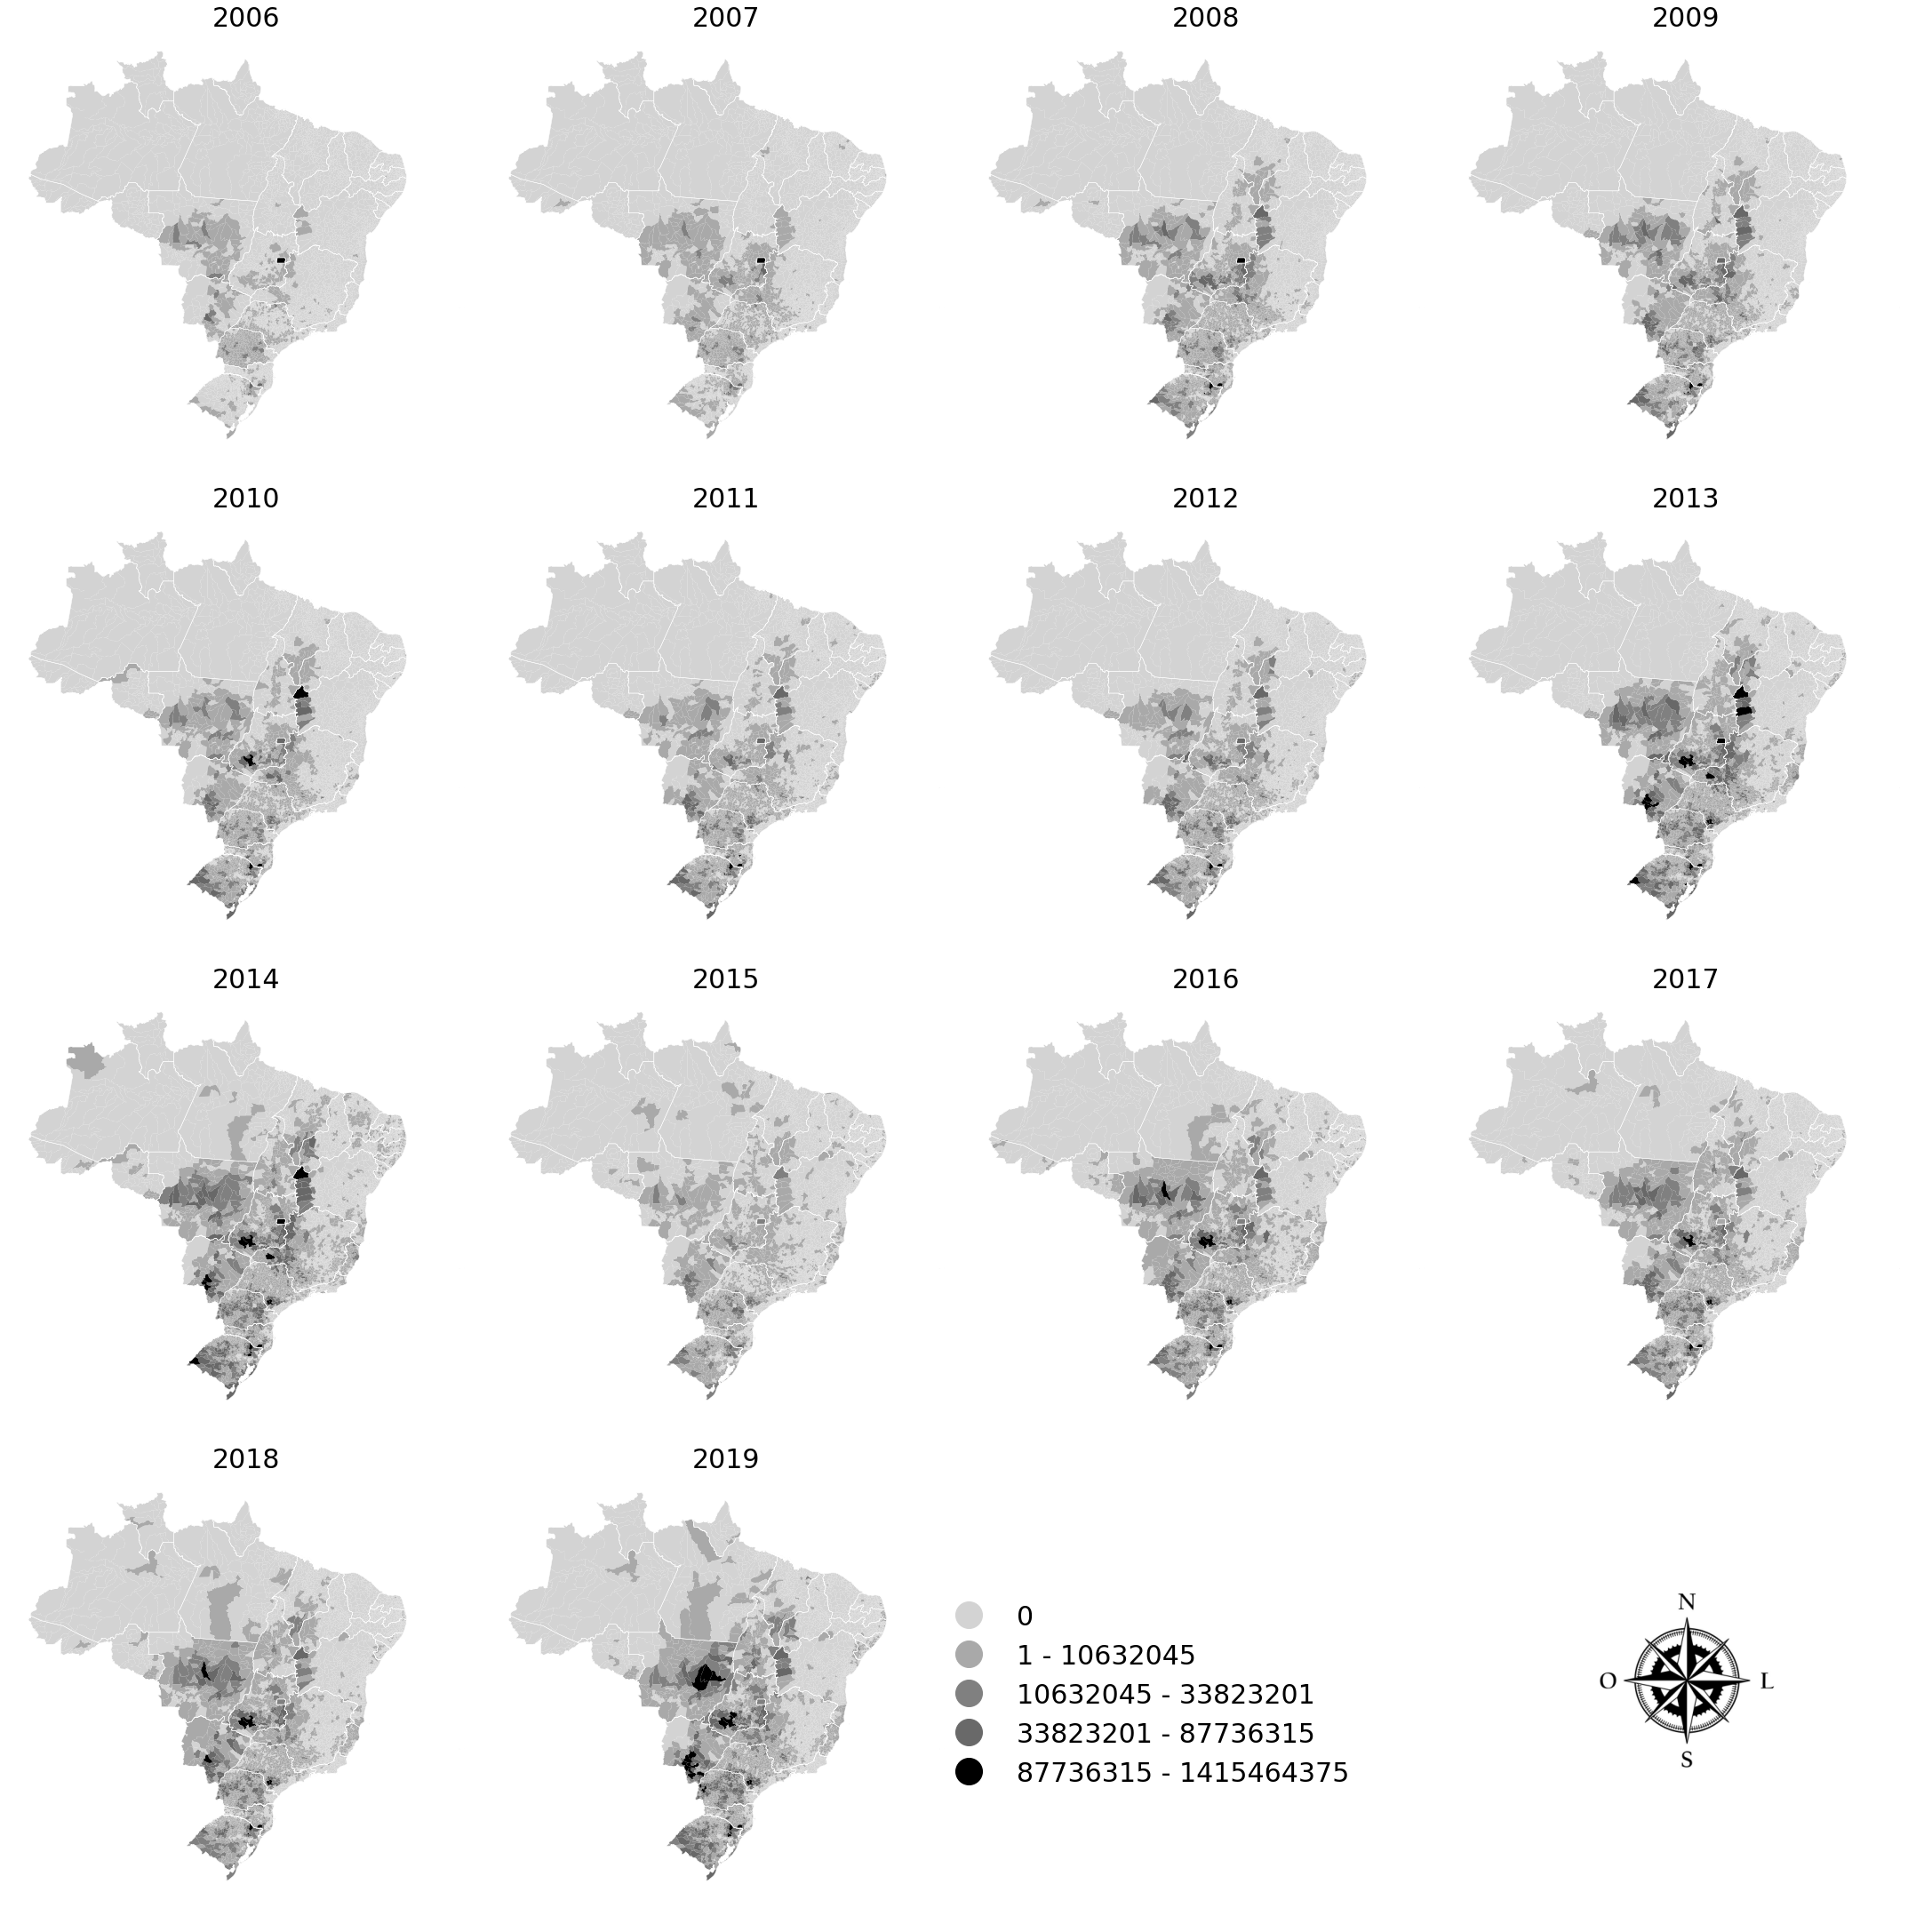
\includegraphics[width=0.9\textwidth]{figuras/map_total_segurado_mil.png}
	\small \textsuperscript {Fonte: Elaboração própria a partir de dados do Ministério da Agricultura, Pecuária e Abastecimento \cite{brasil21b}}
    \label{map_segurado}
\end{figure}

Pela análise da Figura \ref{map_segurado}, é possível observar que a distribuição espacial do total segurado se modificou no decorrer dos anos, apesar de se concentrar principalmente nas Regiões Sul e Centro-Oeste. É possível também destacar que, durante o período analisado, há indícios de concentrações espaciais na região do Extremo Oeste Baiano no Estado da Bahia, Sudoeste de Mato Grosso do Sul, Sul Goiano no Estado de Goiás e Sudeste, no sul do Estado de São Paulo.

O conjunto de mapas apresentado na Figura \ref{map_apolices}, exibe o número de apólices de seguro rural contratadas por municípios entre $2006$ e $2019$. Ao longo dos anos, o número de municípios com nenhuma apólice contratada cai e há indícios de um aumento do número de apólices até o ano de $2014$. Entre os anos de $2014$ e $2015$, há uma queda no número de apólices contratadas, como já foi mostrado no gráfico da Figura \ref{apolices_produtores}, e das demais variáveis relacionadas ao seguro rural. Essa redução também pode ser visualizada no mapa da Figura \ref{map_apolices}, em que o ano de $2015$ apresenta municípios com menor número de apólices contratadas. 

Ao se analisar a distribuição espacial, observa-se que há indícios de haver uma maior concentração espacial do total segurado e do número de apólices de seguro rural contratadas em algumas regiões. A partir do ano de $2015$ a retomada do crescimento destas variáveis (Figura \ref{total_segurado_mil}) pode ser visualizado com um maior número de áreas de coloração mais escura nos mapas (Figuras \ref{map_segurado} e \ref{map_apolices}).

\begin{figure}[H]
	\centering
	\caption{Número de apólices de seguro rural contratadas por municípios. Brasil $2006 - 2019$}
	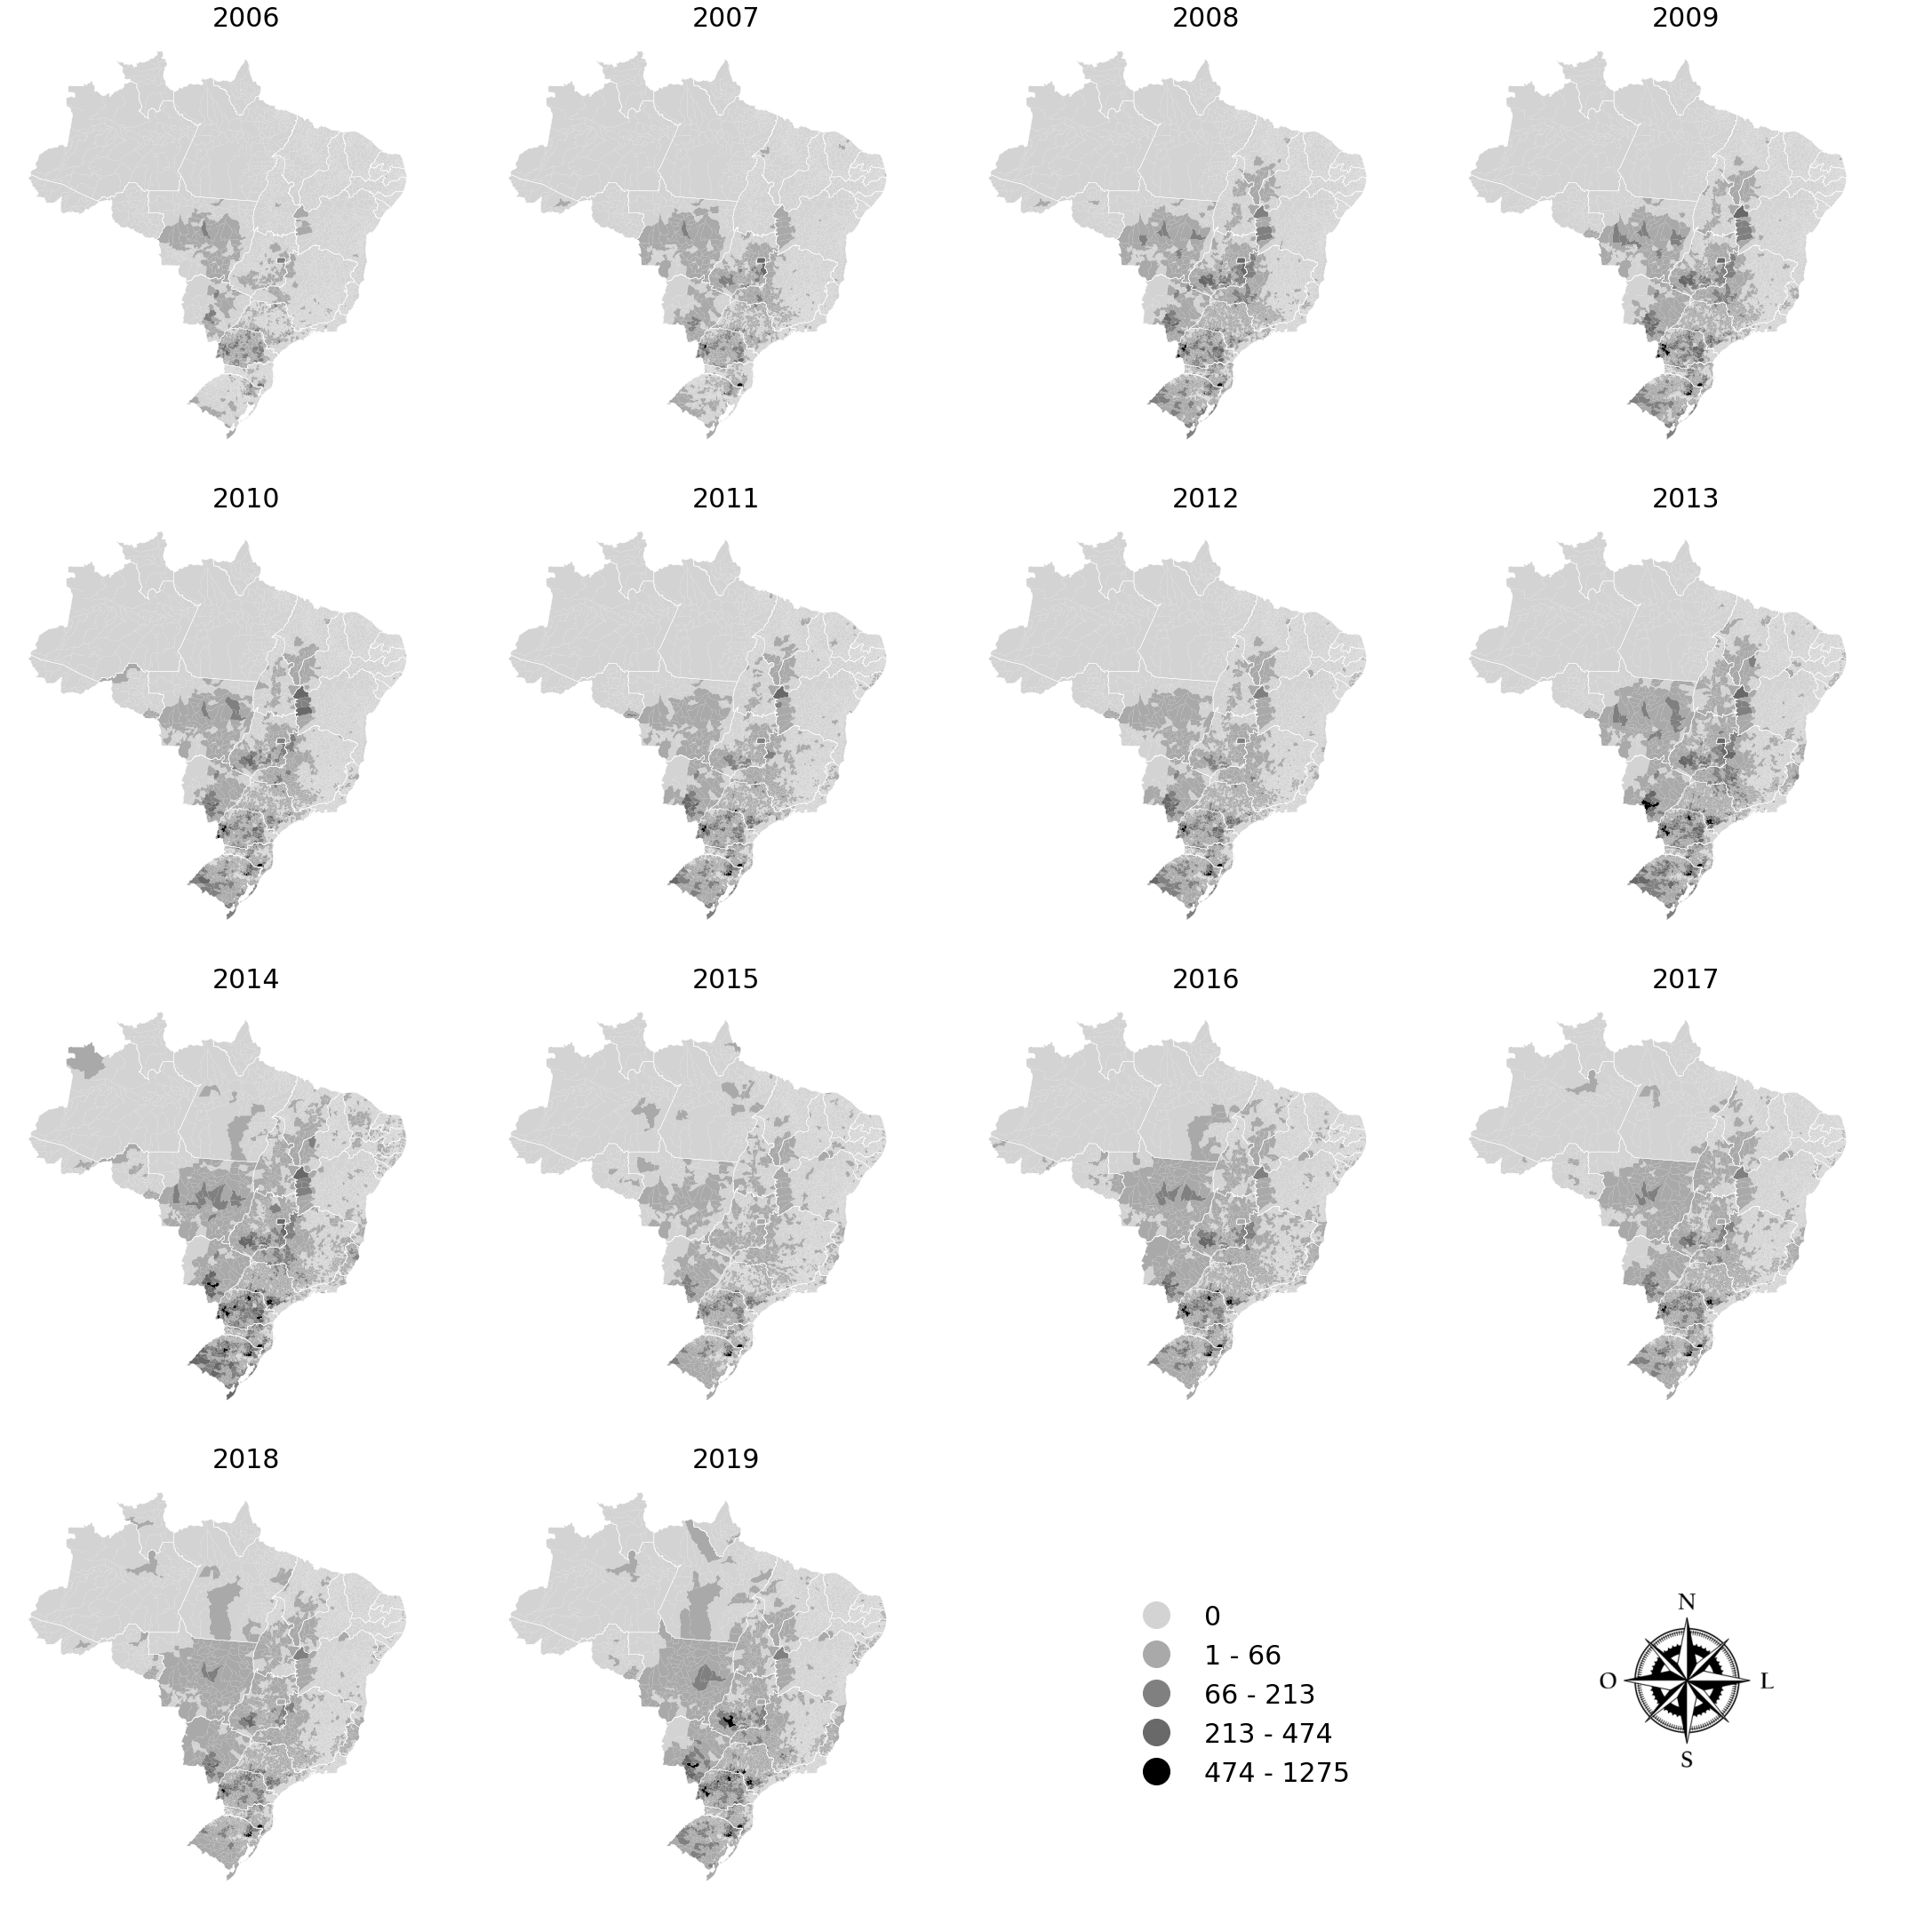
\includegraphics[width=0.9\textwidth]{figuras/map_apolices_contratadas.png}
	\small \textsuperscript {Fonte: Elaboração própria a partir de dados do Ministério da Agricultura, Pecuária e Abastecimento \cite{brasil21b}}
    \label{map_apolices}
\end{figure}

A distribuição espacial das demais variáveis analisadas apresenta um padrão semelhante ao observado com a soma da importância segurada (R\$ milhão)  \footnote{Os mapas da distribuição espacial das variáveis do seguro rural no Brasil são apresentados no apêndice A}. Dessa forma, os resultados corroboram a hipótese apresentada por Silva, Teixeira e Santos (2014) na investigação sobre a participação do PSR na universalização do acesso ao seguro rural. Ou seja, apesar da evolução do seguro rural em âmbito nacional, quando se observa a distribuição espacial, verifica-se que há, ao longo do tempo, uma concentração das apólices e subvenções na região Sul e Centro-Oeste. Portanto, apesar de ter ocorrido uma ampliação do seguro rural, esta ampliação ocorreu de forma concentrada, o que evidencia o cumprimento de forma parcial dos objetivos do PSR \cite{silva14}.

\section{CONSIDERAÇÕES FINAIS}

%O objetivo do presente trabalho foi analisar a evolução e a dinâmica espacial de variáveis do seguro rural nos municípios brasileiros entre 2006 e 2019. Além disso, buscou-se investigar a presença de padrões de distribuição espacial. A

A análise possibilitou constatar resultados positivos na evolução do seguro rural no Brasil. O número de apólices contratadas tem um crescimento de cerca de $8,69$ vezes seu valor inicial durante o período. Ademais, a área agrícola segurada no país praticamente dobrou entre os anos de $2019$ e $2020$, quando alcançou o maior valor, $13,7$ milhões de hectares, que representa $20\%$ da área total agrícola do país. 

Em geral, identificou-se que as maiores concentrações de apólices de seguro rural estão situadas nas regiões Sul, Centro-Oeste e Sudeste, no sul do Estado de São Paulo.  Para mais, ressalta-se que, embora mantenham a concentração do número de apólices contratadas, número de apólices indenizadas, valores de subvenção, indenização e prêmio, atualmente há expansão da demanda por seguros agrícolas. 

Apesar de os dados indicarem uma concentração geográfica da adesão ao sistema de seguro rural no Brasil, é necessário levar em consideração outros sistemas, como o Proagro e o programa Garantia Safra. É necessário, ainda, ressaltar que a adesão dos produtores deve ocorrer como uma resposta à percepção do risco das atividades agropecuárias, ou seja, o seguro deve difundir-se com base na compreensão dos riscos e das vantagens de sua contratação. 

Por fim, este trabalho pode ser entendido como uma abordagem inicial, a partir da qual é possível se introduzir novos métodos estatísticos a fim de aprimorar os resultados. Dentre esses métodos, destaca-se a Análise de Componentes Principais (ACP), que pode ser utilizada para reduzir o número de variáveis,  de forma a possibilitar a incorporação de informação de mais de uma variável na análise exploratória espacial.

\newpage
\addcontentsline{toc}{section}{\hspace*{\distnumber}REFERÊNCIAS}
\begin{center}
\section*{REFERÊNCIAS} 
\end{center}




%%.....................................................
%% inclui referências

\begin{flushleft}
\renewcommand\refname{}
\vspace*{-0.9cm}
\begin{singlespace}
\documentclass[10pt]{article}
%==========================================================================================

\usepackage[utf8]{inputenc}
\usepackage[brazil]{babel}
\usepackage[T1]{fontenc}
\usepackage{amsmath}
\usepackage{amsfonts}
\usepackage{mathrsfs}
\usepackage{amssymb}
\usepackage{graphicx}
\usepackage{geometry, calc, color, setspace}
\usepackage{indentfirst}
\usepackage{wrapfig}
\usepackage{boxedminipage}
\usepackage{enumerate}
\usepackage{float}
\usepackage{paralist}
\usepackage{comment}
\usepackage{icomma}
\usepackage{rotating}
\usepackage{multirow}
\usepackage[position=bottom]{subfig}
\usepackage{array}
\usepackage{tabularx}
\usepackage{float}
\usepackage{array}

\newcolumntype{L}[1]{>{\raggedright\let\newline\\\arraybackslash\hspace{0pt}}m{#1}}
\newcolumntype{C}[1]{>{\centering\let\newline\\\arraybackslash\hspace{0pt}}m{#1}}
%\newcolumntype{R}[1]{>{\raggedleft\let\newline\\\arraybackslash\hspace{0pt}}m{#1}}
\newcolumntype{R}{>{\raggedleft\let\newline\\\arraybackslash\hspace{0pt}}X}

\usepackage[alf,bibjustif]{abntex2cite}
%\usepackage{abntcite}

% Para o alinhamento dos títulos das figuras
\usepackage{caption}
%\captionsetup[figure]{format=hang,labelsep=endash,font=small,justification=RaggedRight,singlelinecheck=off, margin=1cm}
\captionsetup[subfigure]{textfont=small,singlelinecheck=off,justification=raggedright}


%%  Inserindo os códigos Python ==================================
\usepackage{listings}

%\definecolor{light_gray}{rgb}{0.97,0.97,0.97}
%\definecolor{mymauve}{rgb}{0.58,0,0.82}
%\definecolor{mygreen}{rgb}{0,0.6,0}

\lstset{
  language = Python,
  inputencoding = utf8,
  backgroundcolor = \color{white},
  columns=fullflexible,
  basicstyle=\ttfamily,
  breaklines=true,
  postbreak=\raisebox{0ex}[0ex][0ex]{\color{black}$\hookrightarrow$\space},
  keywordstyle=\color{black},      % keyword style
  stringstyle=\color{black},
  commentstyle=\color{black}
}

\newcommand{\HRule}{\noindent\rule{\linewidth}{0.2mm}}

\usepackage{mathpazo}                         % tem suporte matemático
\usepackage[scaled=0.85]{beramono}            % usa esta nos verbatins [scaled=0.9]

\renewcommand\UrlFont{\color{black}\rmfamily} 

\def\distnumber{2.3em}

%==========================================================================================

\author{Walef Machado de Mendonça\footnote{Mestrando em Estatística Aplicada e Biometria na Universidade Federal de Alfenas}\\
Patrícia de Siqueira Ramos\footnote{Professora da Universidade Federal de Alfenas, campus Varginha}}

%==========================================================================================


\title{O seguro rural no Brasil: evolução e distribuição espacial}

\date{}

\begin{document}

\maketitle

\begin{abstract}
As atividades agropecuárias se inserem em um contexto de adversidades que as colocam em situação diferenciada em relação aos riscos enfrentados pelos produtores. Tais atividades demandam grandes investimentos, o que faz com que sua atratividade esteja relacionada às formas existentes de gerenciamento de riscos. Uma das formas mais usuais de gerenciamento de risco neste setor é a contratação de Seguro Rural, uma vez que esta modalidade de seguro possibilita a recuperação da capacidade financeira do produtor na ocorrência de sinistros. Nesse sentido, o objetivo do trabalho é avaliar a distribuição e a dinâmica espacial de variáveis relacionadas às apólices de Seguro Rural contratadas nos municípios brasileiros no período de 2006 a 2019. Além disso, busca-se investigar a existência de dependência espacial e a presença de agrupamentos com grande número de apólices de Seguro Rural. Para tanto, utiliza-se os dados dos Censos do Seguro Rural, compilados pelo Ministério da Agricultura, Pecuária e Abastecimento (MAPA) e Análise Exploratória de Dados Espaciais (AEDE). Os resultados apontam que as maiores concentrações de apólices de Seguro Rural estão situadas nas regiões Sul e Centro-Oeste. Além disso, apesar de haver um aumento nas contratações de Seguro Rural, há também uma tendência de maior concentração espacial das apólices ao longo do período analisado. \\
\newline
\noindent {\textbf{Palavras-chave}}: Seguro rural. Política agrícola. Estatística espacial. Autocorrelação espacial. I de Moran.
\end{abstract}

\section{INTRODUÇÃO}

O setor agropecuário brasileiro tem se destacado nas últimas décadas por seu crescimento proveniente da aplicação de novas tecnologias ao clima tropical e a incorporação de novas áreas de terras \cite{brasil19a}. Segundo dados dos censos agropecuários, entre $2006$ e $2017$, tanto a área total quanto a produção agrícola e pecuária vivenciaram crescimento. Neste período houve um acréscimo de cerca de $5,8\%$ na área total dos estabelecimentos agropecuários \cite{ibge19}. Com relação à sua participação no PIB, em 2019, a parcela do agronegócio brasileiro foi de  $20,5\%$  do PIB nacional. Já em 2020, o setor agropecuário brasileiro alcançou a participação de $26,6\%$ do PIB. Em valores monetários, o PIB do País totalizou R\$ $7,45$ trilhões em 2020, e a participação do agronegócio chegou a quase R\$ $2$ trilhões \cite{cepea21}. 

Dada a relevância do setor agropecuário na economia brasileira, é necessário destacar que este ramo apresenta características muito específicas com relação à magnitude dos riscos aos quais está sujeito \cite{burgo05}. Alguns riscos mais relevantes se devem, principalmente, às instabilidades climáticas e ameaças sanitárias, que podem afetar a produção, ou à razões de mercado, como variações das taxas de câmbio e juros, ou a condições ligadas ao ambiente de negócios, tais como, alterações em marcos regulatórios e em políticas públicas. Todos esses fatores geram variações na renda do setor, que devem ser enfrentadas por meio de políticas de apoio à gestão de riscos \cite{brasil21}. 

Uma gestão de riscos apropriada tem potencial de afetar de forma positiva a estabilidade da renda do produtor e sua própria permanência no setor agropecuário. O gerenciamento de riscos agropecuários pode ocorrer de diversas maneiras, no entanto, a contratação de seguro é uma das medidas mais comuns. O seguro rural é uma importante ferramenta de mitigação de riscos e proteção da renda. Esta modalidade de seguro atua no sentido de amenizar as perdas e possibilitar a recuperação da capacidade financeira do produtor rural em caso de ocorrência de sinistros \cite{brasil19b}. 

Nesse sentido, o presente trabalho tem por objetivo, avaliar a distribuição espacial do seguro rural nos municípios brasileiros entre 2006 e 2019. Para tanto, busca-se investigar se, no Brasil, as variáveis de seguro rural se distribuem de forma aleatória no espaço ou se há padrões de distribuição espacial. Além disso, através da análise da distribuição espacial do seguro rural no período, busca-se identificar se há regiões que tiveram alterações significativas no número de contratações de seguro. Por fim, este estudo busca fornecer informações para o debate de aperfeiçoamentos no sistema de seguro rural brasileiro, de forma a contribuir para uma agricultura mais eficiente e com menores riscos para o produtor rural.

O trabalho está estruturado da seguinte forma: a próxima seção apresenta uma breve revisão de literatura sobre o seguro rural. A terceira seção apresenta os dados, os procedimentos de análise e recursos computacionais que serão utilizados. A quarta seção apresenta resultados e discussões. A última seção apresenta as considerações finais.

\section{UM PANORAMA DO SEGURO RURAL NO BRASIL}

No Brasil, as primeiras iniciativas de se instalar um sistema de seguro rural remontam à meados da década de $1930$ e desenvolveram-se principalmente nas esferas estaduais. Em $1939$, o Estado de São Paulo determinou a criação de um seguro obrigatório contra o granizo na produção de algodão \cite{maia11}. Segundo Silva, Teixeira e Santos (2014), os resultados do seguro para a proteção da lavoura algodoeira em São Paulo influenciaram a criação de novos programas como a Carteira de Seguro Agrícola contra Granizo para a Viticultura, criada em $1948$, e a Carteira de Seguro Agrícola contra Geada para Horticultura instituída em $1964$.

Além disso, Silva, Teixeira e Santos (2014) apontam em seu trabalho o seguro para granizo que foi criado no final da década de $1940$ no Instituto Rio-Grandense do Arroz (Irga), e o seguro criado pela Associação dos Fumicultores do Brasil (Afubra), que objetivava ressarcir com recursos próprios os produtores de fumo nos estados de Santa Catarina e Rio Grande do Sul.

Já no âmbito nacional, foi criado em $1948$, o Instituto de  Resseguros do Brasil (IRB), com o objetivo de reduzir os prejuízos de eventos adversos e assegurar uma maior estabilidade aos produtores rurais \cite{silva14}. Além disso, o Governo Federal criou, em $1954$, a Companhia Nacional de Seguro Agrícola (CNSA) e o Fundo de Estabilidade do Seguro Agrário. Para mais, Maia,  Roitman e de Conti (2011) evidenciaram que a estruturação e gestão dos seguros da CNSA ficaram, de início, sob responsabilidade do IRB. No entanto, segundo Gemignani (2000), as atividades da CNSA se encerraram em $1996$, em decorrência do insucesso em disseminar a adesão ao seguro rural de forma a possibilitar sua viabilidade econômica \cite{maia11, silva14}.

Na segunda metade da década de $1960$, são instituídos o Decreto-Lei nº $73$ ($1966$) e o Decreto nº $60.459$ ($1967$), que instituem os fundamentos institucionais para as atividades de seguro e a criação do Sistema Nacional de Seguros Privados (SNSP). O decreto de $1967$ também criou o Fundo de Estabilidade do Seguro Rural (FESR), cujos recursos inicialmente eram geridos pelo IRB e cujo objetivo principal era garantir a equilíbrio do sistema de seguro rural e fornecer uma cobertura adicional para os riscos de sinistro \cite{silva14}

% Até aqui Ok
Instituída em $1970$, a Resolução nº $5$ do Conselho Nacional de Seguros Privados teve uma função relevante na caracterização das modalidades de seguros agrários. Nesta Resolução, foi definido o seguro agrícola, que fornece cobertura contra perdas decorrentes de fenômenos meteorológicos, doenças e pragas, o seguro pecuário que fornece cobertura para morte de animais causadas por doenças ou acidentes, assim como, o seguro de benfeitorias e produtos agropecuários. Em suma, a Resolução nº $5$ também estabelece o seguro de crédito, que cobre incapacidade de pagamento de compradores dos produtos agropecuários \cite{silva14}.

A criação do Programa de Garantia da Atividade Agropecuária (Proagro), através da Lei nº $5.969$, de $11$ de dezembro de $1973$ ocorreu devido ao fato de que, apesar das diversas ações do Governo Federal, o seguro rural se desenvolveu de forma lenta e restrita à uma pequena parcela da produção \cite{silva14}. O Proagro inicialmente ficou sob a responsabilidade do Banco Central e passou a vincular o seguro rural às operações de crédito agropecuário. Por sua vez, o Banco Central utilizou emissões monetárias para pagamentos de sinistros. Segundo Maia, Roitman e De Conti (2011), o sistema de financiamento do Proagro gerou déficits que provocaram diversas alterações no Programa, que ainda permanece um dos mais importantes instrumentos para a gestão de riscos na agricultura no Brasil.

Instituído por meio da Lei nº $10.823$ de $19$ de dezembro de $2003$ e do Decreto nº $5.121$ de $2004$, o Programa de Subvenção ao Prêmio do Seguro Rural (PSR), passou a ser a política adotada pelo Governo Federal para o estímulo ao sistema de seguro rural no Brasil \cite{brasil18}. O PSR busca, assim como ocorre em países europeus e nos Estados Unidos, conceder subvenção econômica ao valor do prêmio do seguro rural contratado com seguradoras autorizadas \cite{maia11, silva14}.

Dessa forma, o PSR tem como finalidade subsidiar parte do prêmio do seguro rural, de modo a assegurar a responsabilidade do seguro rural como forma de garantir a estabilidade da renda do produtor, além de suscitar o aplicação das tecnologias adequadas para os empreendimentos agropecuários \cite{guia_20}. Tal política do governo busca tornar o seguro rural mais acessível aos agricultores, dividindo os custos de aquisição da apólice entre o governo e os produtores. 


\section{MATERIAL E MÉTODOS}\label{material_e_metodos}

%O objetivo dessa seção é apresentar os dados utilizados no trabalho, descrever a metodologia e os recursos computacionais utilizados na presente análise.

\subsection{DADOS}

% Fonte dos Dados 

Os dados de seguro rural utilizados neste trabalho foram obtidos no endereço eletrônico do Ministério da Agricultura, Pecuária e Abastecimento (MAPA) \cite{brasil21}. Foram utilizados dados com valores anuais a partir do ano de $2006$ até o ano de $2019$ (último ano disponível até então) para os dados municipais. Os dados agregados são provenientes do Atlas do Seguro Rural do MAPA e apresentam periodicidade anual a partir do ano de $2006$. Também foram utilizados dados que contém atributos geográficos, como a posição e o formato, do território brasileiro. Esses dados estão disponíveis no endereço eletrônico do Instituto Brasileiro de Geografia e Estatística \cite{ibge20}.

O conjunto de dados de seguro rural possui informação referente à localização geográfica da contratação do seguro rural. No entanto, foram detectadas algumas divergências relacionadas a distritos ou outras localidades, como fazendas e vilarejos, que foram apontados como o local referente à contratação do seguro. 

Para corrigir essas divergências, de forma a ter informações referentes apenas aos municípios brasileiros, as informações relacionadas às demais localidades foram acrescentadas aos municípios correspondentes. Para a identificação, foi feita uma busca de cada localidade que não tinha correspondência com os municípios brasileiros. Essa busca foi feita inicialmente no site \textit{google maps}, contendo, como termo de busca, o nome da localidade e o seu estado \footnote{Foi considerado que a informação referente aos Estados estava correta nos dados do MAPA}. Nos casos em que a informação do município ao qual a localidade pertencia estava disponível no resultado da pesquisa, o nome do município era utilizado em uma segunda busca no site \textit{Portal Cidades} do IBGE \footnote{\url{https://cidades.ibge.gov.br}}. O \textit{Portal Cidades} apresenta, na maioria dos casos, a divisão territorial e administrativa atualizada, de forma a possibilitar a correção das divergências nos dados. Nos casos em que a informação do município ao qual a localidade pertencia não estava disponível no resultado da pesquisa, o nome da localidade era utilizado como termo de busca de CEPs no site dos Correios \footnote{\url{https://buscacepinter.correios.com.br/app/localidade_logradouro/index.php}}. Para os casos em que não foi possível encontrar nenhum resultado com relação ao município correspondente, a localidade em divergência foi atribuída ao município geograficamente mais próximo \footnote{Os códigos utilizados na análise estão disponíveis no \textit{GitHub} e os link estão no Apêndice B.}.

% Editar essa parte!!!!!
%Variáveis total de apólices contratadas (TAC), soma da importância segurada (R\$ milhão) (SIS), soma dos prêmios (R\$ milhão) (SPR), total de subvenção (R\$ milhão) (TSB), soma das indenizações pagas (R\$ milhão) (SIP), taxa média aplicada às apólices (TMA) e número de apólices indenizadas (NAI).

%\subsection{ANÁLISE DOS DADOS} 

%Após uma análise exploratória dos dados, foi realizada a primeira parte da Análise Exploratória de Dados Espaciais (AEDE), onde os dados agregados por municípios serão apresentados por meio de mapas temáticos, de forma a ilustrar o padrão espacial das variáveis de seguro rural. No segundo passo da AEDE, o valor do \textit{I} de Moram global foi calculado e sua significância obtida por meio do pseudo valor-$p$, obtido a partir de $999$ permutações aleatórias. Neste estudo, foi considerado um nível de significância $\alpha = 0,05$. Foi adotada a matriz de pesos espaciais de contiguidade com a convenção rainha, considerando os vizinhos de primeira ordem. Tal matriz foi adotada por ser a mais utilizada na literatura em trabalhos semelhantes \cite{almeida12}. 

%Para a construção da matriz de pesos espaciais, foram retirados os municípios de Fernando de Noronha, que se constitui em um arquipélago pertencente ao estado de Pernambuco, e Ilhabela, arquipélago no litoral norte do estado de São Paulo. Estes municípios foram desconsiderados pois, além de se constituírem de ilhas, não possuem nenhuma apólice de seguro rural contratada durante os anos em análise. Uma vez definida a matriz, se o valor do \textit{I} de Moran global for significativo, a hipótese de aleatoriedade espacial deve ser rejeitada e há evidências de que há uma autocorrelação positiva \cite{almeida12}. 

%O terceiro passo da análise espacial das variáveis de seguro rural consistiu na obtenção dos mapas \textit{LISA}, de forma a identificar padrões locais de autocorrelação espacial e \textit{outliers} espaciais. Esses mapas ilustram cada uma das observações e indicam se seus valores foram considerados significativos em relação à estatística do I de Moran local \cite{almeida12, anselin95}. 

%\subsection{RECURSOS COMPUTACIONAIS}  

Esse estudo foi feito utilizando a linguagem de programação \textit{Python} \cite{python17}, através da interface \textit{Jupyter} \cite{jupyter17} \cite{perez07} \cite{kluyver19}; Além disso, foram utilizadas as seguintes bibliotecas: \textit{Pandas} \cite{mckinney10}, que é uma ferramenta  para análise e manipulação de dados; \textit{NumPy} \cite{walt11}, que é destinado a possibilitar a computação numérica com \textit{Python}; \textit{SciPy} (JONES et al., 2001); % rever essa citação 
\textit{Matplotlib} \cite{hunter07} e \textit{Seaborn} \cite{waskom14}, que são bibliotecas para criar visualizações  de dados em \textit{Python}; \textit{jenkspy}, para a utilização do algoritmo Fisher Jenks \cite{jenks77} e \textit{Geopandas} \cite{jordahl14}, que possibilita a construção dos mapas. 

\section{RESULTADOS E DISCUSSÃO}

\subsection{A EVOLUÇÃO DO SEGURO RURAL} 

Inicialmente, serão apresentados dados ilustrativos da trajetória do Seguro Rural no Brasil. Serão analisados dados anuais referentes ao número de apólices contratadas, ao número de apólices indenizadas, aos valores de subvenção, indenização e prêmio. Também serão apresentados dados referentes à participação das seguradoras e das principais culturas no número de apólices contratadas. Foram utilizados dados da Plataforma Atlas do Seguro Rural. É importante destacar que os valores referentes ao ano de $2021$ ainda não estavam consolidados na data do presente estudo.

%\subsubsection{Apólices contratadas}

Nesta seção, serão analisados dados anuais referentes às apólices de seguro rural contratadas e os respectivos valores de prêmio e subvenção. 

No gráfico da Figura \ref{apolices_produtores}, é possível observar a evolução do número de produtores e do número de apólices de seguro rural contratadas no período de $2006$ a $2020$. Durante o período analisado, cada produtor contratou, em média, $1,48$ apólices de seguro rural. O número de apólices contratadas tem um crescimento de cerca de $8,69$ vezes durante o período. Entre os anos $2014$ e $2015$, ocorre uma queda de $66,08\%$ nas apólices contratadas. Por sua vez, o número de produtores cresceu $6,36$ vezes entre $2006$ e $2020$.

\begin{figure}[H]
	\centering
	\caption{Número de produtores e apólices de seguro rural contratadas. Brasil $2006 - 2020$}
	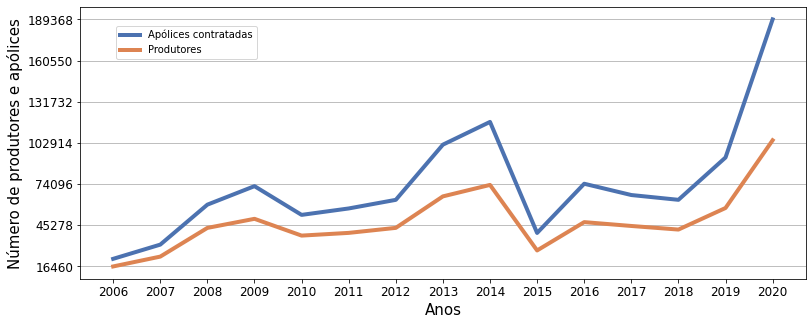
\includegraphics[width=0.8\textwidth]{figuras/apolices_produtores.png}\\
	%\small \textsuperscript {Fonte: Elaboração própria a partir de dados da Plataforma Atlas do Seguro Rural \cite{brasil21b}.}
    \parbox{\dimexpr\linewidth-3cm}{\raggedright
    \strut \textsuperscript{Fonte: Elaboração própria a partir de dados da Plataforma Atlas do Seguro Rural \cite{brasil21b}.}\strut}
    \label{apolices_produtores}
\end{figure}

É importante destacar que, no ano de $2021$, até o mês de junho, havia $66.928$ apólices contratadas \cite{brasil21}. Apesar do valor ser baixo se comparado ao ano de $2020$ ($189.368$ apólices), já é superior a $56,25\%$ dos anos anteriores. Padrão semelhante se observa com o número de produtores. No ano de $2021$, até o mês de junho haviam sido contabilizados $47.472$ produtores segurados \cite{brasil21b}.

%\subsubsection{Valores do prêmio e de subvenção ao prêmio de seguro rural}

O gráfico da Figura \ref{soma_ano_values} apresenta a evolução dos valores em milhões de reais de subvenção ao prêmio de seguro rural, prêmio pago pelo produtor e prêmio recebido pela seguradora entre $2006$ a $2020$. Observa-se que, com exceção do ano de $2014$, é possível notar uma tendência de crescimento dos valores de subvenção e prêmio pagos no período analisado. No ano de 2014, devido à contenções, o governo federal liberou apenas R\$ $400$ milhões dos R\$ $700$ milhões previstos para subsidiar o seguro rural. Esta contenção dos gastos governamentais pode ser um fator a ser considerado na queda dos valores do seguro rural ocorrida entre os anos de $2014$ e $2015$ \cite{andrade21}.

Em $2021$, até o mês de junho, o valor do prêmio pago à seguradora já havia alcançado R\$$1,25$ bilhões, o quarto maior valor registrado e cerca de $50,59\%$ maior que a média. O prêmio do produtor referente ao período de janeiro a junho de $2021$ já era equivalente a R$\$0,77$ bilhões, valor cerca de $69,67\%$ maior que a média do prêmio de responsabilidade do produtor. O valor concedido na forma de subvenção ao prêmio em $2021$ também é o quarto maior valor registrado, cerca de $25,96\%$ maior que a média dos valores de subvenção concedidos . Além disso, a partir do ano de $2016$, a parcela do prêmio sob responsabilidade do produtor passa a superar a parcela concedida pelo governo na forma de subvenção \cite{brasil21b}.

%\begin{figure}[H]
%	\centering
%	\caption{Valores do prêmio e de subvenção ao prêmio de seguro rural. Brasil $2006 - 2020$}
%	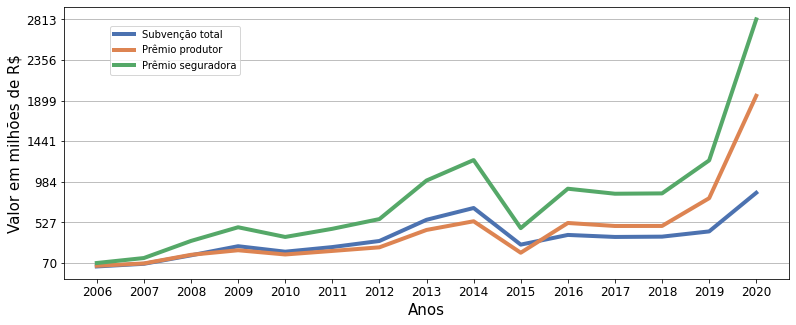
\includegraphics[width=0.8\textwidth]{figuras/soma_ano_values.png}\\
%	\small \textsuperscript {Fonte: Elaboração própria a partir de dados da Plataforma Atlas do Seguro Rural (Mapa, 2021).}
%    \label{soma_ano_values}
%\end{figure}

%\begin{figure}[H]
%	\centering
%	\caption{Soma da importância segurada (R\$ milhões). Brasil $2006 - 2020$}
%	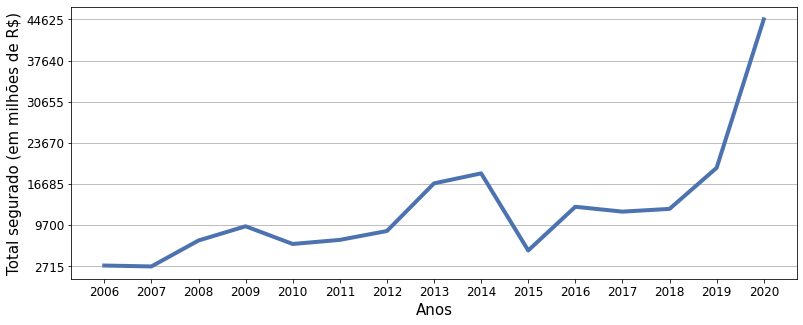
\includegraphics[width=0.8\textwidth]{figuras/total_segurado_mil.png}\\
%	\small \textsuperscript {Fonte: Elaboração própria a partir de dados da Plataforma Atlas do Seguro Rural (Mapa, 2021).}
%    \label{total_segurado_mil}
%\end{figure}

%\begin{figure}[H]
%	\centering
%	\caption{Total da área segurada em hectares. Brasil $2006 - 2020$}
%	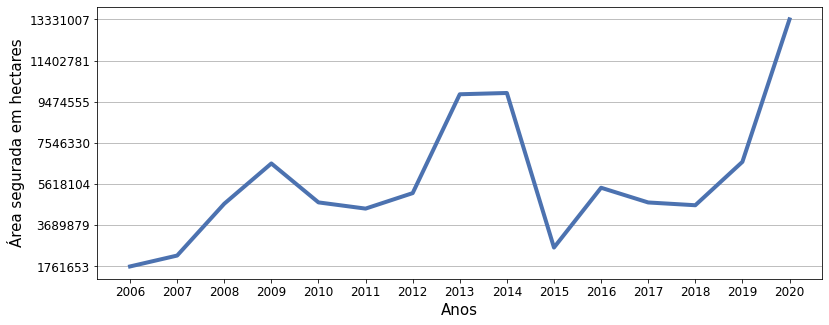
\includegraphics[width=0.8\textwidth]{figuras/area_segurada.png}\\
%	\small \textsuperscript {Fonte: Elaboração própria a partir de dados do Ministério da Agricultura, Pecuária e Abastecimento (MAPA).}
%    \label{area_segurada}
%\end{figure}

%\begin{figure}[H]
%	\centering
%	\caption{Número de apólices de seguro rural indenizadas. Brasil $2006 - 2019$}
%	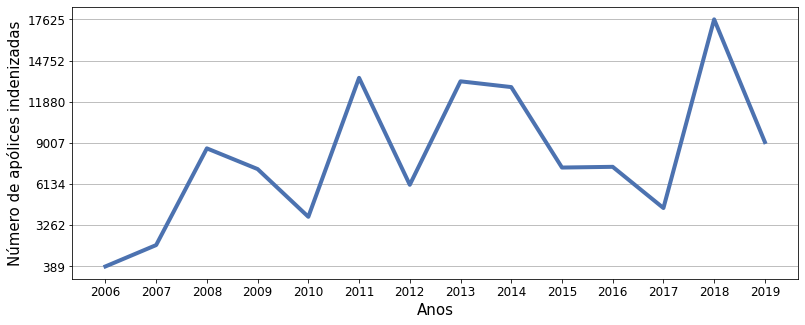
\includegraphics[width=0.8\textwidth]{figuras/apolices_indenizadas.png}\\
%	\small \textsuperscript {Fonte: Elaboração própria a partir de dados do Ministério da Agricultura, Pecuária e Abastecimento (MAPA)}
%    \label{apolices_indenizadas}
%\end{figure}

%\begin{figure}[H]
%	\centering
%	\caption{Valor das indenizações de seguro rural pagas (R\$ milhões). Brasil $2006 - 2019$}
%	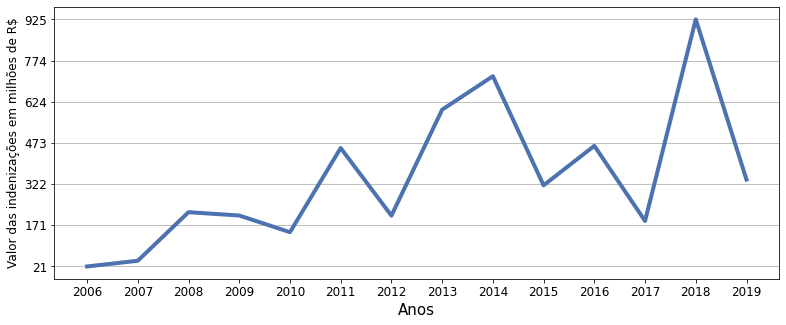
\includegraphics[width=0.8\textwidth]{figuras/valor_indenizacoes.png}\\
%	\small \textsuperscript {Fonte: Elaboração própria a partir de dados do Ministério da Agricultura, Pecuária e Abastecimento (MAPA)}
%    \label{valor_indenizacoes}
%\end{figure}

% variaveis_br
\begin{figure}[H]
	\centering
	\caption{Evolução das variáveis de seguro rural no Brasil}\label{variaveis_br}
	\small
	
	\subfloat[Valores do prêmio e de subvenção ao prêmio de seguro rural\label{soma_ano_values}]{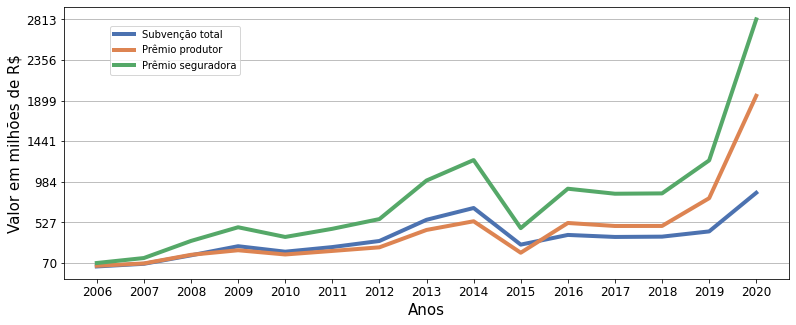
\includegraphics[width=0.45\textwidth]{figuras/soma_ano_values.png}}\hspace{0.1cm}
	\subfloat[Soma da importância segurada (R\$ milhões)\label{total_segurado_mil}]{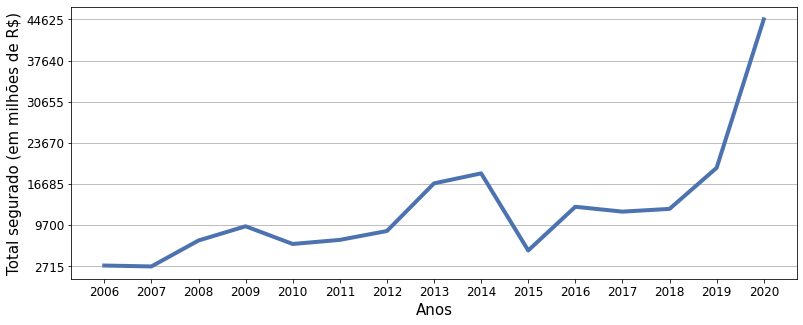
\includegraphics[width=0.45\textwidth]{figuras/total_segurado_mil.png}}\hspace{0.1cm}\\
	
	\subfloat[Total da área segurada em hectares.\label{area_segurada}]{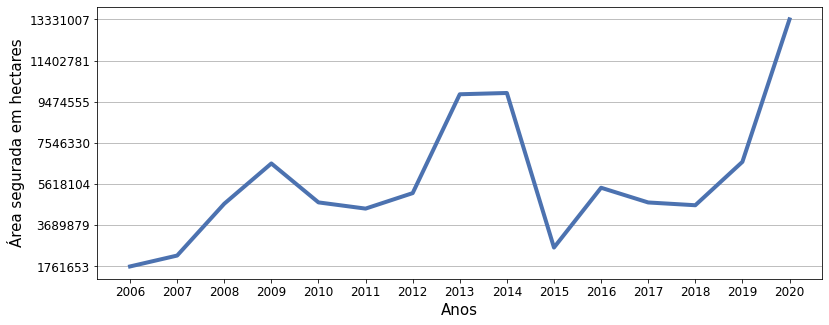
\includegraphics[width=0.45\textwidth]{figuras/area_segurada.png}}\hspace{0.1cm}
	\subfloat[Número de apólices de seguro rural indenizadas\label{apolices_indenizadas}]{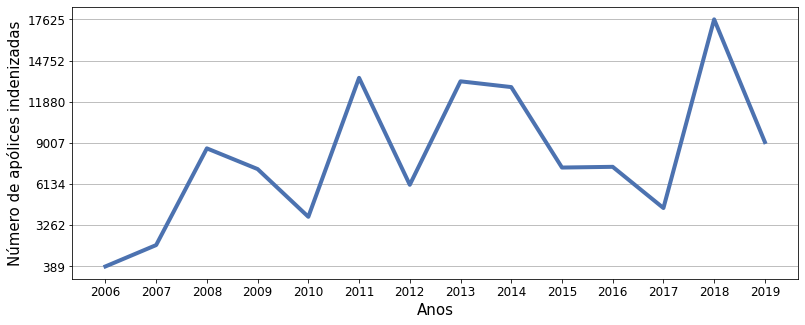
\includegraphics[width=0.45\textwidth]{figuras/apolices_indenizadas.png}}\\
	
	\subfloat[Valor das indenizações de seguro rural pagas (R\$ milhões)\label{valor_indenizacoes}]{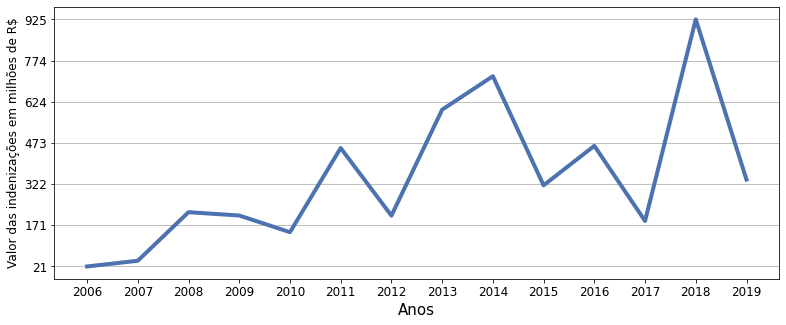
\includegraphics[width=0.45\textwidth]{figuras/valor_indenizacoes.png}}\hspace{0.1cm}
	\subfloat[Taxa média anual de contratação do prêmio de seguro rural\label{taxa_media}]{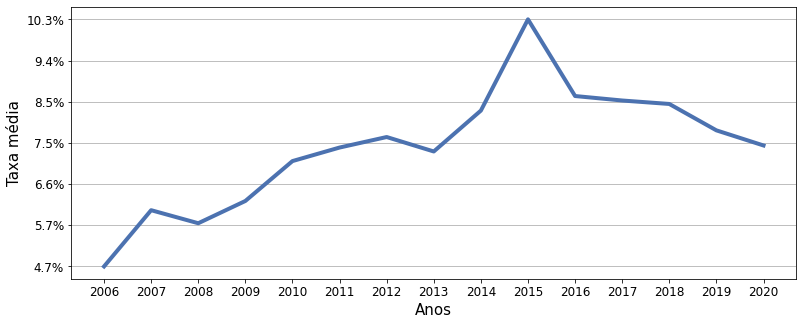
\includegraphics[width=0.45\textwidth]{figuras/taxa_media.png}}
	
	\parbox{\dimexpr\linewidth-2cm}{\raggedright
    \strut \textsuperscript{Fonte: Elaboração própria a partir de dados do Ministério da Agricultura, Pecuária e Abastecimento e da Plataforma
	Atlas do}\strut}\\
    \parbox{\dimexpr\linewidth-2cm}{\raggedright
    \strut \textsuperscript{Seguro Rural \cite{brasil21b}.}\strut}
\end{figure}

Os valores da soma da importância segurada em milhões de reais são apresentados no gráfico da Figura \ref{total_segurado_mil}. Observa-se que há crescimento dos valores segurados, com destaque para o crescimento entre os anos de $2019$ e $2020$, em que o os valores mais que duplicaram. Considerando o período entre $2006$ e $2020$, o crescimento da importância segurada foi de $15,55$ vezes o valor de $2006$. Também é possível observar que, entre os anos de $2014$ e $2015$, ocorreu uma queda de $70,68\%$ do valor segurado.  

Em $2020$, o Programa de Subvenção ao Prêmio do Seguro Rural (PSR) aplicou R\$ $880$ milhões, ou seja, o dobro do valor executado no ano de  $2019$. Para o ano de $2021$, a estimativa apresentada pelo Ministério da Agricultura e Abastecimento foi um aumento de R\$ $1$ bilhão a verba destinada ao PSR \cite{brasil21b}.

No ano de $2014$, o total segurado chegou a R$\$18.462,88$ milhões, no entanto, em $2015$ a soma da importância caiu para R$\$5.398,54$ milhões, o terceiro valor mais baixo do período. O valor mais alto ocorre no ano de $2020$, em que o valor segurado foi de R$\$45,7$ bilhões, o maior desde o início do programa em $2005$.

O valor da importância segurada alcançou $R\$14,4$ bilhões até o mês de junho de $2021$. Este valor é o quinto maior valor da série e já é maior que $25\%$ dos valores registrados nos anos anteriores \cite{brasil21b}. 

%\subsubsection{Área segurada em hectares}

A Figura \ref{area_segurada} apresenta o total da área segurada em hectares nos municípios do Brasil entre os anos de  $2006$ e  $2020$. É possível observar que, a área agrícola segurada no país praticamente dobrou entre $2019$ e $2020$, quando alcançou o maior valor, $13,7$ milhões de hectares, o que representou $20\%$ da área total agrícola do país. O aumento de área em relação a $2019$ é de $98\%$. O maior valor registrado em anos anteriores foi em $2014$, quando foram segurados $9,4$ milhões de hectares. No ano de $2021$, até o mês de junho, foram segurados cerca de $3,76$ milhões de hectares. Esse valor representa cerca de $71,76\%$ da área segurada em $2020$ \cite{brasil21b}. 

%\subsubsection{Indenizações}

Com relação ao número de indenizações,  o gráfico da Figura \ref{apolices_indenizadas} apresenta a evolução das apólices indenizadas ao longo do período analisado. O menor número de indenizações é $389$ em $2006$ e o maior valor ocorreu no ano de $2018$, sendo igual a $17.625$ indenizações. Durante o período, ocorre em média um número de $8.110$ apólices indenizadas por ano, sendo que o crescimento no número de apólices indenizadas foi de $23,31$ vezes entre $2006$ e $2019$. 

Os valores pagos como indenização entre os anos de $2006$ e $2019$ são apresentados no gráfico da Figura \ref{valor_indenizacoes} e variam entre R\$ $20.699.785,74$ em $2006$ e R\$ $924.988.210,45$ em $2018$. A média do valor das indenizações foi de R\$ $345.525.736,50$ no período analisado. 

%\begin{small}
%    \begin{table}[H]
%        \caption{Número de apólices de seguro rural indenizadas por regiões. Brasil $2006-2019$}\label{premio_regioes}
%         \input{../anexos/ap_indeniz_regioes.tex}
%    \end{table}
%\end{small}

%\subsubsection{Taxa média de contratação de seguro rural}

O gráfico apresentado na Figura \ref{taxa_media} mostra a trajetória da taxa de contratação do seguro rural. É possível constatar que a taxa se eleva, em média, de $4,7\%$ em $2006$ para $ 7,46\%$ em $2020$. Até o mês de junho de $2021$, o valor da taxa média havia alcançado $9,79\%$, o segundo maior valor da série, sendo superado pela taxa média cobrada em $2015$, que foi de $10,3\%$ \cite{brasil21b}.  

Segundo Santos e Silva (2017), espera-se que, à medida que o sistema de seguro rural se consolida, reduzam-se os preços das apólices devido aos ganhos de produtividade agropecuária e da redução de fatores de risco. Essas reduções podem ocorrer devido à adoção das orientações do zoneamento agrícola, de um maior conhecimento do histórico de eventos climáticos e dos sinistros ocorridos e, até mesmo em função da adoção de tecnologias, como o uso de irrigação etc. No entanto, essa redução das taxas não ocorreu no período analisado, como observado na Figura \ref{taxa_media}. 

%\begin{figure}[H]
%	\centering
%	\caption{Taxa média anual de contratação do prêmio de seguro rural. Brasil $2006 - 2020$}
%	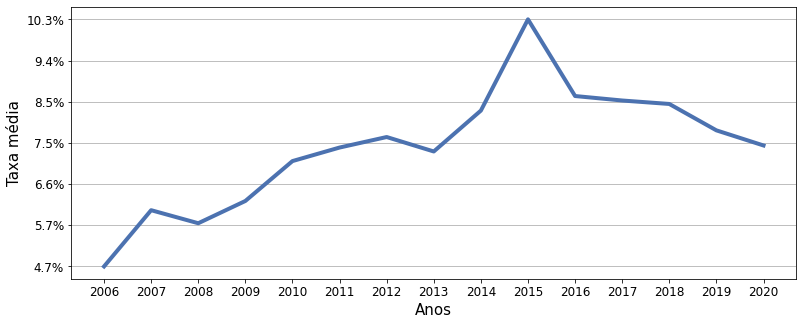
\includegraphics[width=0.8\textwidth]{figuras/taxa_media.png}\\
%	\small \textsuperscript {Fonte: Elaboração própria a partir de dados da Plataforma Atlas do Seguro Rural (Mapa, 2021).}
%   \label{taxa_media}
%\end{figure}

%\begin{small}
%\begin{table}[H]
%\caption{Taxa média de contratação do prêmio de seguro rural por regiões.  Brasil $2006-2020$}\label{tx_media_regioes}
% \input{../anexos/tx_media_regioes.tex}
%\end{table}
%\end{small}

%\subsubsection{Culturas}

A Figura \ref{percent_cult_apol} apresenta o percentual da participação das maiores culturas no número de apólices de seguro rural contratadas. A análise desse gráfico permite identificar que, com exceção de $2015$, a cultura da soja foi a que mais contratou seguro rural. Além disso, observa-se que o milho 2ª safra \footnote{Nesse caso o milho de 2ª safra é listado em separado devido aos distintos graus de risco em relação à 1ª safra \cite{santos17}.} tem cada vez mais aumentado sua participação no número de apólices contratadas. O milho 1ª safra, por sua vez, tem participação que varia entre $1,23\%$ e $16,46\%$, com média de  $6,16\%$ ao longo do período. A participação da cultura da maçã na contratação de seguro rural permanece relativamente estável ao longo do período, variando entre $8,79\%$ e $14,72\%$. 

\begin{figure}[H]
	\centering
	\caption{Percentual da participação das maiores culturas no número de apólices de seguro rural contratadas. Brasil $2006 - 2019$}
    	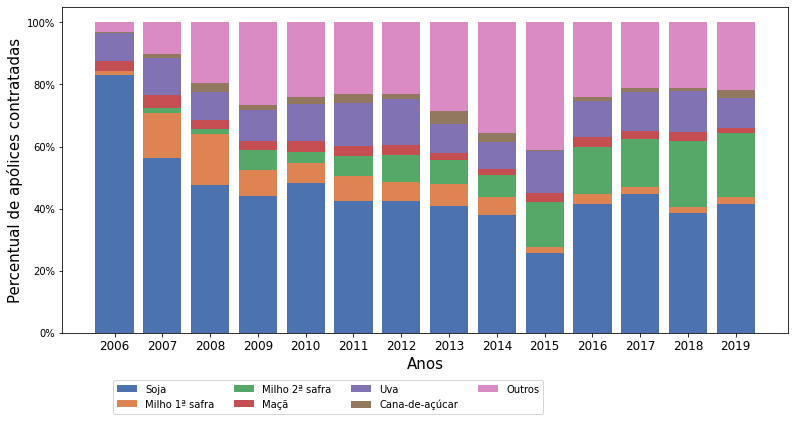
\includegraphics[width=0.8\textwidth]{figuras/percent_apolic_cult.png}\\
	%\small \textsuperscript {Fonte: Elaboração própria a partir de dados do Ministério da Agricultura, Pecuária e Abastecimento \cite{brasil21b}}
	\parbox{\dimexpr\linewidth-2.8cm}{\raggedright
    \strut \textsuperscript{Fonte: Elaboração própria a partir de dados do Ministério da Agricultura, Pecuária e Abastecimento \cite{brasil21b}.}\strut}
    \label{percent_cult_apol}
\end{figure}

A Tabela \ref{percent_culturas} apresenta a participação percentual de grupos de culturas em variáveis do seguro rural. É possível constatar que entre os anos de $2006$ e $2020$, as culturas de grãos foram responsáveis por $74,85\%$ das apólices contratadas, seguida das culturas de frutas com $14,74\%$ das apólices no período. Em terceiro lugar está a cultura de olerícolas, com cerca de $3,36\%$ de participação na contratação de apólices de seguro rural. Uma estrutura semelhante de participação percentual de grupos de culturas pode ser observada com relação à participação no valor total segurado. O grupo de cultura que mais se destaca é a dos grãos, com $74,88\%$ do total segurado, seguido das frutas e do café, com $9,55\%$ e $4,04\%$, respectivamente. 

\begin{small}
\begin{table}[H]
\caption{Participação percentual das culturas nos valores do seguro rural. Brasil $2006-2020$}\label{percent_culturas}
 \footnotesize
\vspace{0.05cm}
\begin{tabularx}{\textwidth}{lRRRRR}
    \hline \\[-1.9ex]	 
    Cultura    & \% das apólices & \% do total segurado & \% do premio total & \% de subvenção & Taxa média \\
    \hline \\[-1.9ex]	 
    Grãos      & 74,85\%         & 74,88\%              & 78,86\%            & 77,35\%         & 7,70\%     \\
    Frutas     & 14,74\%         & 9,55\%               & 13,14\%            & 16,07\%         & 9,17\%     \\
    Olerícolas & 3,36\%          & 2,74\%               & 3,17\%             & 2,85\%          & 7,64\%     \\
    Café       & 3,07\%          & 4,04\%               & 2,19\%             & 1,61\%          & 3,15\%     \\
    Cana       & 2,08\%          & 2,98\%               & 0,77\%             & 0,69\%          & 1,63\%     \\
    Pecuária   & 0,73\%          & 1,16\%               & 0,77\%             & 0,32\%          & 3,26\%     \\
    Floresta   & 0,30\%          & 3,51\%               & 0,42\%             & 0,35\%          & 1,60\%     \\
    Outros     & 0,88\%          & 1,13\%               & 0,68\%             & 0,75\%          & 4,64\%     \\ 
    \hline 
\end{tabularx}
%\vspace{0.5cm}
\small \textsuperscript{Fonte: Elaboração própria a partir de dados da Plataforma Atlas do Seguro Rural (Mapa, 2021).  }\\
\end{table}
\end{small}

Além disso, é possível observar na Tabela \ref{percent_culturas}, os percentuais de subvenção ao prêmio de seguro rural e os valores da taxa média de contratação do seguro. As taxas cobradas durante o período para a cultura de grãos foi de $7,70\%$, a taxa cobrada das culturas de frutas foi de $9,17\%$ e as olerícolas tiveram uma taxa média de contratação de $7,64\%$. Os percentuais de subvenção dessas culturas são, também, os mais altos: $77,35\%$ de subvenção para os grãos, $16,07\%$ para as culturas de frutas e $2,85\%$ para as olerícolas. Ou seja, os grupos de culturas com maior demanda pelo seguro, além de apresentarem os maiores valores de apólices, os maiores valores e maior ocorrência de sinistros, são também aqueles com maiores taxas médias. 

De acordo com  Santos e Silva (2017), este fato pode apontar para a possibilidade de dois fenômenos a serem melhor examinados. O primeiro diz respeito à situação em que as maiores taxas resultam do fato de que maiores subvenções são dadas a cultivos de maior risco. O segundo fenômeno possível é que as taxas sejam mais altas, principalmente no caso dos produtores que adotam o ZARC, com elevada tecnologia produtiva, alta produtividade e não têm estas características levadas em consideração como informação que contribui para a redução das taxas. Dessa forma, se por um lado o seguro agrícola não se consolida sem a subvenção dada pelo Estado, por outro, é possível que esse sistema de subvenção ao prêmio crie distorções no mercado de seguro rural. 

%\subsubsection{Seguradoras}

A Tabela \ref{seguradoras} exibe a distribuição das fatias de mercado das seguradoras entre $2006$ e $2020$. Apesar de as seguradoras passarem de cinco, em $2006$, para $16$ companhias aptas a operar com seguro rural em $2020$, é possível constatar que há uma concentração do mercado de seguro em um número reduzido de seguradoras. 

\begin{small}
\begin{table}[H]
\caption{Participação de mercado das seguradoras. Brasil $2006-2020$}\label{seguradoras}
 \footnotesize
\vspace{0.05cm}
\begin{tabularx}{\textwidth}{lRRRRRRR}
    \hline \\[-1.9ex]	 
    Seguradora         & Apólices        & \% do número de apólices  & Beneficiários  & \% dos beneficiários  & Área segurada (em mil ha)  & \% de área segurada   \\
    \hline \\[-1.9ex]	 
    Brasilseg         &  $410.892$      &  $37,23  $                &  $95.769$                    &  $26,85  $            &  $48.076,26$       & $55,31  $              \\
    Mapfre            &  $149.389$      &  $13,54  $                &  $49.274$                    &  $13,82  $            &  $7.309,17$        &  $8,41  $               \\
    Essor             &  $119.087$      &  $10,79  $                &  $38.995$                    &  $10,93  $            &  $4.603,47$        &  $5,30  $               \\
    Swiss Re          &  $91.410$       &  $8,28  $                 &  $34.483$                    &  $9,67  $             &  $7.870,31$        &  $9,06  $               \\
    Nobre             &  $82.500$       &  $7,48  $                 &  $29.053$                    &  $8,15  $             &  $2.747,88$        &  $3,16  $               \\
    Allianz           &  $66.983$       &  $6,07  $                 &  $21.210$                    &  $5,95  $             &  $5.387,98$        &  $6,20  $               \\
    Sancor            &  $49.567$       &  $4,49  $                 &  $22.516$                    &  $6,31  $             &  $3.210,37$        &  $3,69  $               \\
    Fairfax           &  $35.343$       &  $3,20  $                 &  $18.349$                    &  $5,14  $             &  $2.055,87$        &  $2,37  $               \\
    Porto Seguro      &  $26.306$       &  $2,38  $                 &  $6.152$                     &  $1,72  $             &  $259,33$          &  $0,30  $               \\
    Newe              &  $22.741$       &  $2,06  $                 &  $12.337$                    &  $3,46  $             &  $1.469,10$        &  $1,69  $               \\
    Tokio Marine      &  $19.808$       &  $1,79  $                 &  $11.263$                    &  $3,16  $             &  $1.722,64$        &  $1,98  $               \\
    Too               &  $14.844$       &  $1,35  $                 &  $9.768$                     &  $2,74  $             &  $1.163,48$        &  $1,34  $               \\
    Aliança do Brasil &  $7.200$        &  $0,65  $                 &  $3.294$                     &  $0,92  $             &  $593,19$          &  $0,68  $               \\
    Excelsior         &  $4.472$        &  $0,41  $                 &  $2.292$                     &  $0,64  $             &  $238,97$          &  $0,27  $               \\
    Sompo             &  $3.062$        &  $0,28  $                 &  $1.901$                     &  $0,53  $             &  $181,66$          &  $0,21  $               \\
    Itaú              &  $9$            &  $0,00  $                 &  $9$                         &  $0,00  $             &  $25,10$           &  $0,03  $               \\
    \hline \\[-1.9ex]
    \textbf{Total}    & \textbf{1.103.613} & \textbf{100  }         & \textbf{213.692}             & \textbf{100  }        & \textbf{86.914,79} & \textbf{100  }\\
	\hline 
\end{tabularx}
%\vspace{0.5cm}
\small \textsuperscript{Fonte: Elaboração própria a partir de dados da Plataforma Atlas do Seguro Rural (Mapa, 2021).}\\
\footnotesize{Nota: Valores acumulados $2006 -- 2020$}\\
\end{table}
\end{small}

Ao se analisar a participação no percentual do número de apólices de seguro rural, percebe-se que apenas as três maiores seguradoras (Brasilseg, Mapfre e Essor) concentram cerca de $61,56\%$ do mercado. Com relação ao percentual dos beneficiários, as três maiores seguradoras contam com cerca de $51,60\%$ dos beneficiários durante o período analisado. A concentração é ainda maior quando se analisa o percentual da área segurada, sendo que a  maior seguradora do ramo (Brasilseg) conta com um percentual de $55,31\%$ da área segurada em hectares. As três maiores seguradoras são responsáveis pelo seguro de $72,78\%$ da área segurada. 

%A próxima seção tem como objetivo apresentar os resultados da análise da distribuição espacial dos dados do seguro rural no Brasil. 

\subsection{A DISTRIBUIÇÃO REGIONAL DO SEGURO RURAL} 

Os gráficos apresentados na Figura \ref{variaveis_regioes} exibem a evolução, entre os anos de $2006$ e $2019$, das variáveis de seguro rural analisadas por regiões.

Na figura \ref{ap_contrat_regioes}, é possível observar a evolução do número de apólices contratadas nas regiões brasileiras. Na Figura \ref{ap_contrat_regioes}, observa-se que a região Sul se destaca das demais com relação ao número de apólices contratadas. O menor número de apólices contratadas na região Sul foi de $16.525$ apólices no ano de $2006$. O valor médio de apólices contratadas durante o período foi $44.166$ apólice. No ano de $2014$, foi registrado o maior número de apólices contratadas ($76.668$ apólices). 

% variaveis_regioes
\begin{figure}[H]
	\centering
	\caption{Evolução das variáveis de seguro rural por regiões. Brasil $2006 - 2019$}\label{variaveis_regioes}
	\small
	
	\subfloat[Número de apólices contratadas\label{ap_contrat_regioes}]{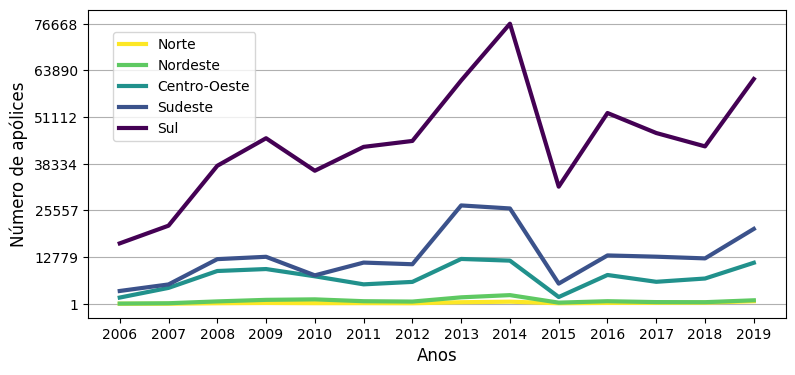
\includegraphics[width=0.45\textwidth]{figuras/ap_contrat_regioes.png}}\hspace{0.1cm}
	\subfloat[Total segurado (em milhões de R\$)\label{t_segurado_regioes}]{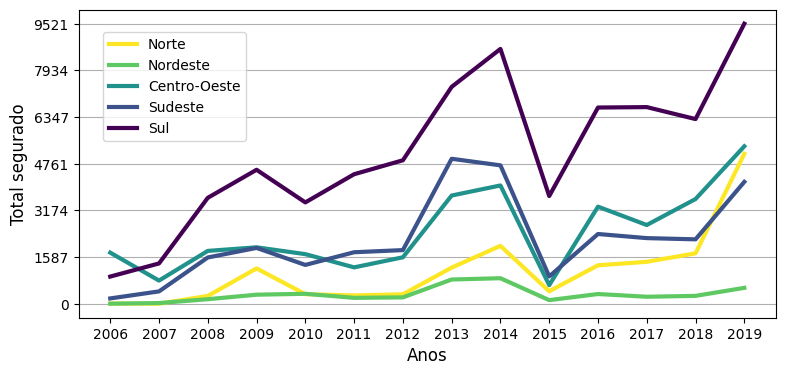
\includegraphics[width=0.45\textwidth]{figuras/t_segurado_regioes.png}}\\
	
	\subfloat[Valores de prêmio (em milhões de R\$)\label{soma_premio_regioes}]{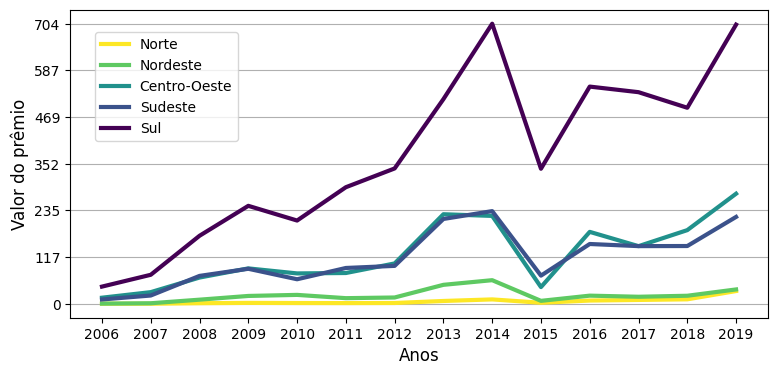
\includegraphics[width=0.45\textwidth]{figuras/soma_premio_regioes.png}}\hspace{0.1cm}
	\subfloat[Valores subvenção (em milhões de R\$)\label{t_subvencao_regioes}]{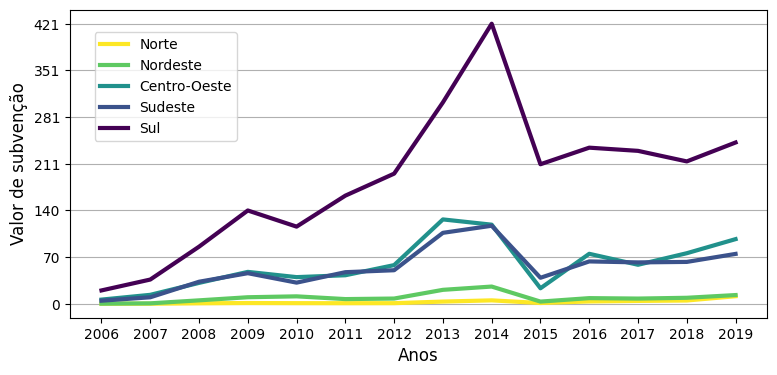
\includegraphics[width=0.45\textwidth]{figuras/t_subvencao_regioes.png}}\\
	
	\subfloat[Apólices indenizadas\label{ap_indeniz_regioes}]{\includegraphics[width=0.45\textwidth]{figuras/ap_indeniz_regioes.png}}\hspace{0.1cm}
	\subfloat[Valor das indenizações (em milhões de R\$)\label{inde_pagas_regioes}]{\includegraphics[width=0.45\textwidth]{figuras/inde_pagas_regioes.png}}\\
	
    \parbox{\dimexpr\linewidth-2cm}{\raggedright
    \strut \textsuperscript{Fonte: Elaboração própria a partir de dados do Ministério da Agricultura, Pecuária e Abastecimento \cite{brasil21b}}\strut}
\end{figure}

A segunda região com maior número de apólices contratadas é a região Sudeste (Figura \ref{ap_contrat_regioes}). Em média, na região Sudeste, foram contratadas $12.942$ apólices por ano, o maior valor registrado foi $26.913$ apólices contratadas em $2013$. A região Centro-Oeste é a terceira região com mais apólices contratadas, sendo que em média foram contratadas $7.225$  por ano e, em $2013$ foi registrado o maior número de apólices ($12.260$). Por fim, as regiões Norte e Nordeste, apresentaram respectivamente, em média, $240$ e $804$ apólices contratadas por ano.

A taxa de crescimento do número de apólices contratadas na região sul foi de $3,72$ vezes o valor inicial entre os anos $2006$ e $2019$. Por sua vez, durante o período analisado a região Sudeste teve um crescimento do número apólices de $5,87$ vezes e a região Centro-Oeste apresentou um crescimento do número de apólices de $6,66$ vezes. As regiões Norte e Nordeste apresentaram um crescimento médio anual igual a $0,14\%$ e $4,04\%$ respectivamente. 

Ao se analisar a evolução do total segurado nas regiões brasileiras apresentado na Figura \ref{t_segurado_regioes}, é possível observar que a região Sul se destaca com, em média, $5146,83$ milhões de valor segurado total. O maior valor foi registrado em $2019$ e foi igual a $9520,85$ milhões, o segundo maior valor foi igual a $8664,31$ milhões e foi registrado em $2015$. 

No início da série valores a região Centro-Oeste apresenta um maior valor total segurado do que a região Sul (5.355 milhões). Além disso, como é possível observar na Figura \ref{t_segurado_regioes}, a partir do ano de $2016$ a região Centro-Oeste supera a região Sudeste no valor total segurado. A região Norte apresentou, com relação ao total segurado, os valores de $120,35$ milhões em $2009$ e $197,01$ milhões em $2014$. 
Além disso, a região Norte apresenta o seu maior valor no ano de $2019$, com total segurado igual a $509,94$ milhões. Também é possível observar que há indícios de haver um crescimento do total segurado em todas as regiões. 

O total segurado na região Sul apresenta um crescimento de cerca de $10,27$ vezes entre os anos de $2006$ e $2019$. Na região Sudeste, o crescimento foi de $22,52$ vezes o valor registrado em $2006$. Por sua vez, o Centro-Oeste apresentou um crescimento de cerca de $3,07$ vezes o valor do total segurado durante o período. O valor do total segurado na região Norte cresceu $499.51$ vezes entre os anos $2006$ e $2019$. Por fim, no Nordeste, o valor total segurado apresentou um crescimento de $106,95$ vezes o valor inicial. 

Para mais, ao se analisar a Figura \ref{soma_premio_regioes} e \ref{t_subvencao_regioes}, é possível observar que as variáveis valores de prêmio e valores subvenção apresentam crescimento durante o período analisado. Também é possível observar que, com exceção das variáveis relacionadas à indenização, as variáveis apresentam uma queda entre os anos de $2014$ e $2015$.

É possível observar na Figura \ref{ap_indeniz_regioes}, que a região Sul se destaca quando se analisa o número de apólices indenizadas. Os valores variam de $237$ em $2006$ e $13812$ apólices indenizadas em $2019$. Em média, a região Sul teve cerca de $6364$ apólices indenizadas durante o período. Além disso, durante os anos analisados, houve um crescimento de $58,28\%$ no número de apólices de seguro rural indenizadas. A região Sudeste é a segunda região com maior número de apólices indenizadas, sendo que o menor número de apólices indenizadas na região Sudeste foi de $135$ e ocorreu em $2006$, com maior valor registrado em $2013$, equivalente a $2.616$. 

Ao longo dos anos analisados, a diferença entre o número de apólices na região Sul e Sudeste foi em média igual a $5.283$ apólices. A região Centro-Oeste foi responsável por, em média, $559,64$ apólices indenizadas. O maior número de apólices indenizadas na região Centro-Oeste foi registrado em $2018$ e foi igual a $1561$ apólices. As regiões Norte e Nordeste tiveram em média $15,57$ e $88,64$, respectivamente. 

Com relação ao valor das indenizações de seguro rural pagas, é possível observar na Figura \ref{inde_pagas_regioes}, que a região Sul é a que possui os maiores valores pagos como indenização. Em média, foram pagos R$\$205,66$ milhões como indenização. O maior valor foi equivalente a R$\$551,74$ milhões e foi registrado em $2018$ e o menor valor foi registrado no primeiro ano analisado, sendo equivalente a R$\$15.06$ milhões. 

A Tabela \ref{media_regioes} apresenta a média dos valores anuais das variáveis de seguro rural acumulados por regiões no Brasil no período de $2006$ e $2019$. Como é possível observar, que a região Sul se destaca das demais com os maiores valores das médias das variáveis. Com relação ao número de apólices contratadas, a segunda região com maior média da variável total de apólices contratadas é o Sudeste. No entanto, quando se analisa a média da soma da importância seguradas, a segunda região com maior média é a região Centro-Oeste. A região Centro-Oeste, também conta com maiores médias nas variáveis soma dos prêmios pagos, total da subvenção e soma das indenizações pagas com relação às regiões Norte, Nordeste e Sudeste. A região Sudeste apresenta a maior média anual do número de apólices indenizadas. 



\begin{small}
\begin{table}[H]
\caption{Média anual dos valores das variáveis de seguro rural por regiões. Brasil $2006-2019$}\label{media_regioes}
\begin{center}
\footnotesize
    \begin{tabular}{lrrrrr}
    \hline \\[-1.9ex]	
    Variável                                  & Norte   & Nordeste & Centro-Oeste & Sudeste  & Sul       \\
    \hline \\[-1.9ex]	
    Total de apólices contratada              &  240,14 &   803,57 &      7.225,36 &  12.941,5 &  44.166,14 \\
    Soma da importância segurada (R\$ milhão) &   111,5 &   319,82 &      2.428,79 &  2.178,54 &   5.146,84 \\
    Soma dos prêmios (R\$ milhão)             &    6,37 &    20,76 &       123,43 &   115,02 &    371,72 \\
    Total de subvenção (R\$ milhão)           &    2,66 &     9,25 &        58,25 &    53,52 &    186,56 \\
    Soma das indenizações pagas (R\$ milhão)  &    2,39 &    18,73 &        68,59 &    50,15 &    205,66 \\
    Taxa média aplicada às apólices           &    0,01 &     0,01 &         0,13 &     0,11 &      0,45 \\
    Número de apólices indenizadas            &   15,57 &    88,64 &       559,64 &  1.081,57 &   6.364,57 \\
    \hline 
    \end{tabular}
\end{center}
\small \textsuperscript {Fonte: Elaboração própria a partir de dados do Ministério da Agricultura, Pecuária e Abastecimento (MAPA)}\\


\end{table}
\end{small}

A média dos valores anuais da taxa média de contratação de apólices indica que, a região Sul é a que possui maior taxa de contratação de seguro com taxa média igual a $0,45$ ao longo dos anos. A região Centro-Oeste é a que tem o segundo maior valor de taxa média durante os anos, sendo igual a $0,13$. As regiões Norte e Nordeste apresentaram taxa média igual a $0,01$.

\subsection{DISTRIBUIÇÃO ESPACIAL DO SEGURO RURAL}

A análise da distribuição espacial das variáveis se inicia com a visualização dos mapas temáticos. Por meio destes mapas, busca-se identificar visualmente se há a ocorrência de padrões na distribuição espacial das variáveis do seguro rural.

O primeiro grupo de mapas, apresentado na Figura \ref{map_segurado}, exibe a distribuição espacial da soma da importância segurada (R\$ milhão) nos municípios brasileiros entre os anos de $2006$ e $2019$. Para a construção dos mapas, os valores da variável foram divididos em 5 intervalos \footnote{Para a criação dos intervalos foi aplicado algoritmo Fisher Jenks aos valores das variáveis diferentes de $0$ e os intervalos foram criados tendo como referência os valores do ano de 2019 \cite{jenks77}}.

\begin{figure}[H]
	\centering
	\caption{Total segurado por municípios (em mil R\$). Brasil $2006 - 2019$}
	\includegraphics[width=0.9\textwidth]{figuras/map_total_segurado_mil.png}
	\small \textsuperscript {Fonte: Elaboração própria a partir de dados do Ministério da Agricultura, Pecuária e Abastecimento \cite{brasil21b}}
    \label{map_segurado}
\end{figure}

Pela análise da Figura \ref{map_segurado}, é possível observar que a distribuição espacial do total segurado se modificou no decorrer dos anos, apesar de se concentrar principalmente nas Regiões Sul e Centro-Oeste. É possível também destacar que, durante o período analisado, há indícios de concentrações espaciais na região do Extremo Oeste Baiano no Estado da Bahia, Sudoeste de Mato Grosso do Sul, Sul Goiano no Estado de Goiás e Sudeste, no sul do Estado de São Paulo.

O conjunto de mapas apresentado na Figura \ref{map_apolices}, exibe o número de apólices de seguro rural contratadas por municípios entre $2006$ e $2019$. Ao longo dos anos, o número de municípios com nenhuma apólice contratada cai e há indícios de um aumento do número de apólices até o ano de $2014$. Entre os anos de $2014$ e $2015$, há uma queda no número de apólices contratadas, como já foi mostrado no gráfico da Figura \ref{apolices_produtores}, e das demais variáveis relacionadas ao seguro rural. Essa redução também pode ser visualizada no mapa da Figura \ref{map_apolices}, em que o ano de $2015$ apresenta municípios com menor número de apólices contratadas. 

Ao se analisar a distribuição espacial, observa-se que há indícios de haver uma maior concentração espacial do total segurado e do número de apólices de seguro rural contratadas em algumas regiões. A partir do ano de $2015$ a retomada do crescimento destas variáveis (Figura \ref{total_segurado_mil}) pode ser visualizado com um maior número de áreas de coloração mais escura nos mapas (Figuras \ref{map_segurado} e \ref{map_apolices}).

\begin{figure}[H]
	\centering
	\caption{Número de apólices de seguro rural contratadas por municípios. Brasil $2006 - 2019$}
	\includegraphics[width=0.9\textwidth]{figuras/map_apolices_contratadas.png}
	\small \textsuperscript {Fonte: Elaboração própria a partir de dados do Ministério da Agricultura, Pecuária e Abastecimento \cite{brasil21b}}
    \label{map_apolices}
\end{figure}

A distribuição espacial das demais variáveis analisadas apresenta um padrão semelhante ao observado com a soma da importância segurada (R\$ milhão)  \footnote{Os mapas da distribuição espacial das variáveis do seguro rural no Brasil são apresentados no apêndice A}. Dessa forma, os resultados corroboram a hipótese apresentada por Silva, Teixeira e Santos (2014) na investigação sobre a participação do PSR na universalização do acesso ao seguro rural. Ou seja, apesar da evolução do seguro rural em âmbito nacional, quando se observa a distribuição espacial, verifica-se que há, ao longo do tempo, uma concentração das apólices e subvenções na região Sul e Centro-Oeste. Portanto, apesar de ter ocorrido uma ampliação do seguro rural, esta ampliação ocorreu de forma concentrada, o que evidencia o cumprimento de forma parcial dos objetivos do PSR \cite{silva14}.

\section{CONSIDERAÇÕES FINAIS}

%O objetivo do presente trabalho foi analisar a evolução e a dinâmica espacial de variáveis do seguro rural nos municípios brasileiros entre 2006 e 2019. Além disso, buscou-se investigar a presença de padrões de distribuição espacial. A

A análise possibilitou constatar resultados positivos na evolução do seguro rural no Brasil. O número de apólices contratadas tem um crescimento de cerca de $8,69$ vezes seu valor inicial durante o período. Ademais, a área agrícola segurada no país praticamente dobrou entre os anos de $2019$ e $2020$, quando alcançou o maior valor, $13,7$ milhões de hectares, que representa $20\%$ da área total agrícola do país. 

Em geral, identificou-se que as maiores concentrações de apólices de seguro rural estão situadas nas regiões Sul, Centro-Oeste e Sudeste, no sul do Estado de São Paulo.  Para mais, ressalta-se que, embora mantenham a concentração do número de apólices contratadas, número de apólices indenizadas, valores de subvenção, indenização e prêmio, atualmente há expansão da demanda por seguros agrícolas. 

Apesar de os dados indicarem uma concentração geográfica da adesão ao sistema de seguro rural no Brasil, é necessário levar em consideração outros sistemas, como o Proagro e o programa Garantia Safra. É necessário, ainda, ressaltar que a adesão dos produtores deve ocorrer como uma resposta à percepção do risco das atividades agropecuárias, ou seja, o seguro deve difundir-se com base na compreensão dos riscos e das vantagens de sua contratação. 

Por fim, este trabalho pode ser entendido como uma abordagem inicial, a partir da qual é possível se introduzir novos métodos estatísticos a fim de aprimorar os resultados. Dentre esses métodos, destaca-se a Análise de Componentes Principais (ACP), que pode ser utilizada para reduzir o número de variáveis,  de forma a possibilitar a incorporação de informação de mais de uma variável na análise exploratória espacial.

\newpage
\addcontentsline{toc}{section}{\hspace*{\distnumber}REFERÊNCIAS}
\begin{center}
\section*{REFERÊNCIAS} 
\end{center}




% Use isso descomentado durante edição.
% Quando concluir a Tese, comente isso e use
% o código do bloco abaixo.
%\begin{singlespace}
%\renewcommand\refname{}
%\begin{flushleft}
%\bibliography{../tese/bibtese2}
%\end{flushleft}
%\end{singlespace}

%% Em cap1intriduc-corrigido.bbl foi feita correção manual de
%% algumas referências como por exemplo as citações
%% de Dissertação e Tese.
%% Então deixa-se de usar o arquivo cap1introduc.bbl gerado
%% automaticamente pelo abntcite, mas isso é só ao final.
\begin{singlespace}
\begin{flushleft}
\renewcommand\refname{}
\vspace*{-1.5cm}
\documentclass[10pt]{article}
%==========================================================================================

\usepackage[utf8]{inputenc}
\usepackage[brazil]{babel}
\usepackage[T1]{fontenc}
\usepackage{amsmath}
\usepackage{amsfonts}
\usepackage{mathrsfs}
\usepackage{amssymb}
\usepackage{graphicx}
\usepackage{geometry, calc, color, setspace}
\usepackage{indentfirst}
\usepackage{wrapfig}
\usepackage{boxedminipage}
\usepackage{enumerate}
\usepackage{float}
\usepackage{paralist}
\usepackage{comment}
\usepackage{icomma}
\usepackage{rotating}
\usepackage{multirow}
\usepackage[position=bottom]{subfig}
\usepackage{array}
\usepackage{tabularx}
\usepackage{float}
\usepackage{array}

\newcolumntype{L}[1]{>{\raggedright\let\newline\\\arraybackslash\hspace{0pt}}m{#1}}
\newcolumntype{C}[1]{>{\centering\let\newline\\\arraybackslash\hspace{0pt}}m{#1}}
%\newcolumntype{R}[1]{>{\raggedleft\let\newline\\\arraybackslash\hspace{0pt}}m{#1}}
\newcolumntype{R}{>{\raggedleft\let\newline\\\arraybackslash\hspace{0pt}}X}

\usepackage[alf,bibjustif]{abntex2cite}
%\usepackage{abntcite}

% Para o alinhamento dos títulos das figuras
\usepackage{caption}
%\captionsetup[figure]{format=hang,labelsep=endash,font=small,justification=RaggedRight,singlelinecheck=off, margin=1cm}
\captionsetup[subfigure]{textfont=small,singlelinecheck=off,justification=raggedright}


%%  Inserindo os códigos Python ==================================
\usepackage{listings}

%\definecolor{light_gray}{rgb}{0.97,0.97,0.97}
%\definecolor{mymauve}{rgb}{0.58,0,0.82}
%\definecolor{mygreen}{rgb}{0,0.6,0}

\lstset{
  language = Python,
  inputencoding = utf8,
  backgroundcolor = \color{white},
  columns=fullflexible,
  basicstyle=\ttfamily,
  breaklines=true,
  postbreak=\raisebox{0ex}[0ex][0ex]{\color{black}$\hookrightarrow$\space},
  keywordstyle=\color{black},      % keyword style
  stringstyle=\color{black},
  commentstyle=\color{black}
}

\newcommand{\HRule}{\noindent\rule{\linewidth}{0.2mm}}

\usepackage{mathpazo}                         % tem suporte matemático
\usepackage[scaled=0.85]{beramono}            % usa esta nos verbatins [scaled=0.9]

\renewcommand\UrlFont{\color{black}\rmfamily} 

\def\distnumber{2.3em}

%==========================================================================================

\author{Walef Machado de Mendonça\footnote{Mestrando em Estatística Aplicada e Biometria na Universidade Federal de Alfenas}\\
Patrícia de Siqueira Ramos\footnote{Professora da Universidade Federal de Alfenas, campus Varginha}}

%==========================================================================================


\title{O seguro rural no Brasil: evolução e distribuição espacial}

\date{}

\begin{document}

\maketitle

\begin{abstract}
As atividades agropecuárias se inserem em um contexto de adversidades que as colocam em situação diferenciada em relação aos riscos enfrentados pelos produtores. Tais atividades demandam grandes investimentos, o que faz com que sua atratividade esteja relacionada às formas existentes de gerenciamento de riscos. Uma das formas mais usuais de gerenciamento de risco neste setor é a contratação de Seguro Rural, uma vez que esta modalidade de seguro possibilita a recuperação da capacidade financeira do produtor na ocorrência de sinistros. Nesse sentido, o objetivo do trabalho é avaliar a distribuição e a dinâmica espacial de variáveis relacionadas às apólices de Seguro Rural contratadas nos municípios brasileiros no período de 2006 a 2019. Além disso, busca-se investigar a existência de dependência espacial e a presença de agrupamentos com grande número de apólices de Seguro Rural. Para tanto, utiliza-se os dados dos Censos do Seguro Rural, compilados pelo Ministério da Agricultura, Pecuária e Abastecimento (MAPA) e Análise Exploratória de Dados Espaciais (AEDE). Os resultados apontam que as maiores concentrações de apólices de Seguro Rural estão situadas nas regiões Sul e Centro-Oeste. Além disso, apesar de haver um aumento nas contratações de Seguro Rural, há também uma tendência de maior concentração espacial das apólices ao longo do período analisado. \\
\newline
\noindent {\textbf{Palavras-chave}}: Seguro rural. Política agrícola. Estatística espacial. Autocorrelação espacial. I de Moran.
\end{abstract}

\section{INTRODUÇÃO}

O setor agropecuário brasileiro tem se destacado nas últimas décadas por seu crescimento proveniente da aplicação de novas tecnologias ao clima tropical e a incorporação de novas áreas de terras \cite{brasil19a}. Segundo dados dos censos agropecuários, entre $2006$ e $2017$, tanto a área total quanto a produção agrícola e pecuária vivenciaram crescimento. Neste período houve um acréscimo de cerca de $5,8\%$ na área total dos estabelecimentos agropecuários \cite{ibge19}. Com relação à sua participação no PIB, em 2019, a parcela do agronegócio brasileiro foi de  $20,5\%$  do PIB nacional. Já em 2020, o setor agropecuário brasileiro alcançou a participação de $26,6\%$ do PIB. Em valores monetários, o PIB do País totalizou R\$ $7,45$ trilhões em 2020, e a participação do agronegócio chegou a quase R\$ $2$ trilhões \cite{cepea21}. 

Dada a relevância do setor agropecuário na economia brasileira, é necessário destacar que este ramo apresenta características muito específicas com relação à magnitude dos riscos aos quais está sujeito \cite{burgo05}. Alguns riscos mais relevantes se devem, principalmente, às instabilidades climáticas e ameaças sanitárias, que podem afetar a produção, ou à razões de mercado, como variações das taxas de câmbio e juros, ou a condições ligadas ao ambiente de negócios, tais como, alterações em marcos regulatórios e em políticas públicas. Todos esses fatores geram variações na renda do setor, que devem ser enfrentadas por meio de políticas de apoio à gestão de riscos \cite{brasil21}. 

Uma gestão de riscos apropriada tem potencial de afetar de forma positiva a estabilidade da renda do produtor e sua própria permanência no setor agropecuário. O gerenciamento de riscos agropecuários pode ocorrer de diversas maneiras, no entanto, a contratação de seguro é uma das medidas mais comuns. O seguro rural é uma importante ferramenta de mitigação de riscos e proteção da renda. Esta modalidade de seguro atua no sentido de amenizar as perdas e possibilitar a recuperação da capacidade financeira do produtor rural em caso de ocorrência de sinistros \cite{brasil19b}. 

Nesse sentido, o presente trabalho tem por objetivo, avaliar a distribuição espacial do seguro rural nos municípios brasileiros entre 2006 e 2019. Para tanto, busca-se investigar se, no Brasil, as variáveis de seguro rural se distribuem de forma aleatória no espaço ou se há padrões de distribuição espacial. Além disso, através da análise da distribuição espacial do seguro rural no período, busca-se identificar se há regiões que tiveram alterações significativas no número de contratações de seguro. Por fim, este estudo busca fornecer informações para o debate de aperfeiçoamentos no sistema de seguro rural brasileiro, de forma a contribuir para uma agricultura mais eficiente e com menores riscos para o produtor rural.

O trabalho está estruturado da seguinte forma: a próxima seção apresenta uma breve revisão de literatura sobre o seguro rural. A terceira seção apresenta os dados, os procedimentos de análise e recursos computacionais que serão utilizados. A quarta seção apresenta resultados e discussões. A última seção apresenta as considerações finais.

\section{UM PANORAMA DO SEGURO RURAL NO BRASIL}

No Brasil, as primeiras iniciativas de se instalar um sistema de seguro rural remontam à meados da década de $1930$ e desenvolveram-se principalmente nas esferas estaduais. Em $1939$, o Estado de São Paulo determinou a criação de um seguro obrigatório contra o granizo na produção de algodão \cite{maia11}. Segundo Silva, Teixeira e Santos (2014), os resultados do seguro para a proteção da lavoura algodoeira em São Paulo influenciaram a criação de novos programas como a Carteira de Seguro Agrícola contra Granizo para a Viticultura, criada em $1948$, e a Carteira de Seguro Agrícola contra Geada para Horticultura instituída em $1964$.

Além disso, Silva, Teixeira e Santos (2014) apontam em seu trabalho o seguro para granizo que foi criado no final da década de $1940$ no Instituto Rio-Grandense do Arroz (Irga), e o seguro criado pela Associação dos Fumicultores do Brasil (Afubra), que objetivava ressarcir com recursos próprios os produtores de fumo nos estados de Santa Catarina e Rio Grande do Sul.

Já no âmbito nacional, foi criado em $1948$, o Instituto de  Resseguros do Brasil (IRB), com o objetivo de reduzir os prejuízos de eventos adversos e assegurar uma maior estabilidade aos produtores rurais \cite{silva14}. Além disso, o Governo Federal criou, em $1954$, a Companhia Nacional de Seguro Agrícola (CNSA) e o Fundo de Estabilidade do Seguro Agrário. Para mais, Maia,  Roitman e de Conti (2011) evidenciaram que a estruturação e gestão dos seguros da CNSA ficaram, de início, sob responsabilidade do IRB. No entanto, segundo Gemignani (2000), as atividades da CNSA se encerraram em $1996$, em decorrência do insucesso em disseminar a adesão ao seguro rural de forma a possibilitar sua viabilidade econômica \cite{maia11, silva14}.

Na segunda metade da década de $1960$, são instituídos o Decreto-Lei nº $73$ ($1966$) e o Decreto nº $60.459$ ($1967$), que instituem os fundamentos institucionais para as atividades de seguro e a criação do Sistema Nacional de Seguros Privados (SNSP). O decreto de $1967$ também criou o Fundo de Estabilidade do Seguro Rural (FESR), cujos recursos inicialmente eram geridos pelo IRB e cujo objetivo principal era garantir a equilíbrio do sistema de seguro rural e fornecer uma cobertura adicional para os riscos de sinistro \cite{silva14}

% Até aqui Ok
Instituída em $1970$, a Resolução nº $5$ do Conselho Nacional de Seguros Privados teve uma função relevante na caracterização das modalidades de seguros agrários. Nesta Resolução, foi definido o seguro agrícola, que fornece cobertura contra perdas decorrentes de fenômenos meteorológicos, doenças e pragas, o seguro pecuário que fornece cobertura para morte de animais causadas por doenças ou acidentes, assim como, o seguro de benfeitorias e produtos agropecuários. Em suma, a Resolução nº $5$ também estabelece o seguro de crédito, que cobre incapacidade de pagamento de compradores dos produtos agropecuários \cite{silva14}.

A criação do Programa de Garantia da Atividade Agropecuária (Proagro), através da Lei nº $5.969$, de $11$ de dezembro de $1973$ ocorreu devido ao fato de que, apesar das diversas ações do Governo Federal, o seguro rural se desenvolveu de forma lenta e restrita à uma pequena parcela da produção \cite{silva14}. O Proagro inicialmente ficou sob a responsabilidade do Banco Central e passou a vincular o seguro rural às operações de crédito agropecuário. Por sua vez, o Banco Central utilizou emissões monetárias para pagamentos de sinistros. Segundo Maia, Roitman e De Conti (2011), o sistema de financiamento do Proagro gerou déficits que provocaram diversas alterações no Programa, que ainda permanece um dos mais importantes instrumentos para a gestão de riscos na agricultura no Brasil.

Instituído por meio da Lei nº $10.823$ de $19$ de dezembro de $2003$ e do Decreto nº $5.121$ de $2004$, o Programa de Subvenção ao Prêmio do Seguro Rural (PSR), passou a ser a política adotada pelo Governo Federal para o estímulo ao sistema de seguro rural no Brasil \cite{brasil18}. O PSR busca, assim como ocorre em países europeus e nos Estados Unidos, conceder subvenção econômica ao valor do prêmio do seguro rural contratado com seguradoras autorizadas \cite{maia11, silva14}.

Dessa forma, o PSR tem como finalidade subsidiar parte do prêmio do seguro rural, de modo a assegurar a responsabilidade do seguro rural como forma de garantir a estabilidade da renda do produtor, além de suscitar o aplicação das tecnologias adequadas para os empreendimentos agropecuários \cite{guia_20}. Tal política do governo busca tornar o seguro rural mais acessível aos agricultores, dividindo os custos de aquisição da apólice entre o governo e os produtores. 


\section{MATERIAL E MÉTODOS}\label{material_e_metodos}

%O objetivo dessa seção é apresentar os dados utilizados no trabalho, descrever a metodologia e os recursos computacionais utilizados na presente análise.

\subsection{DADOS}

% Fonte dos Dados 

Os dados de seguro rural utilizados neste trabalho foram obtidos no endereço eletrônico do Ministério da Agricultura, Pecuária e Abastecimento (MAPA) \cite{brasil21}. Foram utilizados dados com valores anuais a partir do ano de $2006$ até o ano de $2019$ (último ano disponível até então) para os dados municipais. Os dados agregados são provenientes do Atlas do Seguro Rural do MAPA e apresentam periodicidade anual a partir do ano de $2006$. Também foram utilizados dados que contém atributos geográficos, como a posição e o formato, do território brasileiro. Esses dados estão disponíveis no endereço eletrônico do Instituto Brasileiro de Geografia e Estatística \cite{ibge20}.

O conjunto de dados de seguro rural possui informação referente à localização geográfica da contratação do seguro rural. No entanto, foram detectadas algumas divergências relacionadas a distritos ou outras localidades, como fazendas e vilarejos, que foram apontados como o local referente à contratação do seguro. 

Para corrigir essas divergências, de forma a ter informações referentes apenas aos municípios brasileiros, as informações relacionadas às demais localidades foram acrescentadas aos municípios correspondentes. Para a identificação, foi feita uma busca de cada localidade que não tinha correspondência com os municípios brasileiros. Essa busca foi feita inicialmente no site \textit{google maps}, contendo, como termo de busca, o nome da localidade e o seu estado \footnote{Foi considerado que a informação referente aos Estados estava correta nos dados do MAPA}. Nos casos em que a informação do município ao qual a localidade pertencia estava disponível no resultado da pesquisa, o nome do município era utilizado em uma segunda busca no site \textit{Portal Cidades} do IBGE \footnote{\url{https://cidades.ibge.gov.br}}. O \textit{Portal Cidades} apresenta, na maioria dos casos, a divisão territorial e administrativa atualizada, de forma a possibilitar a correção das divergências nos dados. Nos casos em que a informação do município ao qual a localidade pertencia não estava disponível no resultado da pesquisa, o nome da localidade era utilizado como termo de busca de CEPs no site dos Correios \footnote{\url{https://buscacepinter.correios.com.br/app/localidade_logradouro/index.php}}. Para os casos em que não foi possível encontrar nenhum resultado com relação ao município correspondente, a localidade em divergência foi atribuída ao município geograficamente mais próximo \footnote{Os códigos utilizados na análise estão disponíveis no \textit{GitHub} e os link estão no Apêndice B.}.

% Editar essa parte!!!!!
%Variáveis total de apólices contratadas (TAC), soma da importância segurada (R\$ milhão) (SIS), soma dos prêmios (R\$ milhão) (SPR), total de subvenção (R\$ milhão) (TSB), soma das indenizações pagas (R\$ milhão) (SIP), taxa média aplicada às apólices (TMA) e número de apólices indenizadas (NAI).

%\subsection{ANÁLISE DOS DADOS} 

%Após uma análise exploratória dos dados, foi realizada a primeira parte da Análise Exploratória de Dados Espaciais (AEDE), onde os dados agregados por municípios serão apresentados por meio de mapas temáticos, de forma a ilustrar o padrão espacial das variáveis de seguro rural. No segundo passo da AEDE, o valor do \textit{I} de Moram global foi calculado e sua significância obtida por meio do pseudo valor-$p$, obtido a partir de $999$ permutações aleatórias. Neste estudo, foi considerado um nível de significância $\alpha = 0,05$. Foi adotada a matriz de pesos espaciais de contiguidade com a convenção rainha, considerando os vizinhos de primeira ordem. Tal matriz foi adotada por ser a mais utilizada na literatura em trabalhos semelhantes \cite{almeida12}. 

%Para a construção da matriz de pesos espaciais, foram retirados os municípios de Fernando de Noronha, que se constitui em um arquipélago pertencente ao estado de Pernambuco, e Ilhabela, arquipélago no litoral norte do estado de São Paulo. Estes municípios foram desconsiderados pois, além de se constituírem de ilhas, não possuem nenhuma apólice de seguro rural contratada durante os anos em análise. Uma vez definida a matriz, se o valor do \textit{I} de Moran global for significativo, a hipótese de aleatoriedade espacial deve ser rejeitada e há evidências de que há uma autocorrelação positiva \cite{almeida12}. 

%O terceiro passo da análise espacial das variáveis de seguro rural consistiu na obtenção dos mapas \textit{LISA}, de forma a identificar padrões locais de autocorrelação espacial e \textit{outliers} espaciais. Esses mapas ilustram cada uma das observações e indicam se seus valores foram considerados significativos em relação à estatística do I de Moran local \cite{almeida12, anselin95}. 

%\subsection{RECURSOS COMPUTACIONAIS}  

Esse estudo foi feito utilizando a linguagem de programação \textit{Python} \cite{python17}, através da interface \textit{Jupyter} \cite{jupyter17} \cite{perez07} \cite{kluyver19}; Além disso, foram utilizadas as seguintes bibliotecas: \textit{Pandas} \cite{mckinney10}, que é uma ferramenta  para análise e manipulação de dados; \textit{NumPy} \cite{walt11}, que é destinado a possibilitar a computação numérica com \textit{Python}; \textit{SciPy} (JONES et al., 2001); % rever essa citação 
\textit{Matplotlib} \cite{hunter07} e \textit{Seaborn} \cite{waskom14}, que são bibliotecas para criar visualizações  de dados em \textit{Python}; \textit{jenkspy}, para a utilização do algoritmo Fisher Jenks \cite{jenks77} e \textit{Geopandas} \cite{jordahl14}, que possibilita a construção dos mapas. 

\section{RESULTADOS E DISCUSSÃO}

\subsection{A EVOLUÇÃO DO SEGURO RURAL} 

Inicialmente, serão apresentados dados ilustrativos da trajetória do Seguro Rural no Brasil. Serão analisados dados anuais referentes ao número de apólices contratadas, ao número de apólices indenizadas, aos valores de subvenção, indenização e prêmio. Também serão apresentados dados referentes à participação das seguradoras e das principais culturas no número de apólices contratadas. Foram utilizados dados da Plataforma Atlas do Seguro Rural. É importante destacar que os valores referentes ao ano de $2021$ ainda não estavam consolidados na data do presente estudo.

%\subsubsection{Apólices contratadas}

Nesta seção, serão analisados dados anuais referentes às apólices de seguro rural contratadas e os respectivos valores de prêmio e subvenção. 

No gráfico da Figura \ref{apolices_produtores}, é possível observar a evolução do número de produtores e do número de apólices de seguro rural contratadas no período de $2006$ a $2020$. Durante o período analisado, cada produtor contratou, em média, $1,48$ apólices de seguro rural. O número de apólices contratadas tem um crescimento de cerca de $8,69$ vezes durante o período. Entre os anos $2014$ e $2015$, ocorre uma queda de $66,08\%$ nas apólices contratadas. Por sua vez, o número de produtores cresceu $6,36$ vezes entre $2006$ e $2020$.

\begin{figure}[H]
	\centering
	\caption{Número de produtores e apólices de seguro rural contratadas. Brasil $2006 - 2020$}
	\includegraphics[width=0.8\textwidth]{figuras/apolices_produtores.png}\\
	%\small \textsuperscript {Fonte: Elaboração própria a partir de dados da Plataforma Atlas do Seguro Rural \cite{brasil21b}.}
    \parbox{\dimexpr\linewidth-3cm}{\raggedright
    \strut \textsuperscript{Fonte: Elaboração própria a partir de dados da Plataforma Atlas do Seguro Rural \cite{brasil21b}.}\strut}
    \label{apolices_produtores}
\end{figure}

É importante destacar que, no ano de $2021$, até o mês de junho, havia $66.928$ apólices contratadas \cite{brasil21}. Apesar do valor ser baixo se comparado ao ano de $2020$ ($189.368$ apólices), já é superior a $56,25\%$ dos anos anteriores. Padrão semelhante se observa com o número de produtores. No ano de $2021$, até o mês de junho haviam sido contabilizados $47.472$ produtores segurados \cite{brasil21b}.

%\subsubsection{Valores do prêmio e de subvenção ao prêmio de seguro rural}

O gráfico da Figura \ref{soma_ano_values} apresenta a evolução dos valores em milhões de reais de subvenção ao prêmio de seguro rural, prêmio pago pelo produtor e prêmio recebido pela seguradora entre $2006$ a $2020$. Observa-se que, com exceção do ano de $2014$, é possível notar uma tendência de crescimento dos valores de subvenção e prêmio pagos no período analisado. No ano de 2014, devido à contenções, o governo federal liberou apenas R\$ $400$ milhões dos R\$ $700$ milhões previstos para subsidiar o seguro rural. Esta contenção dos gastos governamentais pode ser um fator a ser considerado na queda dos valores do seguro rural ocorrida entre os anos de $2014$ e $2015$ \cite{andrade21}.

Em $2021$, até o mês de junho, o valor do prêmio pago à seguradora já havia alcançado R\$$1,25$ bilhões, o quarto maior valor registrado e cerca de $50,59\%$ maior que a média. O prêmio do produtor referente ao período de janeiro a junho de $2021$ já era equivalente a R$\$0,77$ bilhões, valor cerca de $69,67\%$ maior que a média do prêmio de responsabilidade do produtor. O valor concedido na forma de subvenção ao prêmio em $2021$ também é o quarto maior valor registrado, cerca de $25,96\%$ maior que a média dos valores de subvenção concedidos . Além disso, a partir do ano de $2016$, a parcela do prêmio sob responsabilidade do produtor passa a superar a parcela concedida pelo governo na forma de subvenção \cite{brasil21b}.

%\begin{figure}[H]
%	\centering
%	\caption{Valores do prêmio e de subvenção ao prêmio de seguro rural. Brasil $2006 - 2020$}
%	\includegraphics[width=0.8\textwidth]{figuras/soma_ano_values.png}\\
%	\small \textsuperscript {Fonte: Elaboração própria a partir de dados da Plataforma Atlas do Seguro Rural (Mapa, 2021).}
%    \label{soma_ano_values}
%\end{figure}

%\begin{figure}[H]
%	\centering
%	\caption{Soma da importância segurada (R\$ milhões). Brasil $2006 - 2020$}
%	\includegraphics[width=0.8\textwidth]{figuras/total_segurado_mil.png}\\
%	\small \textsuperscript {Fonte: Elaboração própria a partir de dados da Plataforma Atlas do Seguro Rural (Mapa, 2021).}
%    \label{total_segurado_mil}
%\end{figure}

%\begin{figure}[H]
%	\centering
%	\caption{Total da área segurada em hectares. Brasil $2006 - 2020$}
%	\includegraphics[width=0.8\textwidth]{figuras/area_segurada.png}\\
%	\small \textsuperscript {Fonte: Elaboração própria a partir de dados do Ministério da Agricultura, Pecuária e Abastecimento (MAPA).}
%    \label{area_segurada}
%\end{figure}

%\begin{figure}[H]
%	\centering
%	\caption{Número de apólices de seguro rural indenizadas. Brasil $2006 - 2019$}
%	\includegraphics[width=0.8\textwidth]{figuras/apolices_indenizadas.png}\\
%	\small \textsuperscript {Fonte: Elaboração própria a partir de dados do Ministério da Agricultura, Pecuária e Abastecimento (MAPA)}
%    \label{apolices_indenizadas}
%\end{figure}

%\begin{figure}[H]
%	\centering
%	\caption{Valor das indenizações de seguro rural pagas (R\$ milhões). Brasil $2006 - 2019$}
%	\includegraphics[width=0.8\textwidth]{figuras/valor_indenizacoes.png}\\
%	\small \textsuperscript {Fonte: Elaboração própria a partir de dados do Ministério da Agricultura, Pecuária e Abastecimento (MAPA)}
%    \label{valor_indenizacoes}
%\end{figure}

% variaveis_br
\begin{figure}[H]
	\centering
	\caption{Evolução das variáveis de seguro rural no Brasil}\label{variaveis_br}
	\small
	
	\subfloat[Valores do prêmio e de subvenção ao prêmio de seguro rural\label{soma_ano_values}]{\includegraphics[width=0.45\textwidth]{figuras/soma_ano_values.png}}\hspace{0.1cm}
	\subfloat[Soma da importância segurada (R\$ milhões)\label{total_segurado_mil}]{\includegraphics[width=0.45\textwidth]{figuras/total_segurado_mil.png}}\hspace{0.1cm}\\
	
	\subfloat[Total da área segurada em hectares.\label{area_segurada}]{\includegraphics[width=0.45\textwidth]{figuras/area_segurada.png}}\hspace{0.1cm}
	\subfloat[Número de apólices de seguro rural indenizadas\label{apolices_indenizadas}]{\includegraphics[width=0.45\textwidth]{figuras/apolices_indenizadas.png}}\\
	
	\subfloat[Valor das indenizações de seguro rural pagas (R\$ milhões)\label{valor_indenizacoes}]{\includegraphics[width=0.45\textwidth]{figuras/valor_indenizacoes.png}}\hspace{0.1cm}
	\subfloat[Taxa média anual de contratação do prêmio de seguro rural\label{taxa_media}]{\includegraphics[width=0.45\textwidth]{figuras/taxa_media.png}}
	
	\parbox{\dimexpr\linewidth-2cm}{\raggedright
    \strut \textsuperscript{Fonte: Elaboração própria a partir de dados do Ministério da Agricultura, Pecuária e Abastecimento e da Plataforma
	Atlas do}\strut}\\
    \parbox{\dimexpr\linewidth-2cm}{\raggedright
    \strut \textsuperscript{Seguro Rural \cite{brasil21b}.}\strut}
\end{figure}

Os valores da soma da importância segurada em milhões de reais são apresentados no gráfico da Figura \ref{total_segurado_mil}. Observa-se que há crescimento dos valores segurados, com destaque para o crescimento entre os anos de $2019$ e $2020$, em que o os valores mais que duplicaram. Considerando o período entre $2006$ e $2020$, o crescimento da importância segurada foi de $15,55$ vezes o valor de $2006$. Também é possível observar que, entre os anos de $2014$ e $2015$, ocorreu uma queda de $70,68\%$ do valor segurado.  

Em $2020$, o Programa de Subvenção ao Prêmio do Seguro Rural (PSR) aplicou R\$ $880$ milhões, ou seja, o dobro do valor executado no ano de  $2019$. Para o ano de $2021$, a estimativa apresentada pelo Ministério da Agricultura e Abastecimento foi um aumento de R\$ $1$ bilhão a verba destinada ao PSR \cite{brasil21b}.

No ano de $2014$, o total segurado chegou a R$\$18.462,88$ milhões, no entanto, em $2015$ a soma da importância caiu para R$\$5.398,54$ milhões, o terceiro valor mais baixo do período. O valor mais alto ocorre no ano de $2020$, em que o valor segurado foi de R$\$45,7$ bilhões, o maior desde o início do programa em $2005$.

O valor da importância segurada alcançou $R\$14,4$ bilhões até o mês de junho de $2021$. Este valor é o quinto maior valor da série e já é maior que $25\%$ dos valores registrados nos anos anteriores \cite{brasil21b}. 

%\subsubsection{Área segurada em hectares}

A Figura \ref{area_segurada} apresenta o total da área segurada em hectares nos municípios do Brasil entre os anos de  $2006$ e  $2020$. É possível observar que, a área agrícola segurada no país praticamente dobrou entre $2019$ e $2020$, quando alcançou o maior valor, $13,7$ milhões de hectares, o que representou $20\%$ da área total agrícola do país. O aumento de área em relação a $2019$ é de $98\%$. O maior valor registrado em anos anteriores foi em $2014$, quando foram segurados $9,4$ milhões de hectares. No ano de $2021$, até o mês de junho, foram segurados cerca de $3,76$ milhões de hectares. Esse valor representa cerca de $71,76\%$ da área segurada em $2020$ \cite{brasil21b}. 

%\subsubsection{Indenizações}

Com relação ao número de indenizações,  o gráfico da Figura \ref{apolices_indenizadas} apresenta a evolução das apólices indenizadas ao longo do período analisado. O menor número de indenizações é $389$ em $2006$ e o maior valor ocorreu no ano de $2018$, sendo igual a $17.625$ indenizações. Durante o período, ocorre em média um número de $8.110$ apólices indenizadas por ano, sendo que o crescimento no número de apólices indenizadas foi de $23,31$ vezes entre $2006$ e $2019$. 

Os valores pagos como indenização entre os anos de $2006$ e $2019$ são apresentados no gráfico da Figura \ref{valor_indenizacoes} e variam entre R\$ $20.699.785,74$ em $2006$ e R\$ $924.988.210,45$ em $2018$. A média do valor das indenizações foi de R\$ $345.525.736,50$ no período analisado. 

%\begin{small}
%    \begin{table}[H]
%        \caption{Número de apólices de seguro rural indenizadas por regiões. Brasil $2006-2019$}\label{premio_regioes}
%         \input{../anexos/ap_indeniz_regioes.tex}
%    \end{table}
%\end{small}

%\subsubsection{Taxa média de contratação de seguro rural}

O gráfico apresentado na Figura \ref{taxa_media} mostra a trajetória da taxa de contratação do seguro rural. É possível constatar que a taxa se eleva, em média, de $4,7\%$ em $2006$ para $ 7,46\%$ em $2020$. Até o mês de junho de $2021$, o valor da taxa média havia alcançado $9,79\%$, o segundo maior valor da série, sendo superado pela taxa média cobrada em $2015$, que foi de $10,3\%$ \cite{brasil21b}.  

Segundo Santos e Silva (2017), espera-se que, à medida que o sistema de seguro rural se consolida, reduzam-se os preços das apólices devido aos ganhos de produtividade agropecuária e da redução de fatores de risco. Essas reduções podem ocorrer devido à adoção das orientações do zoneamento agrícola, de um maior conhecimento do histórico de eventos climáticos e dos sinistros ocorridos e, até mesmo em função da adoção de tecnologias, como o uso de irrigação etc. No entanto, essa redução das taxas não ocorreu no período analisado, como observado na Figura \ref{taxa_media}. 

%\begin{figure}[H]
%	\centering
%	\caption{Taxa média anual de contratação do prêmio de seguro rural. Brasil $2006 - 2020$}
%	\includegraphics[width=0.8\textwidth]{figuras/taxa_media.png}\\
%	\small \textsuperscript {Fonte: Elaboração própria a partir de dados da Plataforma Atlas do Seguro Rural (Mapa, 2021).}
%   \label{taxa_media}
%\end{figure}

%\begin{small}
%\begin{table}[H]
%\caption{Taxa média de contratação do prêmio de seguro rural por regiões.  Brasil $2006-2020$}\label{tx_media_regioes}
% \input{../anexos/tx_media_regioes.tex}
%\end{table}
%\end{small}

%\subsubsection{Culturas}

A Figura \ref{percent_cult_apol} apresenta o percentual da participação das maiores culturas no número de apólices de seguro rural contratadas. A análise desse gráfico permite identificar que, com exceção de $2015$, a cultura da soja foi a que mais contratou seguro rural. Além disso, observa-se que o milho 2ª safra \footnote{Nesse caso o milho de 2ª safra é listado em separado devido aos distintos graus de risco em relação à 1ª safra \cite{santos17}.} tem cada vez mais aumentado sua participação no número de apólices contratadas. O milho 1ª safra, por sua vez, tem participação que varia entre $1,23\%$ e $16,46\%$, com média de  $6,16\%$ ao longo do período. A participação da cultura da maçã na contratação de seguro rural permanece relativamente estável ao longo do período, variando entre $8,79\%$ e $14,72\%$. 

\begin{figure}[H]
	\centering
	\caption{Percentual da participação das maiores culturas no número de apólices de seguro rural contratadas. Brasil $2006 - 2019$}
    	\includegraphics[width=0.8\textwidth]{figuras/percent_apolic_cult.png}\\
	%\small \textsuperscript {Fonte: Elaboração própria a partir de dados do Ministério da Agricultura, Pecuária e Abastecimento \cite{brasil21b}}
	\parbox{\dimexpr\linewidth-2.8cm}{\raggedright
    \strut \textsuperscript{Fonte: Elaboração própria a partir de dados do Ministério da Agricultura, Pecuária e Abastecimento \cite{brasil21b}.}\strut}
    \label{percent_cult_apol}
\end{figure}

A Tabela \ref{percent_culturas} apresenta a participação percentual de grupos de culturas em variáveis do seguro rural. É possível constatar que entre os anos de $2006$ e $2020$, as culturas de grãos foram responsáveis por $74,85\%$ das apólices contratadas, seguida das culturas de frutas com $14,74\%$ das apólices no período. Em terceiro lugar está a cultura de olerícolas, com cerca de $3,36\%$ de participação na contratação de apólices de seguro rural. Uma estrutura semelhante de participação percentual de grupos de culturas pode ser observada com relação à participação no valor total segurado. O grupo de cultura que mais se destaca é a dos grãos, com $74,88\%$ do total segurado, seguido das frutas e do café, com $9,55\%$ e $4,04\%$, respectivamente. 

\begin{small}
\begin{table}[H]
\caption{Participação percentual das culturas nos valores do seguro rural. Brasil $2006-2020$}\label{percent_culturas}
 \input{../anexos/percent_culturas.tex}
\end{table}
\end{small}

Além disso, é possível observar na Tabela \ref{percent_culturas}, os percentuais de subvenção ao prêmio de seguro rural e os valores da taxa média de contratação do seguro. As taxas cobradas durante o período para a cultura de grãos foi de $7,70\%$, a taxa cobrada das culturas de frutas foi de $9,17\%$ e as olerícolas tiveram uma taxa média de contratação de $7,64\%$. Os percentuais de subvenção dessas culturas são, também, os mais altos: $77,35\%$ de subvenção para os grãos, $16,07\%$ para as culturas de frutas e $2,85\%$ para as olerícolas. Ou seja, os grupos de culturas com maior demanda pelo seguro, além de apresentarem os maiores valores de apólices, os maiores valores e maior ocorrência de sinistros, são também aqueles com maiores taxas médias. 

De acordo com  Santos e Silva (2017), este fato pode apontar para a possibilidade de dois fenômenos a serem melhor examinados. O primeiro diz respeito à situação em que as maiores taxas resultam do fato de que maiores subvenções são dadas a cultivos de maior risco. O segundo fenômeno possível é que as taxas sejam mais altas, principalmente no caso dos produtores que adotam o ZARC, com elevada tecnologia produtiva, alta produtividade e não têm estas características levadas em consideração como informação que contribui para a redução das taxas. Dessa forma, se por um lado o seguro agrícola não se consolida sem a subvenção dada pelo Estado, por outro, é possível que esse sistema de subvenção ao prêmio crie distorções no mercado de seguro rural. 

%\subsubsection{Seguradoras}

A Tabela \ref{seguradoras} exibe a distribuição das fatias de mercado das seguradoras entre $2006$ e $2020$. Apesar de as seguradoras passarem de cinco, em $2006$, para $16$ companhias aptas a operar com seguro rural em $2020$, é possível constatar que há uma concentração do mercado de seguro em um número reduzido de seguradoras. 

\begin{small}
\begin{table}[H]
\caption{Participação de mercado das seguradoras. Brasil $2006-2020$}\label{seguradoras}
 \input{../anexos/produtores_seg.tex}
\end{table}
\end{small}

Ao se analisar a participação no percentual do número de apólices de seguro rural, percebe-se que apenas as três maiores seguradoras (Brasilseg, Mapfre e Essor) concentram cerca de $61,56\%$ do mercado. Com relação ao percentual dos beneficiários, as três maiores seguradoras contam com cerca de $51,60\%$ dos beneficiários durante o período analisado. A concentração é ainda maior quando se analisa o percentual da área segurada, sendo que a  maior seguradora do ramo (Brasilseg) conta com um percentual de $55,31\%$ da área segurada em hectares. As três maiores seguradoras são responsáveis pelo seguro de $72,78\%$ da área segurada. 

%A próxima seção tem como objetivo apresentar os resultados da análise da distribuição espacial dos dados do seguro rural no Brasil. 

\subsection{A DISTRIBUIÇÃO REGIONAL DO SEGURO RURAL} 

Os gráficos apresentados na Figura \ref{variaveis_regioes} exibem a evolução, entre os anos de $2006$ e $2019$, das variáveis de seguro rural analisadas por regiões.

Na figura \ref{ap_contrat_regioes}, é possível observar a evolução do número de apólices contratadas nas regiões brasileiras. Na Figura \ref{ap_contrat_regioes}, observa-se que a região Sul se destaca das demais com relação ao número de apólices contratadas. O menor número de apólices contratadas na região Sul foi de $16.525$ apólices no ano de $2006$. O valor médio de apólices contratadas durante o período foi $44.166$ apólice. No ano de $2014$, foi registrado o maior número de apólices contratadas ($76.668$ apólices). 

% variaveis_regioes
\begin{figure}[H]
	\centering
	\caption{Evolução das variáveis de seguro rural por regiões. Brasil $2006 - 2019$}\label{variaveis_regioes}
	\small
	
	\subfloat[Número de apólices contratadas\label{ap_contrat_regioes}]{\includegraphics[width=0.45\textwidth]{figuras/ap_contrat_regioes.png}}\hspace{0.1cm}
	\subfloat[Total segurado (em milhões de R\$)\label{t_segurado_regioes}]{\includegraphics[width=0.45\textwidth]{figuras/t_segurado_regioes.png}}\\
	
	\subfloat[Valores de prêmio (em milhões de R\$)\label{soma_premio_regioes}]{\includegraphics[width=0.45\textwidth]{figuras/soma_premio_regioes.png}}\hspace{0.1cm}
	\subfloat[Valores subvenção (em milhões de R\$)\label{t_subvencao_regioes}]{\includegraphics[width=0.45\textwidth]{figuras/t_subvencao_regioes.png}}\\
	
	\subfloat[Apólices indenizadas\label{ap_indeniz_regioes}]{\includegraphics[width=0.45\textwidth]{figuras/ap_indeniz_regioes.png}}\hspace{0.1cm}
	\subfloat[Valor das indenizações (em milhões de R\$)\label{inde_pagas_regioes}]{\includegraphics[width=0.45\textwidth]{figuras/inde_pagas_regioes.png}}\\
	
    \parbox{\dimexpr\linewidth-2cm}{\raggedright
    \strut \textsuperscript{Fonte: Elaboração própria a partir de dados do Ministério da Agricultura, Pecuária e Abastecimento \cite{brasil21b}}\strut}
\end{figure}

A segunda região com maior número de apólices contratadas é a região Sudeste (Figura \ref{ap_contrat_regioes}). Em média, na região Sudeste, foram contratadas $12.942$ apólices por ano, o maior valor registrado foi $26.913$ apólices contratadas em $2013$. A região Centro-Oeste é a terceira região com mais apólices contratadas, sendo que em média foram contratadas $7.225$  por ano e, em $2013$ foi registrado o maior número de apólices ($12.260$). Por fim, as regiões Norte e Nordeste, apresentaram respectivamente, em média, $240$ e $804$ apólices contratadas por ano.

A taxa de crescimento do número de apólices contratadas na região sul foi de $3,72$ vezes o valor inicial entre os anos $2006$ e $2019$. Por sua vez, durante o período analisado a região Sudeste teve um crescimento do número apólices de $5,87$ vezes e a região Centro-Oeste apresentou um crescimento do número de apólices de $6,66$ vezes. As regiões Norte e Nordeste apresentaram um crescimento médio anual igual a $0,14\%$ e $4,04\%$ respectivamente. 

Ao se analisar a evolução do total segurado nas regiões brasileiras apresentado na Figura \ref{t_segurado_regioes}, é possível observar que a região Sul se destaca com, em média, $5146,83$ milhões de valor segurado total. O maior valor foi registrado em $2019$ e foi igual a $9520,85$ milhões, o segundo maior valor foi igual a $8664,31$ milhões e foi registrado em $2015$. 

No início da série valores a região Centro-Oeste apresenta um maior valor total segurado do que a região Sul (5.355 milhões). Além disso, como é possível observar na Figura \ref{t_segurado_regioes}, a partir do ano de $2016$ a região Centro-Oeste supera a região Sudeste no valor total segurado. A região Norte apresentou, com relação ao total segurado, os valores de $120,35$ milhões em $2009$ e $197,01$ milhões em $2014$. 
Além disso, a região Norte apresenta o seu maior valor no ano de $2019$, com total segurado igual a $509,94$ milhões. Também é possível observar que há indícios de haver um crescimento do total segurado em todas as regiões. 

O total segurado na região Sul apresenta um crescimento de cerca de $10,27$ vezes entre os anos de $2006$ e $2019$. Na região Sudeste, o crescimento foi de $22,52$ vezes o valor registrado em $2006$. Por sua vez, o Centro-Oeste apresentou um crescimento de cerca de $3,07$ vezes o valor do total segurado durante o período. O valor do total segurado na região Norte cresceu $499.51$ vezes entre os anos $2006$ e $2019$. Por fim, no Nordeste, o valor total segurado apresentou um crescimento de $106,95$ vezes o valor inicial. 

Para mais, ao se analisar a Figura \ref{soma_premio_regioes} e \ref{t_subvencao_regioes}, é possível observar que as variáveis valores de prêmio e valores subvenção apresentam crescimento durante o período analisado. Também é possível observar que, com exceção das variáveis relacionadas à indenização, as variáveis apresentam uma queda entre os anos de $2014$ e $2015$.

É possível observar na Figura \ref{ap_indeniz_regioes}, que a região Sul se destaca quando se analisa o número de apólices indenizadas. Os valores variam de $237$ em $2006$ e $13812$ apólices indenizadas em $2019$. Em média, a região Sul teve cerca de $6364$ apólices indenizadas durante o período. Além disso, durante os anos analisados, houve um crescimento de $58,28\%$ no número de apólices de seguro rural indenizadas. A região Sudeste é a segunda região com maior número de apólices indenizadas, sendo que o menor número de apólices indenizadas na região Sudeste foi de $135$ e ocorreu em $2006$, com maior valor registrado em $2013$, equivalente a $2.616$. 

Ao longo dos anos analisados, a diferença entre o número de apólices na região Sul e Sudeste foi em média igual a $5.283$ apólices. A região Centro-Oeste foi responsável por, em média, $559,64$ apólices indenizadas. O maior número de apólices indenizadas na região Centro-Oeste foi registrado em $2018$ e foi igual a $1561$ apólices. As regiões Norte e Nordeste tiveram em média $15,57$ e $88,64$, respectivamente. 

Com relação ao valor das indenizações de seguro rural pagas, é possível observar na Figura \ref{inde_pagas_regioes}, que a região Sul é a que possui os maiores valores pagos como indenização. Em média, foram pagos R$\$205,66$ milhões como indenização. O maior valor foi equivalente a R$\$551,74$ milhões e foi registrado em $2018$ e o menor valor foi registrado no primeiro ano analisado, sendo equivalente a R$\$15.06$ milhões. 

A Tabela \ref{media_regioes} apresenta a média dos valores anuais das variáveis de seguro rural acumulados por regiões no Brasil no período de $2006$ e $2019$. Como é possível observar, que a região Sul se destaca das demais com os maiores valores das médias das variáveis. Com relação ao número de apólices contratadas, a segunda região com maior média da variável total de apólices contratadas é o Sudeste. No entanto, quando se analisa a média da soma da importância seguradas, a segunda região com maior média é a região Centro-Oeste. A região Centro-Oeste, também conta com maiores médias nas variáveis soma dos prêmios pagos, total da subvenção e soma das indenizações pagas com relação às regiões Norte, Nordeste e Sudeste. A região Sudeste apresenta a maior média anual do número de apólices indenizadas. 



\begin{small}
\begin{table}[H]
\caption{Média anual dos valores das variáveis de seguro rural por regiões. Brasil $2006-2019$}\label{media_regioes}
\input{../anexos/media_regioes.tex}
\end{table}
\end{small}

A média dos valores anuais da taxa média de contratação de apólices indica que, a região Sul é a que possui maior taxa de contratação de seguro com taxa média igual a $0,45$ ao longo dos anos. A região Centro-Oeste é a que tem o segundo maior valor de taxa média durante os anos, sendo igual a $0,13$. As regiões Norte e Nordeste apresentaram taxa média igual a $0,01$.

\subsection{DISTRIBUIÇÃO ESPACIAL DO SEGURO RURAL}

A análise da distribuição espacial das variáveis se inicia com a visualização dos mapas temáticos. Por meio destes mapas, busca-se identificar visualmente se há a ocorrência de padrões na distribuição espacial das variáveis do seguro rural.

O primeiro grupo de mapas, apresentado na Figura \ref{map_segurado}, exibe a distribuição espacial da soma da importância segurada (R\$ milhão) nos municípios brasileiros entre os anos de $2006$ e $2019$. Para a construção dos mapas, os valores da variável foram divididos em 5 intervalos \footnote{Para a criação dos intervalos foi aplicado algoritmo Fisher Jenks aos valores das variáveis diferentes de $0$ e os intervalos foram criados tendo como referência os valores do ano de 2019 \cite{jenks77}}.

\begin{figure}[H]
	\centering
	\caption{Total segurado por municípios (em mil R\$). Brasil $2006 - 2019$}
	\includegraphics[width=0.9\textwidth]{figuras/map_total_segurado_mil.png}
	\small \textsuperscript {Fonte: Elaboração própria a partir de dados do Ministério da Agricultura, Pecuária e Abastecimento \cite{brasil21b}}
    \label{map_segurado}
\end{figure}

Pela análise da Figura \ref{map_segurado}, é possível observar que a distribuição espacial do total segurado se modificou no decorrer dos anos, apesar de se concentrar principalmente nas Regiões Sul e Centro-Oeste. É possível também destacar que, durante o período analisado, há indícios de concentrações espaciais na região do Extremo Oeste Baiano no Estado da Bahia, Sudoeste de Mato Grosso do Sul, Sul Goiano no Estado de Goiás e Sudeste, no sul do Estado de São Paulo.

O conjunto de mapas apresentado na Figura \ref{map_apolices}, exibe o número de apólices de seguro rural contratadas por municípios entre $2006$ e $2019$. Ao longo dos anos, o número de municípios com nenhuma apólice contratada cai e há indícios de um aumento do número de apólices até o ano de $2014$. Entre os anos de $2014$ e $2015$, há uma queda no número de apólices contratadas, como já foi mostrado no gráfico da Figura \ref{apolices_produtores}, e das demais variáveis relacionadas ao seguro rural. Essa redução também pode ser visualizada no mapa da Figura \ref{map_apolices}, em que o ano de $2015$ apresenta municípios com menor número de apólices contratadas. 

Ao se analisar a distribuição espacial, observa-se que há indícios de haver uma maior concentração espacial do total segurado e do número de apólices de seguro rural contratadas em algumas regiões. A partir do ano de $2015$ a retomada do crescimento destas variáveis (Figura \ref{total_segurado_mil}) pode ser visualizado com um maior número de áreas de coloração mais escura nos mapas (Figuras \ref{map_segurado} e \ref{map_apolices}).

\begin{figure}[H]
	\centering
	\caption{Número de apólices de seguro rural contratadas por municípios. Brasil $2006 - 2019$}
	\includegraphics[width=0.9\textwidth]{figuras/map_apolices_contratadas.png}
	\small \textsuperscript {Fonte: Elaboração própria a partir de dados do Ministério da Agricultura, Pecuária e Abastecimento \cite{brasil21b}}
    \label{map_apolices}
\end{figure}

A distribuição espacial das demais variáveis analisadas apresenta um padrão semelhante ao observado com a soma da importância segurada (R\$ milhão)  \footnote{Os mapas da distribuição espacial das variáveis do seguro rural no Brasil são apresentados no apêndice A}. Dessa forma, os resultados corroboram a hipótese apresentada por Silva, Teixeira e Santos (2014) na investigação sobre a participação do PSR na universalização do acesso ao seguro rural. Ou seja, apesar da evolução do seguro rural em âmbito nacional, quando se observa a distribuição espacial, verifica-se que há, ao longo do tempo, uma concentração das apólices e subvenções na região Sul e Centro-Oeste. Portanto, apesar de ter ocorrido uma ampliação do seguro rural, esta ampliação ocorreu de forma concentrada, o que evidencia o cumprimento de forma parcial dos objetivos do PSR \cite{silva14}.

\section{CONSIDERAÇÕES FINAIS}

%O objetivo do presente trabalho foi analisar a evolução e a dinâmica espacial de variáveis do seguro rural nos municípios brasileiros entre 2006 e 2019. Além disso, buscou-se investigar a presença de padrões de distribuição espacial. A

A análise possibilitou constatar resultados positivos na evolução do seguro rural no Brasil. O número de apólices contratadas tem um crescimento de cerca de $8,69$ vezes seu valor inicial durante o período. Ademais, a área agrícola segurada no país praticamente dobrou entre os anos de $2019$ e $2020$, quando alcançou o maior valor, $13,7$ milhões de hectares, que representa $20\%$ da área total agrícola do país. 

Em geral, identificou-se que as maiores concentrações de apólices de seguro rural estão situadas nas regiões Sul, Centro-Oeste e Sudeste, no sul do Estado de São Paulo.  Para mais, ressalta-se que, embora mantenham a concentração do número de apólices contratadas, número de apólices indenizadas, valores de subvenção, indenização e prêmio, atualmente há expansão da demanda por seguros agrícolas. 

Apesar de os dados indicarem uma concentração geográfica da adesão ao sistema de seguro rural no Brasil, é necessário levar em consideração outros sistemas, como o Proagro e o programa Garantia Safra. É necessário, ainda, ressaltar que a adesão dos produtores deve ocorrer como uma resposta à percepção do risco das atividades agropecuárias, ou seja, o seguro deve difundir-se com base na compreensão dos riscos e das vantagens de sua contratação. 

Por fim, este trabalho pode ser entendido como uma abordagem inicial, a partir da qual é possível se introduzir novos métodos estatísticos a fim de aprimorar os resultados. Dentre esses métodos, destaca-se a Análise de Componentes Principais (ACP), que pode ser utilizada para reduzir o número de variáveis,  de forma a possibilitar a incorporação de informação de mais de uma variável na análise exploratória espacial.

\newpage
\addcontentsline{toc}{section}{\hspace*{\distnumber}REFERÊNCIAS}
\begin{center}
\section*{REFERÊNCIAS} 
\end{center}




% Use isso descomentado durante edição.
% Quando concluir a Tese, comente isso e use
% o código do bloco abaixo.
%\begin{singlespace}
%\renewcommand\refname{}
%\begin{flushleft}
%\bibliography{../tese/bibtese2}
%\end{flushleft}
%\end{singlespace}

%% Em cap1intriduc-corrigido.bbl foi feita correção manual de
%% algumas referências como por exemplo as citações
%% de Dissertação e Tese.
%% Então deixa-se de usar o arquivo cap1introduc.bbl gerado
%% automaticamente pelo abntcite, mas isso é só ao final.
\begin{singlespace}
\begin{flushleft}
\renewcommand\refname{}
\vspace*{-1.5cm}
\documentclass[10pt]{article}
\input{../tese/preambulosimples.tex}

\title{O seguro rural no Brasil: evolução e distribuição espacial}

\date{}

\begin{document}

\maketitle

\begin{abstract}
\input{cap1resumo.tex}
\end{abstract}

\input{cap1.tex}

% Use isso descomentado durante edição.
% Quando concluir a Tese, comente isso e use
% o código do bloco abaixo.
%\begin{singlespace}
%\renewcommand\refname{}
%\begin{flushleft}
%\bibliography{../tese/bibtese2}
%\end{flushleft}
%\end{singlespace}

%% Em cap1intriduc-corrigido.bbl foi feita correção manual de
%% algumas referências como por exemplo as citações
%% de Dissertação e Tese.
%% Então deixa-se de usar o arquivo cap1introduc.bbl gerado
%% automaticamente pelo abntcite, mas isso é só ao final.
\begin{singlespace}
\begin{flushleft}
\renewcommand\refname{}
\vspace*{-1.5cm}
\input{cap1introduc.bbl}
\end{flushleft}
\end{singlespace}

%%.....................................................
%% inclui anexos

\newpage
\addcontentsline{toc}{section}{\hspace*{\distnumber}APÊNDICES}
\begin{center}
\section*{APÊNDICES} 
\end{center}

\begin{singlespace}
\noindent{{APÊNDICE A -- } Mapas da distribuição espacial das variáveis do seguro rural no Brasil, de 2006 a 2019}
\end{singlespace}
\noindent
\begin{small}
\linespread{0.86}
\input{../anexos/anexo_mapa_tematico.txt}
\end{small}

\newpage
\begin{singlespace}
\noindent{{APÊNDICE B -- } Mapas \textit{LISA} das variáveis do seguro rural no Brasil, de 2006 a 2019}
\end{singlespace}
\noindent
\begin{small}
\linespread{0.86}
\input{../anexos/anexo_mapa_lisa.txt}
\end{small}

\newpage
\begin{singlespace}
\noindent{{APÊNDICE C -- } Código em Python reproduzível correspondente ao tratamento dos dados.}
\end{singlespace}
\noindent
\vspace{0.5cm}
%\noindent \rule[4mm]{\textwidth}{0.1ex}
\begin{small}
\linespread{0.7}
\vspace{-1cm}
\input{scripts/SR_DATA.py} 
\noindent \rule[4mm]{\textwidth}{0.1ex}
\end{small}

\end{document}

%==========================================================================================

\end{flushleft}
\end{singlespace}

%%.....................................................
%% inclui anexos

\newpage
\addcontentsline{toc}{section}{\hspace*{\distnumber}APÊNDICES}
\begin{center}
\section*{APÊNDICES} 
\end{center}

\begin{singlespace}
\noindent{{APÊNDICE A -- } Mapas da distribuição espacial das variáveis do seguro rural no Brasil, de 2006 a 2019}
\end{singlespace}
\noindent
\begin{small}
\linespread{0.86}
%\begin{figure}[H]
%	\centering
%	\caption{Apólices de seguro rural contratadas por municípios brasileiros, de 2006 a 2019}
%	\includegraphics[width=0.9\textwidth]{figuras/map_apolices_contratadas.png}\\
%	\small \textsuperscript {Fonte: Elaboração própria a partir de dados do Ministério da Agricultura, Pecuária e Abastecimento (MAPA)}
%    \label{map_apolices}
%\end{figure}

\begin{figure}[H]
	\centering
	\caption{Apólices de seguro rural indenizadas por municípios brasileiros, de 2006 a 2019}
	\includegraphics[width=0.9\textwidth]{figuras/map_apolices_indenizadas.png}
	\small \textsuperscript {Fonte: Elaboração própria a partir de dados do Ministério da Agricultura, Pecuária e Abastecimento (MAPA)}
    \label{map_lisa_indenizadas}
\end{figure}

%\begin{figure}[H]
%	\centering
%	\caption{Sinistralidade média do seguro rural contratadas por municípios brasileiros, de 2006 a 2019}
%	\includegraphics[width=0.9\textwidth]{figuras/map_sinistralidade_media.png}
%	\small \textsuperscript {Fonte: Elaboração própria a partir de dados do Ministério da Agricultura, Pecuária e Abastecimento (MAPA)}
%    \label{map_lisa_sinistralidade}
%\end{figure}

\begin{figure}[H]
	\centering
	\caption{Soma dos prêmios de seguro rural por municípios brasileiros, de 2006 a 2019 (em mil R\$)}
	\includegraphics[width=0.9\textwidth]{figuras/map_soma_premio_total_mil.png}
	\small \textsuperscript {Fonte: Elaboração própria a partir de dados do Ministério da Agricultura, Pecuária e Abastecimento (MAPA)}
    \label{map_lisa_soma_premio}
\end{figure}

\begin{figure}[H]
	\centering
	\caption{Taxa média das apólices de seguro rural contratadas por municípios brasileiros, de 2006 a 2019}
	\includegraphics[width=0.9\textwidth]{figuras/map_taxa_media.png}
	\small \textsuperscript {Fonte: Elaboração própria a partir de dados do Ministério da Agricultura, Pecuária e Abastecimento (MAPA)}
    \label{map_lisa_taxa_media}
\end{figure}

\begin{figure}[H]
	\centering
	\caption{Total da subvenção ao prêmio de seguro rural (em mil R\$) por municípios brasileiros, de 2006 a 2019}
	\includegraphics[width=0.9\textwidth]{figuras/map_total_subvencao_mil.png}
	\small \textsuperscript {Fonte: Elaboração própria a partir de dados do Ministério da Agricultura, Pecuária e Abastecimento (MAPA)}
    \label{map_lisa_subvencao}
\end{figure}

\begin{figure}[H]
	\centering
	\caption{Valor das indenizações de seguro rural pagas por municípios brasileiros, de 2006 a 2019 (em mil R\$)}
	\includegraphics[width=0.9\textwidth]{figuras/map_indenizacoes_pagas_mil.png}
	\small \textsuperscript {Fonte: Elaboração própria a partir de dados do Ministério da Agricultura, Pecuária e Abastecimento (MAPA)}
    \label{map_lisa_indenizacoes}
\end{figure}



\end{small}

\newpage
\begin{singlespace}
\noindent{{APÊNDICE B -- } Mapas \textit{LISA} das variáveis do seguro rural no Brasil, de 2006 a 2019}
\end{singlespace}
\noindent
\begin{small}
\linespread{0.86}
\input{../anexos/anexo_mapa_lisa.txt}
\end{small}

\newpage
\begin{singlespace}
\noindent{{APÊNDICE C -- } Código em Python reproduzível correspondente ao tratamento dos dados.}
\end{singlespace}
\noindent
\vspace{0.5cm}
%\noindent \rule[4mm]{\textwidth}{0.1ex}
\begin{small}
\linespread{0.7}
\vspace{-1cm}
\input{scripts/SR_DATA.py} 
\noindent \rule[4mm]{\textwidth}{0.1ex}
\end{small}

\end{document}

%==========================================================================================

\end{flushleft}
\end{singlespace}

%%.....................................................
%% inclui anexos

\newpage
\addcontentsline{toc}{section}{\hspace*{\distnumber}APÊNDICES}
\begin{center}
\section*{APÊNDICES} 
\end{center}

\begin{singlespace}
\noindent{{APÊNDICE A -- } Mapas da distribuição espacial das variáveis do seguro rural no Brasil, de 2006 a 2019}
\end{singlespace}
\noindent
\begin{small}
\linespread{0.86}
%\begin{figure}[H]
%	\centering
%	\caption{Apólices de seguro rural contratadas por municípios brasileiros, de 2006 a 2019}
%	\includegraphics[width=0.9\textwidth]{figuras/map_apolices_contratadas.png}\\
%	\small \textsuperscript {Fonte: Elaboração própria a partir de dados do Ministério da Agricultura, Pecuária e Abastecimento (MAPA)}
%    \label{map_apolices}
%\end{figure}

\begin{figure}[H]
	\centering
	\caption{Apólices de seguro rural indenizadas por municípios brasileiros, de 2006 a 2019}
	\includegraphics[width=0.9\textwidth]{figuras/map_apolices_indenizadas.png}
	\small \textsuperscript {Fonte: Elaboração própria a partir de dados do Ministério da Agricultura, Pecuária e Abastecimento (MAPA)}
    \label{map_lisa_indenizadas}
\end{figure}

%\begin{figure}[H]
%	\centering
%	\caption{Sinistralidade média do seguro rural contratadas por municípios brasileiros, de 2006 a 2019}
%	\includegraphics[width=0.9\textwidth]{figuras/map_sinistralidade_media.png}
%	\small \textsuperscript {Fonte: Elaboração própria a partir de dados do Ministério da Agricultura, Pecuária e Abastecimento (MAPA)}
%    \label{map_lisa_sinistralidade}
%\end{figure}

\begin{figure}[H]
	\centering
	\caption{Soma dos prêmios de seguro rural por municípios brasileiros, de 2006 a 2019 (em mil R\$)}
	\includegraphics[width=0.9\textwidth]{figuras/map_soma_premio_total_mil.png}
	\small \textsuperscript {Fonte: Elaboração própria a partir de dados do Ministério da Agricultura, Pecuária e Abastecimento (MAPA)}
    \label{map_lisa_soma_premio}
\end{figure}

\begin{figure}[H]
	\centering
	\caption{Taxa média das apólices de seguro rural contratadas por municípios brasileiros, de 2006 a 2019}
	\includegraphics[width=0.9\textwidth]{figuras/map_taxa_media.png}
	\small \textsuperscript {Fonte: Elaboração própria a partir de dados do Ministério da Agricultura, Pecuária e Abastecimento (MAPA)}
    \label{map_lisa_taxa_media}
\end{figure}

\begin{figure}[H]
	\centering
	\caption{Total da subvenção ao prêmio de seguro rural (em mil R\$) por municípios brasileiros, de 2006 a 2019}
	\includegraphics[width=0.9\textwidth]{figuras/map_total_subvencao_mil.png}
	\small \textsuperscript {Fonte: Elaboração própria a partir de dados do Ministério da Agricultura, Pecuária e Abastecimento (MAPA)}
    \label{map_lisa_subvencao}
\end{figure}

\begin{figure}[H]
	\centering
	\caption{Valor das indenizações de seguro rural pagas por municípios brasileiros, de 2006 a 2019 (em mil R\$)}
	\includegraphics[width=0.9\textwidth]{figuras/map_indenizacoes_pagas_mil.png}
	\small \textsuperscript {Fonte: Elaboração própria a partir de dados do Ministério da Agricultura, Pecuária e Abastecimento (MAPA)}
    \label{map_lisa_indenizacoes}
\end{figure}



\end{small}

\newpage
\begin{singlespace}
\noindent{{APÊNDICE B -- } Mapas \textit{LISA} das variáveis do seguro rural no Brasil, de 2006 a 2019}
\end{singlespace}
\noindent
\begin{small}
\linespread{0.86}
\input{../anexos/anexo_mapa_lisa.txt}
\end{small}

\newpage
\begin{singlespace}
\noindent{{APÊNDICE C -- } Código em Python reproduzível correspondente ao tratamento dos dados.}
\end{singlespace}
\noindent
\vspace{0.5cm}
%\noindent \rule[4mm]{\textwidth}{0.1ex}
\begin{small}
\linespread{0.7}
\vspace{-1cm}
\input{scripts/SR_DATA.py} 
\noindent \rule[4mm]{\textwidth}{0.1ex}
\end{small}

\end{document}

%==========================================================================================
 
\end{singlespace}
\end{flushleft}

%%.....................................................
%% inclui anexos

\newpage
\addcontentsline{toc}{section}{\hspace*{\distnumber}APÊNDICES}
\begin{center}
%\section*{APÊNDICES} 
\end{center}

\begin{singlespace}
\begin{center}
\noindent{\textbf{{APÊNDICE A --} Mapas da distribuição espacial das variáveis do seguro rural no Brasil, de 2006 a 2019}}
\end{center}
\end{singlespace}

\noindent
\begin{small}
\linespread{0.86}
%\begin{figure}[H]
%	\centering
%	\caption{Apólices de seguro rural contratadas por municípios brasileiros, de 2006 a 2019}
%	\includegraphics[width=0.9\textwidth]{figuras/map_apolices_contratadas.png}\\
%	\small \textsuperscript {Fonte: Elaboração própria a partir de dados do Ministério da Agricultura, Pecuária e Abastecimento (MAPA)}
%    \label{map_apolices}
%\end{figure}

\begin{figure}[H]
	\centering
	\caption{Apólices de seguro rural indenizadas por municípios brasileiros, de 2006 a 2019}
	\includegraphics[width=0.9\textwidth]{figuras/map_apolices_indenizadas.png}
	\small \textsuperscript {Fonte: Elaboração própria a partir de dados do Ministério da Agricultura, Pecuária e Abastecimento (MAPA)}
    \label{map_lisa_indenizadas}
\end{figure}

%\begin{figure}[H]
%	\centering
%	\caption{Sinistralidade média do seguro rural contratadas por municípios brasileiros, de 2006 a 2019}
%	\includegraphics[width=0.9\textwidth]{figuras/map_sinistralidade_media.png}
%	\small \textsuperscript {Fonte: Elaboração própria a partir de dados do Ministério da Agricultura, Pecuária e Abastecimento (MAPA)}
%    \label{map_lisa_sinistralidade}
%\end{figure}

\begin{figure}[H]
	\centering
	\caption{Soma dos prêmios de seguro rural por municípios brasileiros, de 2006 a 2019 (em mil R\$)}
	\includegraphics[width=0.9\textwidth]{figuras/map_soma_premio_total_mil.png}
	\small \textsuperscript {Fonte: Elaboração própria a partir de dados do Ministério da Agricultura, Pecuária e Abastecimento (MAPA)}
    \label{map_lisa_soma_premio}
\end{figure}

\begin{figure}[H]
	\centering
	\caption{Taxa média das apólices de seguro rural contratadas por municípios brasileiros, de 2006 a 2019}
	\includegraphics[width=0.9\textwidth]{figuras/map_taxa_media.png}
	\small \textsuperscript {Fonte: Elaboração própria a partir de dados do Ministério da Agricultura, Pecuária e Abastecimento (MAPA)}
    \label{map_lisa_taxa_media}
\end{figure}

\begin{figure}[H]
	\centering
	\caption{Total da subvenção ao prêmio de seguro rural (em mil R\$) por municípios brasileiros, de 2006 a 2019}
	\includegraphics[width=0.9\textwidth]{figuras/map_total_subvencao_mil.png}
	\small \textsuperscript {Fonte: Elaboração própria a partir de dados do Ministério da Agricultura, Pecuária e Abastecimento (MAPA)}
    \label{map_lisa_subvencao}
\end{figure}

\begin{figure}[H]
	\centering
	\caption{Valor das indenizações de seguro rural pagas por municípios brasileiros, de 2006 a 2019 (em mil R\$)}
	\includegraphics[width=0.9\textwidth]{figuras/map_indenizacoes_pagas_mil.png}
	\small \textsuperscript {Fonte: Elaboração própria a partir de dados do Ministério da Agricultura, Pecuária e Abastecimento (MAPA)}
    \label{map_lisa_indenizacoes}
\end{figure}



\end{small}

%\newpage
%\begin{singlespace}
%\begin{center}
%\noindent{\textbf{{APÊNDICE B$\,\,$} Mapas \textit{LISA} das variáveis do seguro rural no Brasil, de 2006 a 2019}}
%\end{center}
%\end{singlespace}
%\noindent
%\begin{small}
%\linespread{0.86}
%\input{../anexos/anexo_mapa_lisa.tex}
%\end{small}

\newpage
\begin{singlespace}
\begin{center}
\noindent{\textbf{{APÊNDICE B -- } Códigos em Python}}
\end{center}
\end{singlespace}
\vspace{0.25cm}
%\noindent \rule[4mm]{\textwidth}{0.1ex}
\begin{small}
\linespread{0.7}
%\vspace{-1cm}
\noindent Código correspondente ao tratamento dos dados.\\
Disponível online em: \url{https://github.com/walefmachado/seguro_rural_espacial/blob/main/scripts/seguro_rural_dados.py}

\vspace{0.25cm}

\noindent Código correspondente aos gráficos, mapas e análise exploratória espacial. \\
Disponível online em: \url{https://github.com/walefmachado/seguro_rural_espacial/blob/main/scripts/ seguro_rural_cap1.py}

%\input{scripts/SR_DATA.py} 
%\noindent \rule[4mm]{\textwidth}{0.1ex}
\end{small}



%=========================================================================================================
%222222222222222222222222222222222222222222222222222222222222222222222222222222222222222222222222222222222
% Capitulo 2

\newpage

%% reinicia contadores de página e demais ambientes
\setcounter{page}{59}
\setcounter{section}{0}
\setcounter{figure}{0}
\setcounter{table}{0}
\setcounter{equation}{0}
\renewcommand*{\theHsection}{chX.\the\value{section}}

%% definições de título
\def\titlecapc{Análise de autocorrelação espacial de dados multivariados de seguro rural}
\def\titlecapC{\expandafter\MakeUppercase\expandafter{\titlecapc}}
\addcontentsline{toc}{section}{\hspace*{\distnumber}ARTIGO 2 -- \titlecapc}

%%.....................................................
%% inclui título

\begin{center}
\noindent
%\begin{minipage}[t]{0.2\textwidth}
\textbf{ARTIGO 2 - }
%\end{minipage}
%\begin{minipage}[t]{0.8\textwidth}
%\begin{flushleft}
\textbf{\titlecapC} 
%\end{flushleft}
%\end{minipage}
\end{center}
\vspace{0.8cm}


%%.....................................................
%% inclui resumo e abstract

%\begin{center}
\noindent\textbf{RESUMO} 
\vspace{0.8cm}
%\end{center}
%\vspace{1cm}
\begin{singlespace}
\noindent\noindent O ambiente no qual se desenvolvem as atividades agropecuárias apresenta elevado risco e grande incerteza. Diversos fatores relacionados ao setor agropecuário podem gerar oscilações na renda dos produtores. Estas oscilações devem ser enfrentadas por meio de políticas de apoio à gestão de riscos como, por exemplo, a contratação de seguro rural. Esta modalidade de seguro possibilita a recuperação da capacidade financeira do produtor na ocorrência de eventos adversos que causem prejuízo econômico. Considerando a relevância do seguro rural no setor agropecuário, este trabalho tem como objetivo avaliar a distribuição espacial das variáveis desse seguro nos municípios brasileiros no período de 2006 a 2019. Para alcançar tal objetivo, foi utilizada a Análise de Componentes Principais, com o objetivo de reduzir a dimensionalidade dos dados e a Análise Exploratória de Dados Espaciais para investigar a presença de padrões de distribuição espacial do seguro rural. Os dados utilizados são provenientes dos censos do seguro rural, compilados pelo Ministério da Agricultura, Pecuária e Abastecimento. Com a utilização de escores dos CPs, verificou-se que as maiores concentrações de apólices de seguro rural estão situadas nas regiões Sul e Centro-Oeste e há uma tendência de aumento na dependência espacial do seguro rural ao longo do período analisado. \\
\newline
\noindent {\textbf{Palavras-chave}}: Seguro rural. Política agrícola. Estatística espacial. Autocorrelação espacial. I de Moran.
\end{singlespace}

\vspace{1cm}
%\begin{center}
\noindent\textbf{ABSTRACT}
\vspace{0.8cm}
%\end{center}
\begin{singlespace}
\noindent   The environment in which agricultural activities are carried out presents high risk and great uncertainty. Several factors related to the agricultural sector can generate fluctuations in the income of producers. These fluctuations must be dealt with policies to support risk management, such as, for example, contracting rural insurance. This type of insurance makes it possible to recover the producer's financial capacity in the event of adverse events that cause economic loss. Considering the relevance of rural insurance in the agricultural sector, this work aims to evaluate the spatial distribution of the variables of this type of insurance in Brazilian municipalities in the period from 2006 to 2019. To achieve this objective, Principal Component Analysis was used with the objective of reduce the size of the data and the Exploratory Spatial Data Analysis was used to investigate the presence of spatial distribution patterns of rural insurance. The data used come from the Rural Insurance Census, compiled by the Ministry of Agriculture, Livestock and Supply. The results show that the highest concentrations of Rural Insurance policies are located in the South and Center-West regions and there is a tendency for an increase in the spatial dependence of Rural Insurance over the period analyzed. \\
\newline
\noindent {\textbf{Keywords}}: Rural insurance. Agricultural policy. Spatial statistics. Spatial autocorrelation. Moran's I.

\end{singlespace}

%%.....................................................
%% inclui capítulo

\newpage
\section{INTRODUÇÃO}

As atividades agropecuárias têm grande relevância na economia brasileira. Segundo um estudo realizado pelo Centro de Estudos Avançados em Economia Aplicada (CEPEA), da Esalq/USP, a parcela da participação do agronegócio no PIB brasileiro foi de $20,5\%$ em $2019$, e em $2020$, este percentual chegou à $26,6\%$ \cite{cepea21_2}. De acordo com o último Censo Agropecuário, entre $2006$ e $2017$, houve um acréscimo de cerca de $5,8\%$ na área total dos estabelecimentos agropecuários e, tanto a área total quanto a produção agrícola e pecuária apresentaram um considerável crescimento \cite{ibge19_2}.

No entanto, o ambiente no qual se desenvolvem as atividades agropecuárias apresenta elevado risco e significativa incerteza. Essa insegurança se deve, principalmente, às instabilidades climáticas e ameaças sanitárias, que podem afetar a produção, ou à razões de mercado, como variações das taxas de câmbio e juros, ou a condições ligadas ao ambiente de negócios, tais como alterações em marcos regulatórios e em políticas públicas. Todas essas variáveis, relacionadas aos mercados agropecuários, geram variações na renda do setor, que são comumente enfrentadas por meio de políticas de apoio à gestão de riscos \cite{brasil18_2}.

O gerenciamento de riscos agropecuários pode ocorrer de diversas maneiras. No entanto, a contratação de seguro rural é uma das formas mais usuais. Essa modalidade de seguro atua no sentido de amenizar as perdas e possibilitar a recuperação da capacidade financeira do produtor na ocorrência de sinistros. O seguro rural propicia um ambiente mais favorável ao desenvolvimento das atividades agropecuárias, pois proporciona a garantia do fluxo de renda, favorece um aumento da área plantada e facilita a obtenção de financiamento. Além disso, se mostra um instrumento que possibilita o compartilhamento do risco da agropecuária com outros agentes e setores econômicos \cite{brasil19_2}.

%É importante destacar que o mercado de seguro rural não se consolida sem a participação do Estado. Destacam-se problemas como os elevados investimentos e custos administrativos, a possibilidade de riscos catastróficos, a forte influência do risco moral e da seleção adversa na formação das carteiras, como fatores que limitam a eficiência da iniciativa privada na oferta de produtos. Nesse sentido, o poder público é demandado a interferir no mercado, seja atuando diretamente como seguradora, seja criando programas que estimulem a oferta e a demanda por produtos de seguro (BRASIL, 2019a). 

% Esses dois estão ok...

Considerando a relevância do seguro rural no setor agropecuário, este estudo tem como objetivo analisar a distribuição espacial de dados multivariados do seguro rural nos municípios brasileiros entre os anos de $2006$ e $2019$. Além disso, busca-se investigar a presença de padrões de distribuição espacial nos dados, mais especificamente, se há presença de dependência ou heterogeneidade espacial. Por fim, este trabalho pretende fornecer informações que possam contribuir para o debate em torno do aperfeiçoamento do sistema de seguro rural no Brasil. Para alcançar tais objetivos, o trabalho faz uso da Análise de Componentes Principais (ACP) para reduzir a dimensionalidade dos dados e da Análise Exploratória de Dados Espaciais (AEDE), para investigar a presença de padrões de distribuição espacial. São utilizados dados oriundos dos Censos do Seguro Rural, compilados pelo Ministério da Agricultura, Pecuária e Abastecimento \cite{brasil21}.

O trabalho estrutura-se da seguinte forma: na seção $2$ é apresentado uma revisão de literatura a respeito do seguro rural no Brasil, assim como a Análise de Componentes Principais e a Análise Exploratória de Dados Espaciais. A seção $3$ descreve a metodologia utilizada neste estudo, a fonte dos dados e os recursos computacionais. A seção $4$ discute os resultados obtidos. Por fim, a seção $5$ traz as considerações finais. 


%Ao longo dos últimos anos, o agronegócio tem sido o único setor da economia brasileira que vem mantendo crescimento. Esse resultado é fruto do aumento na área plantada com as principais culturas, e, principalmente, dos investimentos em máquinas, equipamentos e tecnologias e, em consequência, do aumento da produtividade no campo.

%Apesar desses resultados positivos, mesmo em anos de safras recordes, eventos climáticos de abrangência regional têm afetado os produtores, causando perdas significativas em suas lavouras e na sua rentabilidade

%\section{REFERENCIAL TEÓRICO}\label{referencial}

\section{MATERIAL E MÉTODOS}\label{methods}

Nesse trabalho, foi utilizada a análise exploratória de dados espaciais com o objetivo de avaliar a distribuição espacial do seguro rural nos municípios brasileiros no período de $2006$ a $2019$. Inicialmente, foi realizada uma análise exploratória dos dados de forma a auxiliar a análise de componentes principais e análise exploratória espacial. O resumo estatístico das variáveis estudadas foi obtido e, de modo a identificar os pares de variáveis mais associadas entre si, foram calculadas as matrizes de correlações de Pearson entre as variáveis, para cada um dos anos entre $2006$ e $2019$. A matriz de correlações linear tem a forma apresentada na definição (\ref{def_matriz_corr_2}).

Após a análise exploratória, foi empregada a análise de componentes principais (ACP) com o objetivo de reduzir a dimensionalidade dos dados. O método foi aplicado com a intenção de reduzir o conjunto das variáveis originais correlacionadas entre si a um novo conjunto de variáveis, os componentes principais (CPs), não correlacionadas. Os escores, valores numéricos dos componentes, do primeiro componente principal (CP1) foram utilizados para a análise exploratória de dados espaciais (AEDE). 

Para a realização da AEDE, é necessária a utilização da matriz de pesos espaciais apresentada na subseção \ref{W_matrix_2}. Para a construção dessa matriz de pesos espaciais, foram desconsiderados os municípios de Fernando de Noronha (PE) e Ilhabela (SP). Esses municípios foram retirados da análise pois, além de se constituírem de ilhas, não possuem nenhuma apólice de seguro rural contratada durante os anos analisados. 

% Dados
Foram utilizados dados anuais referentes a apólices de seguro rural dos municípios brasileiros a partir do ano de $2006$ até o ano de $2019$ (último ano disponível até então). As variáveis utilizadas na análise são apresentadas na Tabela \ref{tab_variaveis}. Para todas as variáveis, foi utilizado o nível de agregação municipal. Nos casos em que as informações disponíveis eram referentes a outras localidades, como distritos, fazendas e vilarejos, tais informações foram atribuídas aos municípios correspondentes. 

\begin{small}
\begin{table}[!htp]
\caption{Descrição das variáveis utilizadas.}\label{tab_variaveis}
 \begin{center}
\begin{tabular}{ll}
\hline 
Sigla & Variável  \tabularnewline
\hline 
ap\_contrat    & Total de apólices contratadas                         \\
t\_segurado    & Soma da importância segurada (R\$ milhão)             \\
soma\_premio   & Soma dos prêmios (R\$ milhão)                         \\
t\_subvencao   & Total de subvenção (R\$ milhão)                       \\
inde\_pagas    & Soma das indenizações pagas (R\$ milhão)              \\
tx\_media      & Taxa média aplicada às apólices                       \\
ap\_indeniz    & Número de apólices indenizadas                        \\ 
%\tabularnewline
\hline 
\vspace{0.1cm}
\footnotesize{Fonte: Elaboração própria}
%\end{tabular}
\end{tabular}
\end{center}
\end{table}
\end{small}
	
% Fonte dos Dados 
Os dados sobre seguro rural estão disponíveis no endereço eletrônico do Ministério da Agricultura, Pecuária e Abastecimento (MAPA). Os dados que contém atributos geográficos, como a posição e o formato, do território brasileiro estão disponíveis no endereço eletrônico do Instituto Brasileiro de Geografia e Estatística (IBGE, 2020).
	
%Padronização
Como as variáveis estão em diferentes escalas e, com isto, possuem diferentes variâncias, foi realizada a padronização das variáveis para que tais fatores não interferissem na análise. Tal padronização foi efetuada subtraindo-se de cada observação a média de sua respectiva variável e dividindo-se posteriormente pelo desvio padrão da variável.

% Linguagem de programação 
Esse estudo foi realizado com a linguagem de programação \textit{Python} \cite{python17_2}, utilizando-se a interface \textit{Jupyter} \cite{jupyter17_2}, \cite{perez07_2} \cite{kluyver19_2}.
Além disso, as seguintes bibliotecas foram utilizadas: 
\textit{Pandas} \cite{mckinney10_2}, para a manipulação de dados,
\textit{NumPy} \cite{walt11_2}, que possibilita computação numérica com \textit{Python},
\textit{Matplotlib} \cite{hunter07_2} e \textit{Seaborn} \cite{waskom14_2}, que são bibliotecas para a criação de gráficos,
\textit{jenkspy} para a utilização do algoritmo Fisher Jenks \cite{jenks77_2}. 
A análise de componentes principais foi realizada através da biblioteca \textit{sklearn} e as bibliotecas \textit{Geopandas} \cite{jordahl14_2} e \textit{PySAL} \cite{rey07_2} possibilitaram a análise espacial.

% Fisher-Jenks. Tal método, segundo \citeonline{rey2013}, é frequentemente recomendado por cartógrafos, sendo apresentado por \citeonline{jenks1977} e originalmente proposto por \citeonline{fisher1958}, a abordagem baseia-se no particionamento ideal de dados univariados. 

%@article{rey2013,
%  title={Parallel optimal choropleth map classification in PySAL},
%  author={Rey, Sergio and Anselin, Luc and Pahle, Robert and Kang, Xing and Stephens, Philip},
%  journal={International Journal of Geographical Information Science},
%  volume={27},
%  number={5},
%  pages={1023--1039},
%  year={2013},
%  publisher={Taylor \& Francis}
%}

%@article{fisher1958,
%  title={On grouping for maximum homogeneity},
%  author={Fisher, Walter},
%  journal={Journal of the American statistical Association},
%  volume={53},
%  number={284},
%  pages={789--798},
%  year={1958},
%  publisher={Taylor \& Francis}
%}

%@article{jenks1977,
%  title={Optimal data classification for choropleth maps},
%  author={Jenks, George},
%  journal={Department of Geography, University of Kansas Occasional Paper},
%  year={1977}
%}


\section{RESULTADOS E DISCUSSÃO}\label{sc-results}

\subsection{CORRELAÇÃO ENTRE AS VARIÁVEIS} 

A Figura \ref{corr_anos} apresenta os valores das correlações de Pearson entre cada um dos pares de variáveis de seguro rural utilizadas. Quanto mais escura a cor do retângulo mais próximo de $1$ é o valor do coeficiente de correlação e, portanto, maior o grau de associação entre as variáveis. Por outro lado, quanto mais clara a cor do retângulo, mais próximo de $0$ é o valor do coeficiente de correlação e, portanto, menor o grau de associação entre as variáveis\footnote{Esta representação com escala em cinza foi escolhida por não haver, nos dados analisados, a presença de correlação negativa.}.

\begin{figure}[H]
	\centering
	\caption{Correlação entre as variáveis de seguro Rural. Brasil $2006$ -- $2019$}
	\includegraphics[width=0.9\textwidth]{figuras/corr_anos_bw.png}
	\parbox{\dimexpr\linewidth-2cm}{\raggedright
    \strut \textsuperscript{Fonte: Elaboração própria}\strut}
    \label{corr_anos}
\end{figure}

\subsection{ANÁLISE DE COMPONENTES PRINCIPAIS} 

\begin{small}
\begin{table}[H]
\caption{Proporção da variância explicada acumulada pelos componentes principais. Brasil $2006$ -- $2019$} \label{tab_var_ratio}
%\caption{I de Moran para as variáveis de seguro rural no Brasil por municípios entre 2006 e 2019} 
\footnotesize
\vspace{0.05cm}
\label{moran_table}
\begin{tabularx}{\textwidth}{lXXXXXXX}
    \hline \\[-1.9ex]	 
    Anos & CP1 & CP2 & CP3 & CP4 & CP5 & CP6 & CP7 \\
    \hline \\[-1.9ex]	 
    2006 &  0.5530 &  0.1542 &  0.1233 &  0.1029 &  0.0437 &  0.0226 &  0.0003 \\
    2007 &  0.6514 &  0.1433 &  0.1043 &  0.0703 &  0.0232 &  0.0073 &  0.0002 \\
    2008 &  0.7154 &  0.1497 &  0.0721 &  0.0377 &  0.0181 &  0.0064 &  0.0005 \\
    2009 &  0.7491 &  0.0974 &  0.0815 &  0.0443 &  0.0144 &  0.0129 &  0.0003 \\
    2010 &  0.7076 &  0.1222 &  0.0917 &  0.0475 &  0.0188 &  0.0119 &  0.0003 \\
    2011 &  0.7643 &  0.0945 &  0.0856 &  0.0363 &  0.0150 &  0.0041 &  0.0003 \\
    2012 &  0.7141 &  0.1114 &  0.0815 &  0.0582 &  0.0228 &  0.0117 &  0.0003 \\
    2013 &  0.7180 &  0.1120 &  0.0803 &  0.0474 &  0.0302 &  0.0118 &  0.0004 \\
    2014 &  0.7186 &  0.1126 &  0.0839 &  0.0452 &  0.0269 &  0.0122 &  0.0006 \\
    2015 &  0.7433 &  0.1188 &  0.0689 &  0.0398 &  0.0203 &  0.0086 &  0.0002 \\
    2016 &  0.7414 &  0.1171 &  0.0785 &  0.0332 &  0.0189 &  0.0106 &  0.0003 \\
    2017 &  0.7286 &  0.1070 &  0.0827 &  0.0483 &  0.0211 &  0.0123 &  0.0001 \\
    2018 &  0.7564 &  0.1313 &  0.0674 &  0.0243 &  0.0154 &  0.0051 &  0.0001 \\
    2019 &  0.7797 &  0.0975 &  0.0676 &  0.0314 &  0.0141 &  0.0097 &  0.0001 \\
	\hline 
\end{tabularx}
%\vspace{0.5cm}
\footnotesize{Fonte: Elaboração própria.  }\\

\end{table}
\end{small}


\begin{figure}[H]
	\centering
	\caption{Variância explicada acumulada pelos componentes principais. Brasil $2006$ -- $2019$}
	\includegraphics[width=0.8\textwidth]{figuras/var_radio.png}\\
	\small \textsuperscript {Fonte: Elaboração própria}
    \label{var_ratio}
\end{figure}

Devido à estrutura de correlação entre as variáveis de seguro rural foi possível utilizar os escores do primeiro componente principal como uma variável representativa das demais variáveis originais. A correlação dos escores do primeiro componente principal foram, em todos os anos, positivamente correlacionados com todas as variáveis originais. Além disso, em todos os anos analisados, a variância explicada acumulada pelo primeiro componente foi superior à $55,3\%$. 

%\begin{figure}[H]
%	\centering
%	\includegraphics[width=1\textwidth]{figuras/cp1_cp2.png}
%	\caption{Diagrama de dispersão entre os dois primeiros componentes. Brasil $2006$ -- $2019$}
%	\small \textsuperscript {Fonte: Elaboração própria}
%    \label{corr_anos}
%\end{figure}

\begin{figure}[H]
	\centering
	\caption{Diagrama de dispersão entre os dois primeiros componentes. Brasil $2006$ -- $2019$}
	\includegraphics[width=1\textwidth]{figuras/acp_biplot.png}
	\small \textsuperscript {Fonte: Elaboração própria}
    \label{acp_biplot}
\end{figure}

\begin{figure}[H]
	\centering
	\caption{Correlação entre as variáveis de seguro Rural. Brasil $2006$ -- $2019$.}
	\includegraphics[width=0.9\textwidth]{figuras/corr_pca_var.png}
	\small \textsuperscript {Fonte: Elaboração própria.}
    \label{corr_pca_var}
\end{figure}

\subsection{ANÁLISE EXPLORATÓRIA DE DADOS ESPACIAIS}


\begin{figure}[H]
	\centering
	\caption{Distribuição espacial do primeiro componente principal. Brasil $2006$ -- $2019$.}
	\includegraphics[width=0.9\textwidth]{figuras/map_CP1.png}\\
	\small \textsuperscript {Fonte: Elaboração própria.}
    \label{map_cp1}
\end{figure}

\begin{figure}[H]
	\centering
	\caption{Autocorrelação espacial (\textit{I} de Moran) do primeiro componente principal. Brasil $2006$ -- $2019$}
	\includegraphics[width=0.8\textwidth]{figuras/i_de_moran_cp1.png}\\
	\small \textsuperscript {Fonte: Elaboração própria.}
    \label{i_moran_cp1}
\end{figure}


\begin{figure}[H]
	\centering
	\caption{Mapas \textit{LISA} para o primeiro componente principal.  Brasil $2006$ -- $2019$.}
	\includegraphics[width=0.9\textwidth]{figuras/map_lisa_cp1.png}\\
	\small \textsuperscript {Fonte: Elaboração própria.}
    \label{map_lisa_cp1}
\end{figure}

\section{CONSIDERAÇÕES FINAIS}\label{sc-conclusion}

\newpage
\addcontentsline{toc}{section}{\hspace*{\distnumber}REFERÊNCIAS}
\begin{center}
\section*{REFERÊNCIAS} 
\end{center}


%%.....................................................
%% inclui referências

\begin{flushleft}
\renewcommand\refname{}
\vspace*{-0.9cm}
\begin{singlespace}
%==========================================================================================

\documentclass[10pt]{article}

%==========================================================================================

\usepackage[utf8]{inputenc}
\usepackage[brazil]{babel}
\usepackage[T1]{fontenc}
\usepackage{amsmath}
\usepackage{amsfonts}
\usepackage{mathrsfs}
\usepackage{amssymb}
\usepackage{graphicx}
\usepackage{geometry, calc, color, setspace}
\usepackage{indentfirst}
\usepackage{wrapfig}
\usepackage{boxedminipage}
\usepackage{enumerate}
\usepackage{float}
\usepackage{paralist}
\usepackage{comment}
\usepackage{icomma}
\usepackage{rotating}
\usepackage{multirow}
\usepackage[position=bottom]{subfig}
\usepackage{array}
\usepackage{tabularx}
\usepackage{float}
\usepackage{array}

\newcolumntype{L}[1]{>{\raggedright\let\newline\\\arraybackslash\hspace{0pt}}m{#1}}
\newcolumntype{C}[1]{>{\centering\let\newline\\\arraybackslash\hspace{0pt}}m{#1}}
%\newcolumntype{R}[1]{>{\raggedleft\let\newline\\\arraybackslash\hspace{0pt}}m{#1}}
\newcolumntype{R}{>{\raggedleft\let\newline\\\arraybackslash\hspace{0pt}}X}

\usepackage[alf,bibjustif]{abntex2cite}
%\usepackage{abntcite}

% Para o alinhamento dos títulos das figuras
\usepackage{caption}
%\captionsetup[figure]{format=hang,labelsep=endash,font=small,justification=RaggedRight,singlelinecheck=off, margin=1cm}
\captionsetup[subfigure]{textfont=small,singlelinecheck=off,justification=raggedright}


%%  Inserindo os códigos Python ==================================
\usepackage{listings}

%\definecolor{light_gray}{rgb}{0.97,0.97,0.97}
%\definecolor{mymauve}{rgb}{0.58,0,0.82}
%\definecolor{mygreen}{rgb}{0,0.6,0}

\lstset{
  language = Python,
  inputencoding = utf8,
  backgroundcolor = \color{white},
  columns=fullflexible,
  basicstyle=\ttfamily,
  breaklines=true,
  postbreak=\raisebox{0ex}[0ex][0ex]{\color{black}$\hookrightarrow$\space},
  keywordstyle=\color{black},      % keyword style
  stringstyle=\color{black},
  commentstyle=\color{black}
}

\newcommand{\HRule}{\noindent\rule{\linewidth}{0.2mm}}

\usepackage{mathpazo}                         % tem suporte matemático
\usepackage[scaled=0.85]{beramono}            % usa esta nos verbatins [scaled=0.9]

\renewcommand\UrlFont{\color{black}\rmfamily} 

\def\distnumber{2.3em}

%==========================================================================================

\author{Walef Machado de Mendonça\footnote{Mestrando em Estatística Aplicada e Biometria na Universidade Federal de Alfenas}\\
Patrícia de Siqueira Ramos\footnote{Professora da Universidade Federal de Alfenas, campus Varginha}}

%==========================================================================================


\title{Análise de autocorrelação espacial de dados multivariados de seguro rural}
\date{}

\begin{document}

\maketitle

\begin{abstract}
\noindent O ambiente no qual se desenvolvem as atividades agropecuárias apresenta elevado risco e grande incerteza. Diversos fatores relacionados ao setor agropecuário podem gerar oscilações na renda dos produtores. Estas oscilações devem ser enfrentadas por meio de políticas de apoio à gestão de riscos como, por exemplo, a contratação de seguro rural. Esta modalidade de seguro possibilita a recuperação da capacidade financeira do produtor na ocorrência de eventos adversos que causem prejuízo econômico. Considerando a relevância do seguro rural no setor agropecuário, este trabalho tem como objetivo avaliar a distribuição espacial das variáveis desse seguro nos municípios brasileiros no período de 2006 a 2019. Para alcançar tal objetivo, foi utilizada a Análise de Componentes Principais, com o objetivo de reduzir a dimensionalidade dos dados e a Análise Exploratória de Dados Espaciais para investigar a presença de padrões de distribuição espacial do seguro rural. Os dados utilizados são provenientes dos censos do seguro rural, compilados pelo Ministério da Agricultura, Pecuária e Abastecimento. Com a utilização de escores dos CPs, verificou-se que as maiores concentrações de apólices de seguro rural estão situadas nas regiões Sul e Centro-Oeste e há uma tendência de aumento na dependência espacial do seguro rural ao longo do período analisado. \\
\newline
\noindent {\textbf{Palavras-chave}}: Seguro rural. Política agrícola. Estatística espacial. Autocorrelação espacial. I de Moran.
\end{abstract}


\section{INTRODUÇÃO}

As atividades agropecuárias têm grande relevância na economia brasileira. Segundo um estudo realizado pelo Centro de Estudos Avançados em Economia Aplicada (CEPEA), da Esalq/USP, a parcela da participação do agronegócio no PIB brasileiro foi de $20,5\%$ em $2019$, e em $2020$, este percentual chegou à $26,6\%$ \cite{cepea21_2}. De acordo com o último Censo Agropecuário, entre $2006$ e $2017$, houve um acréscimo de cerca de $5,8\%$ na área total dos estabelecimentos agropecuários e, tanto a área total quanto a produção agrícola e pecuária apresentaram um considerável crescimento \cite{ibge19_2}.

No entanto, o ambiente no qual se desenvolvem as atividades agropecuárias apresenta elevado risco e significativa incerteza. Essa insegurança se deve, principalmente, às instabilidades climáticas e ameaças sanitárias, que podem afetar a produção, ou à razões de mercado, como variações das taxas de câmbio e juros, ou a condições ligadas ao ambiente de negócios, tais como alterações em marcos regulatórios e em políticas públicas. Todas essas variáveis, relacionadas aos mercados agropecuários, geram variações na renda do setor, que são comumente enfrentadas por meio de políticas de apoio à gestão de riscos \cite{brasil18_2}.

O gerenciamento de riscos agropecuários pode ocorrer de diversas maneiras. No entanto, a contratação de seguro rural é uma das formas mais usuais. Essa modalidade de seguro atua no sentido de amenizar as perdas e possibilitar a recuperação da capacidade financeira do produtor na ocorrência de sinistros. O seguro rural propicia um ambiente mais favorável ao desenvolvimento das atividades agropecuárias, pois proporciona a garantia do fluxo de renda, favorece um aumento da área plantada e facilita a obtenção de financiamento. Além disso, se mostra um instrumento que possibilita o compartilhamento do risco da agropecuária com outros agentes e setores econômicos \cite{brasil19_2}.

%É importante destacar que o mercado de seguro rural não se consolida sem a participação do Estado. Destacam-se problemas como os elevados investimentos e custos administrativos, a possibilidade de riscos catastróficos, a forte influência do risco moral e da seleção adversa na formação das carteiras, como fatores que limitam a eficiência da iniciativa privada na oferta de produtos. Nesse sentido, o poder público é demandado a interferir no mercado, seja atuando diretamente como seguradora, seja criando programas que estimulem a oferta e a demanda por produtos de seguro (BRASIL, 2019a). 

% Esses dois estão ok...

Considerando a relevância do seguro rural no setor agropecuário, este estudo tem como objetivo analisar a distribuição espacial de dados multivariados do seguro rural nos municípios brasileiros entre os anos de $2006$ e $2019$. Além disso, busca-se investigar a presença de padrões de distribuição espacial nos dados, mais especificamente, se há presença de dependência ou heterogeneidade espacial. Por fim, este trabalho pretende fornecer informações que possam contribuir para o debate em torno do aperfeiçoamento do sistema de seguro rural no Brasil. Para alcançar tais objetivos, o trabalho faz uso da Análise de Componentes Principais (ACP) para reduzir a dimensionalidade dos dados e da Análise Exploratória de Dados Espaciais (AEDE), para investigar a presença de padrões de distribuição espacial. São utilizados dados oriundos dos Censos do Seguro Rural, compilados pelo Ministério da Agricultura, Pecuária e Abastecimento \cite{brasil21}.

O trabalho estrutura-se da seguinte forma: na seção $2$ é apresentado uma revisão de literatura a respeito do seguro rural no Brasil, assim como a Análise de Componentes Principais e a Análise Exploratória de Dados Espaciais. A seção $3$ descreve a metodologia utilizada neste estudo, a fonte dos dados e os recursos computacionais. A seção $4$ discute os resultados obtidos. Por fim, a seção $5$ traz as considerações finais. 


%Ao longo dos últimos anos, o agronegócio tem sido o único setor da economia brasileira que vem mantendo crescimento. Esse resultado é fruto do aumento na área plantada com as principais culturas, e, principalmente, dos investimentos em máquinas, equipamentos e tecnologias e, em consequência, do aumento da produtividade no campo.

%Apesar desses resultados positivos, mesmo em anos de safras recordes, eventos climáticos de abrangência regional têm afetado os produtores, causando perdas significativas em suas lavouras e na sua rentabilidade

%\section{REFERENCIAL TEÓRICO}\label{referencial}

\section{MATERIAL E MÉTODOS}\label{methods}

Nesse trabalho, foi utilizada a análise exploratória de dados espaciais com o objetivo de avaliar a distribuição espacial do seguro rural nos municípios brasileiros no período de $2006$ a $2019$. Inicialmente, foi realizada uma análise exploratória dos dados de forma a auxiliar a análise de componentes principais e análise exploratória espacial. O resumo estatístico das variáveis estudadas foi obtido e, de modo a identificar os pares de variáveis mais associadas entre si, foram calculadas as matrizes de correlações de Pearson entre as variáveis, para cada um dos anos entre $2006$ e $2019$. A matriz de correlações linear tem a forma apresentada na definição (\ref{def_matriz_corr_2}).

Após a análise exploratória, foi empregada a análise de componentes principais (ACP) com o objetivo de reduzir a dimensionalidade dos dados. O método foi aplicado com a intenção de reduzir o conjunto das variáveis originais correlacionadas entre si a um novo conjunto de variáveis, os componentes principais (CPs), não correlacionadas. Os escores, valores numéricos dos componentes, do primeiro componente principal (CP1) foram utilizados para a análise exploratória de dados espaciais (AEDE). 

Para a realização da AEDE, é necessária a utilização da matriz de pesos espaciais apresentada na subseção \ref{W_matrix_2}. Para a construção dessa matriz de pesos espaciais, foram desconsiderados os municípios de Fernando de Noronha (PE) e Ilhabela (SP). Esses municípios foram retirados da análise pois, além de se constituírem de ilhas, não possuem nenhuma apólice de seguro rural contratada durante os anos analisados. 

% Dados
Foram utilizados dados anuais referentes a apólices de seguro rural dos municípios brasileiros a partir do ano de $2006$ até o ano de $2019$ (último ano disponível até então). As variáveis utilizadas na análise são apresentadas na Tabela \ref{tab_variaveis}. Para todas as variáveis, foi utilizado o nível de agregação municipal. Nos casos em que as informações disponíveis eram referentes a outras localidades, como distritos, fazendas e vilarejos, tais informações foram atribuídas aos municípios correspondentes. 

\begin{small}
\begin{table}[!htp]
\caption{Descrição das variáveis utilizadas.}\label{tab_variaveis}
 \begin{center}
\begin{tabular}{ll}
\hline 
Sigla & Variável  \tabularnewline
\hline 
ap\_contrat    & Total de apólices contratadas                         \\
t\_segurado    & Soma da importância segurada (R\$ milhão)             \\
soma\_premio   & Soma dos prêmios (R\$ milhão)                         \\
t\_subvencao   & Total de subvenção (R\$ milhão)                       \\
inde\_pagas    & Soma das indenizações pagas (R\$ milhão)              \\
tx\_media      & Taxa média aplicada às apólices                       \\
ap\_indeniz    & Número de apólices indenizadas                        \\ 
%\tabularnewline
\hline 
\vspace{0.1cm}
\footnotesize{Fonte: Elaboração própria}
%\end{tabular}
\end{tabular}
\end{center}
\end{table}
\end{small}
	
% Fonte dos Dados 
Os dados sobre seguro rural estão disponíveis no endereço eletrônico do Ministério da Agricultura, Pecuária e Abastecimento (MAPA). Os dados que contém atributos geográficos, como a posição e o formato, do território brasileiro estão disponíveis no endereço eletrônico do Instituto Brasileiro de Geografia e Estatística (IBGE, 2020).
	
%Padronização
Como as variáveis estão em diferentes escalas e, com isto, possuem diferentes variâncias, foi realizada a padronização das variáveis para que tais fatores não interferissem na análise. Tal padronização foi efetuada subtraindo-se de cada observação a média de sua respectiva variável e dividindo-se posteriormente pelo desvio padrão da variável.

% Linguagem de programação 
Esse estudo foi realizado com a linguagem de programação \textit{Python} \cite{python17_2}, utilizando-se a interface \textit{Jupyter} \cite{jupyter17_2}, \cite{perez07_2} \cite{kluyver19_2}.
Além disso, as seguintes bibliotecas foram utilizadas: 
\textit{Pandas} \cite{mckinney10_2}, para a manipulação de dados,
\textit{NumPy} \cite{walt11_2}, que possibilita computação numérica com \textit{Python},
\textit{Matplotlib} \cite{hunter07_2} e \textit{Seaborn} \cite{waskom14_2}, que são bibliotecas para a criação de gráficos,
\textit{jenkspy} para a utilização do algoritmo Fisher Jenks \cite{jenks77_2}. 
A análise de componentes principais foi realizada através da biblioteca \textit{sklearn} e as bibliotecas \textit{Geopandas} \cite{jordahl14_2} e \textit{PySAL} \cite{rey07_2} possibilitaram a análise espacial.

% Fisher-Jenks. Tal método, segundo \citeonline{rey2013}, é frequentemente recomendado por cartógrafos, sendo apresentado por \citeonline{jenks1977} e originalmente proposto por \citeonline{fisher1958}, a abordagem baseia-se no particionamento ideal de dados univariados. 

%@article{rey2013,
%  title={Parallel optimal choropleth map classification in PySAL},
%  author={Rey, Sergio and Anselin, Luc and Pahle, Robert and Kang, Xing and Stephens, Philip},
%  journal={International Journal of Geographical Information Science},
%  volume={27},
%  number={5},
%  pages={1023--1039},
%  year={2013},
%  publisher={Taylor \& Francis}
%}

%@article{fisher1958,
%  title={On grouping for maximum homogeneity},
%  author={Fisher, Walter},
%  journal={Journal of the American statistical Association},
%  volume={53},
%  number={284},
%  pages={789--798},
%  year={1958},
%  publisher={Taylor \& Francis}
%}

%@article{jenks1977,
%  title={Optimal data classification for choropleth maps},
%  author={Jenks, George},
%  journal={Department of Geography, University of Kansas Occasional Paper},
%  year={1977}
%}


\section{RESULTADOS E DISCUSSÃO}\label{sc-results}

\subsection{CORRELAÇÃO ENTRE AS VARIÁVEIS} 

A Figura \ref{corr_anos} apresenta os valores das correlações de Pearson entre cada um dos pares de variáveis de seguro rural utilizadas. Quanto mais escura a cor do retângulo mais próximo de $1$ é o valor do coeficiente de correlação e, portanto, maior o grau de associação entre as variáveis. Por outro lado, quanto mais clara a cor do retângulo, mais próximo de $0$ é o valor do coeficiente de correlação e, portanto, menor o grau de associação entre as variáveis\footnote{Esta representação com escala em cinza foi escolhida por não haver, nos dados analisados, a presença de correlação negativa.}.

\begin{figure}[H]
	\centering
	\caption{Correlação entre as variáveis de seguro Rural. Brasil $2006$ -- $2019$}
	\includegraphics[width=0.9\textwidth]{figuras/corr_anos_bw.png}
	\parbox{\dimexpr\linewidth-2cm}{\raggedright
    \strut \textsuperscript{Fonte: Elaboração própria}\strut}
    \label{corr_anos}
\end{figure}

\subsection{ANÁLISE DE COMPONENTES PRINCIPAIS} 

\begin{small}
\begin{table}[H]
\caption{Proporção da variância explicada acumulada pelos componentes principais. Brasil $2006$ -- $2019$} \label{tab_var_ratio}
%\caption{I de Moran para as variáveis de seguro rural no Brasil por municípios entre 2006 e 2019} 
\footnotesize
\vspace{0.05cm}
\label{moran_table}
\begin{tabularx}{\textwidth}{lXXXXXXX}
    \hline \\[-1.9ex]	 
    Anos & CP1 & CP2 & CP3 & CP4 & CP5 & CP6 & CP7 \\
    \hline \\[-1.9ex]	 
    2006 &  0.5530 &  0.1542 &  0.1233 &  0.1029 &  0.0437 &  0.0226 &  0.0003 \\
    2007 &  0.6514 &  0.1433 &  0.1043 &  0.0703 &  0.0232 &  0.0073 &  0.0002 \\
    2008 &  0.7154 &  0.1497 &  0.0721 &  0.0377 &  0.0181 &  0.0064 &  0.0005 \\
    2009 &  0.7491 &  0.0974 &  0.0815 &  0.0443 &  0.0144 &  0.0129 &  0.0003 \\
    2010 &  0.7076 &  0.1222 &  0.0917 &  0.0475 &  0.0188 &  0.0119 &  0.0003 \\
    2011 &  0.7643 &  0.0945 &  0.0856 &  0.0363 &  0.0150 &  0.0041 &  0.0003 \\
    2012 &  0.7141 &  0.1114 &  0.0815 &  0.0582 &  0.0228 &  0.0117 &  0.0003 \\
    2013 &  0.7180 &  0.1120 &  0.0803 &  0.0474 &  0.0302 &  0.0118 &  0.0004 \\
    2014 &  0.7186 &  0.1126 &  0.0839 &  0.0452 &  0.0269 &  0.0122 &  0.0006 \\
    2015 &  0.7433 &  0.1188 &  0.0689 &  0.0398 &  0.0203 &  0.0086 &  0.0002 \\
    2016 &  0.7414 &  0.1171 &  0.0785 &  0.0332 &  0.0189 &  0.0106 &  0.0003 \\
    2017 &  0.7286 &  0.1070 &  0.0827 &  0.0483 &  0.0211 &  0.0123 &  0.0001 \\
    2018 &  0.7564 &  0.1313 &  0.0674 &  0.0243 &  0.0154 &  0.0051 &  0.0001 \\
    2019 &  0.7797 &  0.0975 &  0.0676 &  0.0314 &  0.0141 &  0.0097 &  0.0001 \\
	\hline 
\end{tabularx}
%\vspace{0.5cm}
\footnotesize{Fonte: Elaboração própria.  }\\

\end{table}
\end{small}


\begin{figure}[H]
	\centering
	\caption{Variância explicada acumulada pelos componentes principais. Brasil $2006$ -- $2019$}
	\includegraphics[width=0.8\textwidth]{figuras/var_radio.png}\\
	\small \textsuperscript {Fonte: Elaboração própria}
    \label{var_ratio}
\end{figure}

Devido à estrutura de correlação entre as variáveis de seguro rural foi possível utilizar os escores do primeiro componente principal como uma variável representativa das demais variáveis originais. A correlação dos escores do primeiro componente principal foram, em todos os anos, positivamente correlacionados com todas as variáveis originais. Além disso, em todos os anos analisados, a variância explicada acumulada pelo primeiro componente foi superior à $55,3\%$. 

%\begin{figure}[H]
%	\centering
%	\includegraphics[width=1\textwidth]{figuras/cp1_cp2.png}
%	\caption{Diagrama de dispersão entre os dois primeiros componentes. Brasil $2006$ -- $2019$}
%	\small \textsuperscript {Fonte: Elaboração própria}
%    \label{corr_anos}
%\end{figure}

\begin{figure}[H]
	\centering
	\caption{Diagrama de dispersão entre os dois primeiros componentes. Brasil $2006$ -- $2019$}
	\includegraphics[width=1\textwidth]{figuras/acp_biplot.png}
	\small \textsuperscript {Fonte: Elaboração própria}
    \label{acp_biplot}
\end{figure}

\begin{figure}[H]
	\centering
	\caption{Correlação entre as variáveis de seguro Rural. Brasil $2006$ -- $2019$.}
	\includegraphics[width=0.9\textwidth]{figuras/corr_pca_var.png}
	\small \textsuperscript {Fonte: Elaboração própria.}
    \label{corr_pca_var}
\end{figure}

\subsection{ANÁLISE EXPLORATÓRIA DE DADOS ESPACIAIS}


\begin{figure}[H]
	\centering
	\caption{Distribuição espacial do primeiro componente principal. Brasil $2006$ -- $2019$.}
	\includegraphics[width=0.9\textwidth]{figuras/map_CP1.png}\\
	\small \textsuperscript {Fonte: Elaboração própria.}
    \label{map_cp1}
\end{figure}

\begin{figure}[H]
	\centering
	\caption{Autocorrelação espacial (\textit{I} de Moran) do primeiro componente principal. Brasil $2006$ -- $2019$}
	\includegraphics[width=0.8\textwidth]{figuras/i_de_moran_cp1.png}\\
	\small \textsuperscript {Fonte: Elaboração própria.}
    \label{i_moran_cp1}
\end{figure}


\begin{figure}[H]
	\centering
	\caption{Mapas \textit{LISA} para o primeiro componente principal.  Brasil $2006$ -- $2019$.}
	\includegraphics[width=0.9\textwidth]{figuras/map_lisa_cp1.png}\\
	\small \textsuperscript {Fonte: Elaboração própria.}
    \label{map_lisa_cp1}
\end{figure}

\section{CONSIDERAÇÕES FINAIS}\label{sc-conclusion}

\newpage
\addcontentsline{toc}{section}{\hspace*{\distnumber}REFERÊNCIAS}
\begin{center}
\section*{REFERÊNCIAS} 
\end{center}

    
% Use isso descomentado durante edição.
% Quando concluir a Tese, comente iss e use
% o código do bloco abaixo.
%\begin{singlespace}
%\renewcommand\refname{}
%\begin{flushleft}
%\bibliography{../tese/bibtese2}
%\end{flushleft}
%\end{singlespace}

%% Em cap2nlme-corrigido.bbl foi feita correção manual de
%% algumas referências como por exemplo as citações
%% de Dissertação e Tese.
%% Então deixa-se de usar o arquivo cap2nlme.bbl gerado
%% automaticamente pelo abntcite, mas isso é só ao final.
\begin{singlespace}
\begin{flushleft}
\renewcommand\refname{}
\vspace*{-1.5cm}
%==========================================================================================

\documentclass[10pt]{article}

%==========================================================================================

\usepackage[utf8]{inputenc}
\usepackage[brazil]{babel}
\usepackage[T1]{fontenc}
\usepackage{amsmath}
\usepackage{amsfonts}
\usepackage{mathrsfs}
\usepackage{amssymb}
\usepackage{graphicx}
\usepackage{geometry, calc, color, setspace}
\usepackage{indentfirst}
\usepackage{wrapfig}
\usepackage{boxedminipage}
\usepackage{enumerate}
\usepackage{float}
\usepackage{paralist}
\usepackage{comment}
\usepackage{icomma}
\usepackage{rotating}
\usepackage{multirow}
\usepackage[position=bottom]{subfig}
\usepackage{array}
\usepackage{tabularx}
\usepackage{float}
\usepackage{array}

\newcolumntype{L}[1]{>{\raggedright\let\newline\\\arraybackslash\hspace{0pt}}m{#1}}
\newcolumntype{C}[1]{>{\centering\let\newline\\\arraybackslash\hspace{0pt}}m{#1}}
%\newcolumntype{R}[1]{>{\raggedleft\let\newline\\\arraybackslash\hspace{0pt}}m{#1}}
\newcolumntype{R}{>{\raggedleft\let\newline\\\arraybackslash\hspace{0pt}}X}

\usepackage[alf,bibjustif]{abntex2cite}
%\usepackage{abntcite}

% Para o alinhamento dos títulos das figuras
\usepackage{caption}
%\captionsetup[figure]{format=hang,labelsep=endash,font=small,justification=RaggedRight,singlelinecheck=off, margin=1cm}
\captionsetup[subfigure]{textfont=small,singlelinecheck=off,justification=raggedright}


%%  Inserindo os códigos Python ==================================
\usepackage{listings}

%\definecolor{light_gray}{rgb}{0.97,0.97,0.97}
%\definecolor{mymauve}{rgb}{0.58,0,0.82}
%\definecolor{mygreen}{rgb}{0,0.6,0}

\lstset{
  language = Python,
  inputencoding = utf8,
  backgroundcolor = \color{white},
  columns=fullflexible,
  basicstyle=\ttfamily,
  breaklines=true,
  postbreak=\raisebox{0ex}[0ex][0ex]{\color{black}$\hookrightarrow$\space},
  keywordstyle=\color{black},      % keyword style
  stringstyle=\color{black},
  commentstyle=\color{black}
}

\newcommand{\HRule}{\noindent\rule{\linewidth}{0.2mm}}

\usepackage{mathpazo}                         % tem suporte matemático
\usepackage[scaled=0.85]{beramono}            % usa esta nos verbatins [scaled=0.9]

\renewcommand\UrlFont{\color{black}\rmfamily} 

\def\distnumber{2.3em}

%==========================================================================================

\author{Walef Machado de Mendonça\footnote{Mestrando em Estatística Aplicada e Biometria na Universidade Federal de Alfenas}\\
Patrícia de Siqueira Ramos\footnote{Professora da Universidade Federal de Alfenas, campus Varginha}}

%==========================================================================================


\title{Análise de autocorrelação espacial de dados multivariados de seguro rural}
\date{}

\begin{document}

\maketitle

\begin{abstract}
\noindent O ambiente no qual se desenvolvem as atividades agropecuárias apresenta elevado risco e grande incerteza. Diversos fatores relacionados ao setor agropecuário podem gerar oscilações na renda dos produtores. Estas oscilações devem ser enfrentadas por meio de políticas de apoio à gestão de riscos como, por exemplo, a contratação de seguro rural. Esta modalidade de seguro possibilita a recuperação da capacidade financeira do produtor na ocorrência de eventos adversos que causem prejuízo econômico. Considerando a relevância do seguro rural no setor agropecuário, este trabalho tem como objetivo avaliar a distribuição espacial das variáveis desse seguro nos municípios brasileiros no período de 2006 a 2019. Para alcançar tal objetivo, foi utilizada a Análise de Componentes Principais, com o objetivo de reduzir a dimensionalidade dos dados e a Análise Exploratória de Dados Espaciais para investigar a presença de padrões de distribuição espacial do seguro rural. Os dados utilizados são provenientes dos censos do seguro rural, compilados pelo Ministério da Agricultura, Pecuária e Abastecimento. Com a utilização de escores dos CPs, verificou-se que as maiores concentrações de apólices de seguro rural estão situadas nas regiões Sul e Centro-Oeste e há uma tendência de aumento na dependência espacial do seguro rural ao longo do período analisado. \\
\newline
\noindent {\textbf{Palavras-chave}}: Seguro rural. Política agrícola. Estatística espacial. Autocorrelação espacial. I de Moran.
\end{abstract}


\section{INTRODUÇÃO}

As atividades agropecuárias têm grande relevância na economia brasileira. Segundo um estudo realizado pelo Centro de Estudos Avançados em Economia Aplicada (CEPEA), da Esalq/USP, a parcela da participação do agronegócio no PIB brasileiro foi de $20,5\%$ em $2019$, e em $2020$, este percentual chegou à $26,6\%$ \cite{cepea21_2}. De acordo com o último Censo Agropecuário, entre $2006$ e $2017$, houve um acréscimo de cerca de $5,8\%$ na área total dos estabelecimentos agropecuários e, tanto a área total quanto a produção agrícola e pecuária apresentaram um considerável crescimento \cite{ibge19_2}.

No entanto, o ambiente no qual se desenvolvem as atividades agropecuárias apresenta elevado risco e significativa incerteza. Essa insegurança se deve, principalmente, às instabilidades climáticas e ameaças sanitárias, que podem afetar a produção, ou à razões de mercado, como variações das taxas de câmbio e juros, ou a condições ligadas ao ambiente de negócios, tais como alterações em marcos regulatórios e em políticas públicas. Todas essas variáveis, relacionadas aos mercados agropecuários, geram variações na renda do setor, que são comumente enfrentadas por meio de políticas de apoio à gestão de riscos \cite{brasil18_2}.

O gerenciamento de riscos agropecuários pode ocorrer de diversas maneiras. No entanto, a contratação de seguro rural é uma das formas mais usuais. Essa modalidade de seguro atua no sentido de amenizar as perdas e possibilitar a recuperação da capacidade financeira do produtor na ocorrência de sinistros. O seguro rural propicia um ambiente mais favorável ao desenvolvimento das atividades agropecuárias, pois proporciona a garantia do fluxo de renda, favorece um aumento da área plantada e facilita a obtenção de financiamento. Além disso, se mostra um instrumento que possibilita o compartilhamento do risco da agropecuária com outros agentes e setores econômicos \cite{brasil19_2}.

%É importante destacar que o mercado de seguro rural não se consolida sem a participação do Estado. Destacam-se problemas como os elevados investimentos e custos administrativos, a possibilidade de riscos catastróficos, a forte influência do risco moral e da seleção adversa na formação das carteiras, como fatores que limitam a eficiência da iniciativa privada na oferta de produtos. Nesse sentido, o poder público é demandado a interferir no mercado, seja atuando diretamente como seguradora, seja criando programas que estimulem a oferta e a demanda por produtos de seguro (BRASIL, 2019a). 

% Esses dois estão ok...

Considerando a relevância do seguro rural no setor agropecuário, este estudo tem como objetivo analisar a distribuição espacial de dados multivariados do seguro rural nos municípios brasileiros entre os anos de $2006$ e $2019$. Além disso, busca-se investigar a presença de padrões de distribuição espacial nos dados, mais especificamente, se há presença de dependência ou heterogeneidade espacial. Por fim, este trabalho pretende fornecer informações que possam contribuir para o debate em torno do aperfeiçoamento do sistema de seguro rural no Brasil. Para alcançar tais objetivos, o trabalho faz uso da Análise de Componentes Principais (ACP) para reduzir a dimensionalidade dos dados e da Análise Exploratória de Dados Espaciais (AEDE), para investigar a presença de padrões de distribuição espacial. São utilizados dados oriundos dos Censos do Seguro Rural, compilados pelo Ministério da Agricultura, Pecuária e Abastecimento \cite{brasil21}.

O trabalho estrutura-se da seguinte forma: na seção $2$ é apresentado uma revisão de literatura a respeito do seguro rural no Brasil, assim como a Análise de Componentes Principais e a Análise Exploratória de Dados Espaciais. A seção $3$ descreve a metodologia utilizada neste estudo, a fonte dos dados e os recursos computacionais. A seção $4$ discute os resultados obtidos. Por fim, a seção $5$ traz as considerações finais. 


%Ao longo dos últimos anos, o agronegócio tem sido o único setor da economia brasileira que vem mantendo crescimento. Esse resultado é fruto do aumento na área plantada com as principais culturas, e, principalmente, dos investimentos em máquinas, equipamentos e tecnologias e, em consequência, do aumento da produtividade no campo.

%Apesar desses resultados positivos, mesmo em anos de safras recordes, eventos climáticos de abrangência regional têm afetado os produtores, causando perdas significativas em suas lavouras e na sua rentabilidade

%\section{REFERENCIAL TEÓRICO}\label{referencial}

\section{MATERIAL E MÉTODOS}\label{methods}

Nesse trabalho, foi utilizada a análise exploratória de dados espaciais com o objetivo de avaliar a distribuição espacial do seguro rural nos municípios brasileiros no período de $2006$ a $2019$. Inicialmente, foi realizada uma análise exploratória dos dados de forma a auxiliar a análise de componentes principais e análise exploratória espacial. O resumo estatístico das variáveis estudadas foi obtido e, de modo a identificar os pares de variáveis mais associadas entre si, foram calculadas as matrizes de correlações de Pearson entre as variáveis, para cada um dos anos entre $2006$ e $2019$. A matriz de correlações linear tem a forma apresentada na definição (\ref{def_matriz_corr_2}).

Após a análise exploratória, foi empregada a análise de componentes principais (ACP) com o objetivo de reduzir a dimensionalidade dos dados. O método foi aplicado com a intenção de reduzir o conjunto das variáveis originais correlacionadas entre si a um novo conjunto de variáveis, os componentes principais (CPs), não correlacionadas. Os escores, valores numéricos dos componentes, do primeiro componente principal (CP1) foram utilizados para a análise exploratória de dados espaciais (AEDE). 

Para a realização da AEDE, é necessária a utilização da matriz de pesos espaciais apresentada na subseção \ref{W_matrix_2}. Para a construção dessa matriz de pesos espaciais, foram desconsiderados os municípios de Fernando de Noronha (PE) e Ilhabela (SP). Esses municípios foram retirados da análise pois, além de se constituírem de ilhas, não possuem nenhuma apólice de seguro rural contratada durante os anos analisados. 

% Dados
Foram utilizados dados anuais referentes a apólices de seguro rural dos municípios brasileiros a partir do ano de $2006$ até o ano de $2019$ (último ano disponível até então). As variáveis utilizadas na análise são apresentadas na Tabela \ref{tab_variaveis}. Para todas as variáveis, foi utilizado o nível de agregação municipal. Nos casos em que as informações disponíveis eram referentes a outras localidades, como distritos, fazendas e vilarejos, tais informações foram atribuídas aos municípios correspondentes. 

\begin{small}
\begin{table}[!htp]
\caption{Descrição das variáveis utilizadas.}\label{tab_variaveis}
 \input{../anexos/variaveis.tex}
\end{table}
\end{small}
	
% Fonte dos Dados 
Os dados sobre seguro rural estão disponíveis no endereço eletrônico do Ministério da Agricultura, Pecuária e Abastecimento (MAPA). Os dados que contém atributos geográficos, como a posição e o formato, do território brasileiro estão disponíveis no endereço eletrônico do Instituto Brasileiro de Geografia e Estatística (IBGE, 2020).
	
%Padronização
Como as variáveis estão em diferentes escalas e, com isto, possuem diferentes variâncias, foi realizada a padronização das variáveis para que tais fatores não interferissem na análise. Tal padronização foi efetuada subtraindo-se de cada observação a média de sua respectiva variável e dividindo-se posteriormente pelo desvio padrão da variável.

% Linguagem de programação 
Esse estudo foi realizado com a linguagem de programação \textit{Python} \cite{python17_2}, utilizando-se a interface \textit{Jupyter} \cite{jupyter17_2}, \cite{perez07_2} \cite{kluyver19_2}.
Além disso, as seguintes bibliotecas foram utilizadas: 
\textit{Pandas} \cite{mckinney10_2}, para a manipulação de dados,
\textit{NumPy} \cite{walt11_2}, que possibilita computação numérica com \textit{Python},
\textit{Matplotlib} \cite{hunter07_2} e \textit{Seaborn} \cite{waskom14_2}, que são bibliotecas para a criação de gráficos,
\textit{jenkspy} para a utilização do algoritmo Fisher Jenks \cite{jenks77_2}. 
A análise de componentes principais foi realizada através da biblioteca \textit{sklearn} e as bibliotecas \textit{Geopandas} \cite{jordahl14_2} e \textit{PySAL} \cite{rey07_2} possibilitaram a análise espacial.

% Fisher-Jenks. Tal método, segundo \citeonline{rey2013}, é frequentemente recomendado por cartógrafos, sendo apresentado por \citeonline{jenks1977} e originalmente proposto por \citeonline{fisher1958}, a abordagem baseia-se no particionamento ideal de dados univariados. 

%@article{rey2013,
%  title={Parallel optimal choropleth map classification in PySAL},
%  author={Rey, Sergio and Anselin, Luc and Pahle, Robert and Kang, Xing and Stephens, Philip},
%  journal={International Journal of Geographical Information Science},
%  volume={27},
%  number={5},
%  pages={1023--1039},
%  year={2013},
%  publisher={Taylor \& Francis}
%}

%@article{fisher1958,
%  title={On grouping for maximum homogeneity},
%  author={Fisher, Walter},
%  journal={Journal of the American statistical Association},
%  volume={53},
%  number={284},
%  pages={789--798},
%  year={1958},
%  publisher={Taylor \& Francis}
%}

%@article{jenks1977,
%  title={Optimal data classification for choropleth maps},
%  author={Jenks, George},
%  journal={Department of Geography, University of Kansas Occasional Paper},
%  year={1977}
%}


\section{RESULTADOS E DISCUSSÃO}\label{sc-results}

\subsection{CORRELAÇÃO ENTRE AS VARIÁVEIS} 

A Figura \ref{corr_anos} apresenta os valores das correlações de Pearson entre cada um dos pares de variáveis de seguro rural utilizadas. Quanto mais escura a cor do retângulo mais próximo de $1$ é o valor do coeficiente de correlação e, portanto, maior o grau de associação entre as variáveis. Por outro lado, quanto mais clara a cor do retângulo, mais próximo de $0$ é o valor do coeficiente de correlação e, portanto, menor o grau de associação entre as variáveis\footnote{Esta representação com escala em cinza foi escolhida por não haver, nos dados analisados, a presença de correlação negativa.}.

\begin{figure}[H]
	\centering
	\caption{Correlação entre as variáveis de seguro Rural. Brasil $2006$ -- $2019$}
	\includegraphics[width=0.9\textwidth]{figuras/corr_anos_bw.png}
	\parbox{\dimexpr\linewidth-2cm}{\raggedright
    \strut \textsuperscript{Fonte: Elaboração própria}\strut}
    \label{corr_anos}
\end{figure}

\subsection{ANÁLISE DE COMPONENTES PRINCIPAIS} 

\begin{small}
\begin{table}[H]
\caption{Proporção da variância explicada acumulada pelos componentes principais. Brasil $2006$ -- $2019$} \label{tab_var_ratio}
\input{../anexos/var_ratio.tex}
\end{table}
\end{small}


\begin{figure}[H]
	\centering
	\caption{Variância explicada acumulada pelos componentes principais. Brasil $2006$ -- $2019$}
	\includegraphics[width=0.8\textwidth]{figuras/var_radio.png}\\
	\small \textsuperscript {Fonte: Elaboração própria}
    \label{var_ratio}
\end{figure}

Devido à estrutura de correlação entre as variáveis de seguro rural foi possível utilizar os escores do primeiro componente principal como uma variável representativa das demais variáveis originais. A correlação dos escores do primeiro componente principal foram, em todos os anos, positivamente correlacionados com todas as variáveis originais. Além disso, em todos os anos analisados, a variância explicada acumulada pelo primeiro componente foi superior à $55,3\%$. 

%\begin{figure}[H]
%	\centering
%	\includegraphics[width=1\textwidth]{figuras/cp1_cp2.png}
%	\caption{Diagrama de dispersão entre os dois primeiros componentes. Brasil $2006$ -- $2019$}
%	\small \textsuperscript {Fonte: Elaboração própria}
%    \label{corr_anos}
%\end{figure}

\begin{figure}[H]
	\centering
	\caption{Diagrama de dispersão entre os dois primeiros componentes. Brasil $2006$ -- $2019$}
	\includegraphics[width=1\textwidth]{figuras/acp_biplot.png}
	\small \textsuperscript {Fonte: Elaboração própria}
    \label{acp_biplot}
\end{figure}

\begin{figure}[H]
	\centering
	\caption{Correlação entre as variáveis de seguro Rural. Brasil $2006$ -- $2019$.}
	\includegraphics[width=0.9\textwidth]{figuras/corr_pca_var.png}
	\small \textsuperscript {Fonte: Elaboração própria.}
    \label{corr_pca_var}
\end{figure}

\subsection{ANÁLISE EXPLORATÓRIA DE DADOS ESPACIAIS}


\begin{figure}[H]
	\centering
	\caption{Distribuição espacial do primeiro componente principal. Brasil $2006$ -- $2019$.}
	\includegraphics[width=0.9\textwidth]{figuras/map_CP1.png}\\
	\small \textsuperscript {Fonte: Elaboração própria.}
    \label{map_cp1}
\end{figure}

\begin{figure}[H]
	\centering
	\caption{Autocorrelação espacial (\textit{I} de Moran) do primeiro componente principal. Brasil $2006$ -- $2019$}
	\includegraphics[width=0.8\textwidth]{figuras/i_de_moran_cp1.png}\\
	\small \textsuperscript {Fonte: Elaboração própria.}
    \label{i_moran_cp1}
\end{figure}


\begin{figure}[H]
	\centering
	\caption{Mapas \textit{LISA} para o primeiro componente principal.  Brasil $2006$ -- $2019$.}
	\includegraphics[width=0.9\textwidth]{figuras/map_lisa_cp1.png}\\
	\small \textsuperscript {Fonte: Elaboração própria.}
    \label{map_lisa_cp1}
\end{figure}

\section{CONSIDERAÇÕES FINAIS}\label{sc-conclusion}

\newpage
\addcontentsline{toc}{section}{\hspace*{\distnumber}REFERÊNCIAS}
\begin{center}
\section*{REFERÊNCIAS} 
\end{center}

    
% Use isso descomentado durante edição.
% Quando concluir a Tese, comente iss e use
% o código do bloco abaixo.
%\begin{singlespace}
%\renewcommand\refname{}
%\begin{flushleft}
%\bibliography{../tese/bibtese2}
%\end{flushleft}
%\end{singlespace}

%% Em cap2nlme-corrigido.bbl foi feita correção manual de
%% algumas referências como por exemplo as citações
%% de Dissertação e Tese.
%% Então deixa-se de usar o arquivo cap2nlme.bbl gerado
%% automaticamente pelo abntcite, mas isso é só ao final.
\begin{singlespace}
\begin{flushleft}
\renewcommand\refname{}
\vspace*{-1.5cm}
%==========================================================================================

\documentclass[10pt]{article}

\input{../tese/preambulosimples.tex}

\title{Análise de autocorrelação espacial de dados multivariados de seguro rural}
\date{}

\begin{document}

\maketitle

\begin{abstract}
\input{cap2resumo.tex}
\end{abstract}


\input{cap2.tex}
    
% Use isso descomentado durante edição.
% Quando concluir a Tese, comente iss e use
% o código do bloco abaixo.
%\begin{singlespace}
%\renewcommand\refname{}
%\begin{flushleft}
%\bibliography{../tese/bibtese2}
%\end{flushleft}
%\end{singlespace}

%% Em cap2nlme-corrigido.bbl foi feita correção manual de
%% algumas referências como por exemplo as citações
%% de Dissertação e Tese.
%% Então deixa-se de usar o arquivo cap2nlme.bbl gerado
%% automaticamente pelo abntcite, mas isso é só ao final.
\begin{singlespace}
\begin{flushleft}
\renewcommand\refname{}
\vspace*{-1.5cm}
\input{cap2introduc.bbl}
\end{flushleft}
\end{singlespace}

\newpage
\addcontentsline{toc}{section}{\hspace*{\distnumber}APÊNDICES}
\begin{center}
\section*{APÊNDICES} 
\end{center}

\begin{singlespace}
\noindent{{APÊNDICE A -- } Códigos em Python}
\end{singlespace} 
\vspace{0.25cm}
\begin{small}
\linespread{0.86}
\noindent Código correspondente ao tratamento dos dados. Disponível online em: \url{https://github.com/walefmachado/seguro_rural_espacial/blob/main/scripts/seguro_rural_dados.py}

\vspace{0.25cm}

\noindent Código correspondente aos gráficos, mapas e ACP e AEDE. Disponível online em: \url{https://github.com/walefmachado/seguro_rural_espacial/blob/main/scripts/ seguro_rural_cap2.py}
%\input{scripts/SR_DATA.py} 
%\noindent \rule[4mm]{\textwidth}{0.1ex}
\end{small}


\end{document}

%==========================================================================================

\end{flushleft}
\end{singlespace}

\newpage
\addcontentsline{toc}{section}{\hspace*{\distnumber}APÊNDICES}
\begin{center}
\section*{APÊNDICES} 
\end{center}

\begin{singlespace}
\noindent{{APÊNDICE A -- } Códigos em Python}
\end{singlespace} 
\vspace{0.25cm}
\begin{small}
\linespread{0.86}
\noindent Código correspondente ao tratamento dos dados. Disponível online em: \url{https://github.com/walefmachado/seguro_rural_espacial/blob/main/scripts/seguro_rural_dados.py}

\vspace{0.25cm}

\noindent Código correspondente aos gráficos, mapas e ACP e AEDE. Disponível online em: \url{https://github.com/walefmachado/seguro_rural_espacial/blob/main/scripts/ seguro_rural_cap2.py}
%\input{scripts/SR_DATA.py} 
%\noindent \rule[4mm]{\textwidth}{0.1ex}
\end{small}


\end{document}

%==========================================================================================

\end{flushleft}
\end{singlespace}

\newpage
\addcontentsline{toc}{section}{\hspace*{\distnumber}APÊNDICES}
\begin{center}
\section*{APÊNDICES} 
\end{center}

\begin{singlespace}
\noindent{{APÊNDICE A -- } Códigos em Python}
\end{singlespace} 
\vspace{0.25cm}
\begin{small}
\linespread{0.86}
\noindent Código correspondente ao tratamento dos dados. Disponível online em: \url{https://github.com/walefmachado/seguro_rural_espacial/blob/main/scripts/seguro_rural_dados.py}

\vspace{0.25cm}

\noindent Código correspondente aos gráficos, mapas e ACP e AEDE. Disponível online em: \url{https://github.com/walefmachado/seguro_rural_espacial/blob/main/scripts/ seguro_rural_cap2.py}
%\input{scripts/SR_DATA.py} 
%\noindent \rule[4mm]{\textwidth}{0.1ex}
\end{small}


\end{document}

%==========================================================================================
 
\end{singlespace}
\end{flushleft}

%%.....................................................
%% inclui anexos

\newpage
\addcontentsline{toc}{section}{\hspace*{\distnumber}APÊNDICES}
\newpage
\begin{singlespace}
\begin{center}
\noindent{\textbf{{APÊNDICE A -- } Códigos em Python}}
\end{center}
\end{singlespace}
\vspace{0.25cm}
\begin{small}
\linespread{0.86}
\noindent Código correspondente ao tratamento dos dados. Disponível online em: \url{https://github.com/walefmachado/seguro_rural_espacial/blob/main/scripts/seguro_rural_dados.py}

\vspace{0.25cm}

\noindent Código correspondente aos gráficos, mapas e ACP e AEDE. Disponível online em: \url{https://github.com/walefmachado/seguro_rural_espacial/blob/main/scripts/ seguro_rural_cap2.py}
%\input{scripts/SR_DATA.py} 
%\noindent \rule[4mm]{\textwidth}{0.1ex}
\end{small}


\newpage

\section{CONSIDERAÇÕES FINAIS}

O objetivo do presente trabalho foi analisar a evolução e a dinâmica espacial de variáveis do seguro rural nos municípios brasileiros entre 2006 e 2019. Além disso, buscou-se investigar a presença de padrões de distribuição espacial, por meio da autocorrelação espacial, bem como a existência de agrupamentos locais de distribuição espacial.

A análise possibilitou constatar resultados positivos na evolução do seguro rural no Brasil. O número de apólices contratadas tem um crescimento de cerca de $8,69$ vezes seu valor inicial durante o período. Ademais, a área agrícola segurada no país praticamente dobrou entre os anos de $2019$ e $2020$, quando alcançou o maior valor, $13,7$ milhões de hectares, que representa $20\%$ da área total agrícola do país. 

Devido à estrutura de correlação entre as variáveis de seguro rural foi possível utilizar os escores do primeiro componente principal como uma variável representativa das demais variáveis originais. Os escores do primeiro componente principal foram, em todos os anos, positivamente correlacionados com todas as variáveis originais. Além disso, em todos os anos analisados, a variância explicada acumulada pelo primeiro componente foi superior à $55,3\%$. 

Os resultados da AEDE apontam que existe dependência espacial em todos os anos analisados. Ou seja, existem padrões de associação espacial estatisticamente significativos. Também foi possível identificar a presença de \textit{clusters} espaciais significativos. Tal resultado é observado em todas as variáveis de seguro rural analisadas. 

Em geral, identificou-se que as maiores concentrações de apólices de seguro rural estão situadas nas regiões Sul, Centro-Oeste e Sudeste, no sul do Estado de São Paulo. Além disso, foi constatado que há um aumento na dependência espacial do seguro rural ao longo do período analisado. Ou seja, municípios que possuem uma maior adesão ao seguro rural tendem a ser geograficamente próximos de municípios que também têm maior número de apólices de seguro rural contratadas. Para mais, ressalta-se que, embora mantenham a concentração do número de apólices contratadas, número de apólices indenizadas, valores de subvenção, indenização e prêmio, atualmente há expansão da demanda por seguros agrícolas. 

Apesar de os dados indicarem uma concentração geográfica da adesão ao sistema de seguro rural no Brasil, é necessário levar em consideração outros sistemas, como o Proagro e o programa Garantia Safra. É necessário, ainda, ressaltar que a adesão dos produtores deve ocorrer como uma resposta à percepção do risco das atividades agropecuárias, ou seja, o seguro deve difundir-se com base na compreensão dos riscos e das vantagens de sua contratação. 

Por fim, este trabalho pode ser entendido como uma abordagem inicial, a partir da qual é possível se introduzir novos métodos estatísticos a fim de aprimorar os resultados. Dentre esses métodos, destaca-se a extensão das transições de Markov que possibilita uma análise mais abrangente dinâmica temporal de transição entre regimes espaciais. 

\newpage
\addcontentsline{toc}{section}{\hspace*{\distnumber}REFERÊNCIAS}
\begin{center}
\section*{REFERÊNCIAS} 
\end{center}

\begin{singlespace}
\begin{flushleft}
\renewcommand\refname{}
\vspace*{-1.5cm}
\input{referencia_geral.bbl}
\end{flushleft}
\end{singlespace}

%% NOTA: \label última em um elemento que esteja na última página é
%% usado para retornar o total de páginas que aparece lá na caixa da
%% ficha catalográfica. Assim não precisa ficar inserindo manualmente.

%=========================================================================================================

\end{document}

%=========================================================================================================
